% Pandoc template for paper/manuscript.md -> main.tex (see build.py).
% Compiles with plain pdflatex, as arXiv does.
\documentclass[11pt,a4paper]{article}

\usepackage[utf8]{inputenc}
\usepackage[T1]{fontenc}
\usepackage{lmodern}
\usepackage{textcomp}
\usepackage{microtype}
\usepackage[margin=2.5cm]{geometry}
\usepackage{amsmath,amssymb}
\usepackage{newunicodechar}

% Fallbacks for symbols that build.py does not rewrite into math itself.
\newunicodechar{δ}{\ensuremath{\delta}}
\newunicodechar{α}{\ensuremath{\alpha}}
\newunicodechar{β}{\ensuremath{\beta}}
\newunicodechar{μ}{\ensuremath{\mu}}
\newunicodechar{σ}{\ensuremath{\sigma}}
\newunicodechar{±}{\ensuremath{\pm}}
\newunicodechar{≥}{\ensuremath{\geq}}
\newunicodechar{≤}{\ensuremath{\leq}}
\newunicodechar{≈}{\ensuremath{\approx}}
\newunicodechar{×}{\ensuremath{\times}}
\newunicodechar{−}{\ensuremath{-}}
\newunicodechar{√}{\ensuremath{\surd}}
\newunicodechar{→}{\ensuremath{\rightarrow}}

% Tables and figures
\usepackage{longtable,booktabs,array}
\usepackage{calc}
\usepackage{caption}
\captionsetup{font=small,labelfont=bf}
\captionsetup[table]{skip=6pt}
\newcounter{none} % pandoc uses it for unnumbered tables
\usepackage{etoolbox}
\makeatletter
\patchcmd\longtable{\par}{\if@noskipsec\mbox{}\fi\par}{}{}
\makeatother
\usepackage{graphicx}
% Tables too wide for the page (Table S7) are set on a landscape page. pdflscape
% also turns the page in the PDF viewer; lscape, part of graphics, only rotates it.
\IfFileExists{pdflscape.sty}{\usepackage{pdflscape}}{\usepackage{lscape}}
\graphicspath{{figures/}{../figures_manuscript/}}
\makeatletter
\newsavebox\pandoc@box
\newcommand*\pandocbounded[1]{%
  \sbox\pandoc@box{#1}%
  \Gscale@div\@tempa{\textheight}{\dimexpr\ht\pandoc@box+\dp\pandoc@box\relax}%
  \Gscale@div\@tempb{\linewidth}{\wd\pandoc@box}%
  \ifdim\@tempb\p@<\@tempa\p@\let\@tempa\@tempb\fi
  \ifdim\@tempa\p@<\p@\scalebox{\@tempa}{\usebox\pandoc@box}%
  \else\usebox{\pandoc@box}%
  \fi}
\def\fps@figure{htbp}
% A page that holds only floats starts them at the top instead of centring them.
\setlength{\@fptop}{0pt}
\setlength{\@fpbot}{0pt plus 1fil}
\makeatother

% Inline code: file paths and identifiers, breakable anywhere.
\usepackage{xurl}
\urlstyle{tt}

\providecommand{\tightlist}{%
  \setlength{\itemsep}{0pt}\setlength{\parskip}{0pt}}

% Section titles in manuscript.md already carry their numbers.
\setcounter{secnumdepth}{0}

% Option (b): natbib author-year citations, plainnat from references.bib.
% \citealp prints "Author Year" without a comma, as the manuscript writes it.
\usepackage[round]{natbib}
\setcitestyle{aysep={}}
\setlength{\bibsep}{3pt}
\setlength{\bibhang}{1.5em}
\renewcommand{\bibfont}{\small}

\setlength{\emergencystretch}{3em}
\setlength{\parindent}{0pt}
\setlength{\parskip}{5pt plus 2pt minus 1pt}

\usepackage[hidelinks]{hyperref}
\hypersetup{pdftitle={Do Fusion Operators Matter{,} and Does the Answer Survive Preprocessing? A Parameter-Matched Multiverse Comparison of Multimodal CNN Fusion for EEG Seizure Detection}, pdfauthor={Emre Atay Tümer, Hasan Berk Berber, Sevgi Şengül Ayan}}

\title{Do Fusion Operators Matter, and Does the Answer Survive Preprocessing? A Parameter-Matched Multiverse Comparison of Multimodal CNN Fusion for EEG Seizure Detection}
% Authors and affiliation: provisional, order and final form to be confirmed with
% the advisor (see README.md).
\author{Emre Atay Tümer \and Hasan Berk Berber \and Sevgi Şengül Ayan\\[4pt]
  \normalsize Antalya Bilim University}
\date{}

\begin{document}
\maketitle

\begin{center}
\fbox{\begin{minipage}{0.92\linewidth}\small
\textbf{DRAFT v2, NOT FOR SUBMISSION.} Restructured around the three research questions the
advisor set on 10 October 2026. This file holds the Introduction (Section 1), the
Methods (Section 2, in the advisor's subsections 2.1 to 2.7) and the Results of the
five-seed runs (Section 3) and the Discussion (Section 4). The literature review is
provisional: the systematic search has run, but title and abstract screening was done
by an AI assistant, and the human screening and the full texts follow after 17
October; claims marked {[}abstract{]} rest on a source's abstract only and are to be
checked against its full text. \nolinkurl{paper/manuscript.md} is the previous draft
(Bonn and CHB-MIT, single pipeline) and stays unchanged until this one replaces it;
the Bonn benchmark moves to Supplementary Note 1 (advisor, 16 October 2026). Every number below is traceable to a file in the
repository (paths given).
\end{minipage}}
\end{center}

\begin{abstract}
Studies of convolutional networks for EEG seizure detection that fuse the raw waveform
with its spectrogram often report that one fusion operator outperforms the others, on
one dataset, one preprocessing pipeline and one training run. We tested whether such
conclusions hold when these choices change. Five fusion operators (early, late, gated
and attention fusion, matched in parameter count, and score fusion, an ensemble of the
two single-branch networks) and single-branch and classical controls were compared
under nine preprocessing pipelines, including three artefact removal algorithms
(Extended Infomax, GEDAI, AMICA), and five seed sets, with leave-one-subject-out
evaluation on CHB-MIT (23 subjects) and Siena (14 subjects) and by training on CHB-MIT
and testing on Siena. Statistical significance (resampling-corrected tests), practical
equivalence (margins fixed in advance) and ranking stability were assessed separately.
The operators differed by a median of 0.021 (CHB-MIT) and 0.053 (Siena) macro F1 within
a pipeline, and no difference was significant. Variability associated with the
held-out subject made up 74 percent of the variance on CHB-MIT; the estimated shares of
preprocessing and the operator were zero, that of the seed 1 percent. Rankings changed between seeds (median Kendall's W 0.22 on CHB-MIT), were
more stable on Siena, where score fusion ranked first in 82 percent of runs without a
significant advantage, and did not transfer between datasets. Early fusion had the
lowest AUPRC in all 18 pipeline-dataset combinations. The controls stood to the
operators as the operators stood to each other: a spectrogram network of the same size
and a logistic regression on seven hand-crafted features reached similar or higher
mean macro F1 at the 0.5 threshold, the latter above the best operator in 43 of 45
Siena runs and the highest there at every threshold tested, but no difference was
significant. With fixed seeds and package versions, GEDAI's threshold-based cleaning
was deterministic on each machine but not across machines: it cleaned 27 percent of
recordings differently on a second machine, enough to change seizure-level sensitivity
by up to 0.054 and the order of the operators. Claims that one fusion operator is
superior, made from a single dataset, pipeline and run, are not supported.
\end{abstract}

\section{1. Introduction}\label{introduction}

Electroencephalography (EEG) records the brain's electrical activity, and during an
epileptic seizure that activity changes characteristically: amplitude rises, the signal
becomes rhythmic and its power concentrates in particular frequency bands. Automatic
seizure detection is therefore a signal classification problem, and convolutional neural
networks (CNNs) are the dominant approach to it. A recurring design represents each EEG
segment twice, as the raw waveform for a 1D CNN and as its time-frequency image for a 2D
CNN, and combines the two branches with a fusion operator: early fusion of inputs or
early features, late fusion of the final feature vectors, a learned gate or attention
weighting, or a combination of the two branches' predicted scores. Studies of such
models typically report that one operator outperforms the others. Whether such a
statement holds once the analytic decisions around the comparison change is the
question of this paper.

\subsection{1.1 Preprocessing changes what deep models achieve}\label{preprocessing-changes-what-deep-models-achieve}

Deep networks are often expected to learn from minimally processed EEG, yet the choice of
preprocessing changes their results. In the first systematic study of EEG preprocessing
for deep learning, 4,800 models trained on six tasks with four architectures differed
significantly between preprocessing pipelines; models trained on raw data ranked last on
average, and minimal pipelines without artefact handling tended to serve them best (Del
Pup et al.~2025) {[}abstract{]}. Artefact removal by independent component analysis, with
Infomax or AMICA and three component rejection strategies, did not consistently improve
deep decoding on three brain-computer interface datasets (\citealp{Kang_2024}) {[}abstract{]},
and even the scope of normalisation changed which strategy worked best (\citealp{Truong_2025}) {[}abstract{]}. Outside deep learning the same sensitivity is documented by
multiverse analyses, which run and report every defensible combination of analysis
choices instead of one (\citealp{Steegen_2016}; \citealp{Clayson_2024}): across 43 preprocessing
pipelines no single pipeline was best on every quality criterion (\citealp{Huang_2025})
{[}abstract{]}; fourteen pipelines drawn from the N400 literature changed statistical
outcomes, effect sizes and power (\citealp{Soskic_2024}) {[}abstract{]}; and only 13 of 270
analyses of frontal alpha asymmetry in depression were significant (\citealp{Kolodziej_2021}) {[}abstract{]}. For event-related potentials, multiverse analyses have been used to
choose pipelines by their effect on data quality and reliability (\citealp{Clayson_2021})
{[}abstract{]}. A comparison of fusion operators made under one preprocessing pipeline
therefore cannot tell whether its ranking belongs to the operators or to the pipeline.

\subsection{1.2 Fusion operators are compared, but not under controlled conditions}\label{fusion-operators-are-compared-but-not-under-controlled-conditions}

Several recent studies compare fusion operators for EEG seizure detection or prediction
directly (Table 1): five strategies within and across patients (\citealp{An_2026}), four
operators under leave-one-subject-out evaluation, where they lie within one standard
deviation of each other (\citealp{Einizade_2023}), three operators with paired tests over
six seeds (\citealp{Basheer_2026}), and feature-level against decision-level fusion for
seizure prediction (\citealp{Dasdemir_2025}). Among the studies we have read in full,
none matches the parameter counts of the compared operators, tests the differences
between them with a correction for repeated resampling, and tests them for equivalence;
a larger fusion model that beats a smaller one may owe its advantage to capacity rather
than to the way it fuses. Across more than 120 studies of hybrid EEG interfaces, only two
explored more than one fusion strategy and one asked which was best (\citealp{Lee_2025}).
Controlled comparisons in other domains point the same way: in ECG classification 1D and
2D representations were compared with early, late and joint fusion (\citealp{Narotamo_2024}), a controlled benchmark on tabular neuroimaging data found the fusion strategy to
matter more than the architecture (\citealp{Camastra_2026}), and added multimodal
complexity often did not pay off (\citealp{Rheude_2025}).

\begingroup\small

\begin{longtable}[]{@{}
  >{\raggedright\arraybackslash}p{(\linewidth - 4\tabcolsep) * \real{0.2111}}
  >{\raggedright\arraybackslash}p{(\linewidth - 4\tabcolsep) * \real{0.3467}}
  >{\raggedright\arraybackslash}p{(\linewidth - 4\tabcolsep) * \real{0.4422}}@{}}
\caption{\textbf{Closest related work} (from the systematic search of 3 October 2026; studies in bold are the closest to this one; the full texts of the remaining candidates are still being read).}\tabularnewline
\toprule\noalign{}
\begin{minipage}[b]{\linewidth}\raggedright
Work
\end{minipage} & \begin{minipage}[b]{\linewidth}\raggedright
Contribution
\end{minipage} & \begin{minipage}[b]{\linewidth}\raggedright
What it leaves open
\end{minipage} \\
\midrule\noalign{}
\endfirsthead
\toprule\noalign{}
\begin{minipage}[b]{\linewidth}\raggedright
Work
\end{minipage} & \begin{minipage}[b]{\linewidth}\raggedright
Contribution
\end{minipage} & \begin{minipage}[b]{\linewidth}\raggedright
What it leaves open
\end{minipage} \\
\midrule\noalign{}
\endhead
\bottomrule\noalign{}
\endlastfoot
\textbf{\citet{An_2026}, fastSeizureNet} & Compares five fusion strategies for EEG seizure detection, within and across patients, with several backbones & Fuses hand-crafted with deep features rather than a waveform with its spectrogram; strategies not parameter matched and not tested against each other (a Wilcoxon test with Holm correction is used only against prior methods) \\
\citet{Einizade_2023}, fAttNet & Compares four fusion operators over raw EEG, wavelet packet and hand-engineered views, leave-one-subject-out on TUH & No parameter matching, no statistical test; the operators lie within one standard deviation of each other \\
\citet{Basheer_2026} & Compares concatenation, element-wise addition and KAN gating, paired t tests over six seeds & Both streams come from the same raw EEG; uncorrected tests against concatenation only; no parameter matching \\
\textbf{\citet{Dasdemir_2025}} & Protocol-controlled comparison of two fusion strategies for EEG & Seizure prediction, not detection; two operators; a 0.20 point accuracy difference without a stated test or parameter matching \\
\citet{Wang_2026a}, \emph{Neurocomputing} & Cross-attention fusion of time-domain and S-transform views, CHB-MIT and Siena & One ablation against concatenation, patient-specific evaluation, no statistical test \\
\citet{Chatzichristos_2020} & Attention-gated multi-view fusion & One operator, no alternatives \\
\citet{Das_2024}; \citet{Huang_2024} & 1D+2D fusion; multi-head attention fusion & Fixed design, no operator ablation; gains without matched parameter counts \\
\citet{Narotamo_2024} & 1D and 2D representations with early, late and joint fusion & ECG; no parameter matching or corrected and equivalence statistics \\
\citet{Camastra_2026}, \emph{Brain Sciences} & Controlled fusion benchmark: strategy matters more than architecture & Tabular neuroimaging features; no paired or equivalence testing \\
\citet{Ali_2024} & CHB-MIT results depend heavily on evaluation choices & Not about fusion operators \\
\citet{Dan_2024}, SzCORE & Standard datasets, event-based scoring and metrics for seizure detection & An evaluation framework \\
\citet{Kontras_2026}, NeuroAtlas & Bonn is saturated (eleven models at AUROC \textgreater= 0.99) and has no subject identifiers & Not a fusion comparison \\
\end{longtable}

\endgroup

\subsection{1.3 One seed or one pipeline is a weak basis for a ranking}\label{one-seed-or-one-pipeline-is-a-weak-basis-for-a-ranking}

A comparison built on one training run can be decided by factors unrelated to the methods
compared. Identical training runs of deep networks produce different models: even after
weak models were excluded, accuracy differed by up to 10.8 percent between identical
runs, implementation-level factors alone caused differences of up to 2.9 percent, and
only about one fifth of the surveyed papers used repeated runs to quantify this (\citealp{Pham_2020}) {[}abstract{]}. Every source of nondeterminism in network optimisation, down to a
one-bit change in the initial parameters, produces similar run-to-run variability, which
makes small improvements hard to separate from noise (\citealp{Summers2021arxiv})
{[}abstract{]}, and seeds that perform far better or worse than average are easy to find
(\citealp{Picard2021arxiv}) {[}abstract{]}. The computing environment adds its own variance: CPU
multithreading makes training nondeterministic (\citealp{Xiao_2021}) {[}abstract{]},
floating-point non-associativity in parallel computation causes run-to-run differences
(\citealp{Shanmugavelu_2024}) {[}abstract{]}, and reproducible training requires control of
both software randomness and hardware nondeterminism (\citealp{Chen_2022}) {[}abstract{]}. In
speech recognition, training variance was large enough to call for a change in how
results are reported (\citealp{van_den_Berg_2017}) {[}abstract{]}, and seed-induced variability
can be tested for directly (\citealp{Banerjee_2025}) {[}abstract{]}. The statistics add a further
trap: under repeated cross-validation the training sets overlap, so standard paired
tests are overconfident unless their variance is corrected (\citealp{Nadeau_2003};
\citealp{Bouckaert_2004}), and whether a comparison comes out significant can depend on
the number of folds and repeats (\citealp{Jafrasteh_2025}).

\subsection{1.4 Results on one dataset rarely carry over to another}\label{results-on-one-dataset-rarely-carry-over-to-another}

High accuracies reported for automatic seizure detection often do not hold on new
patients or recording sites. When 28 algorithms from the SzCORE challenge were evaluated
on 4,360 hours of held-out continuous EEG from 65 subjects, the best F1 score was 32
percent, far below self-reported results, and the algorithms with the highest aggregate
score were not the most consistent across subjects (\citealp{Dan2025arxiv}, preprint)
{[}abstract{]}; the same group proposed standard datasets, cross-validation strategies and
event-based metrics to make such comparisons possible (\citealp{Dan_2024}). Real-time
detectors had been tested in distinct settings until they were compared under one (\citealp{Lee2022arxiv}, preprint) {[}abstract{]}; a prospective test on about 14,590 hours of adult EEG
from another continent reported 76.68 percent with about 56 false alarms per 24 hours
(\citealp{Yang2021arxiv}, preprint) {[}abstract{]}; and a systematic review names generalisability
across training data and acquisition hardware among the main obstacles to clinical
translation (\citealp{Moutonnet2024arxiv}, preprint) {[}abstract{]}. Within one public corpus, CHB-MIT
results depend heavily on evaluation choices (\citealp{Ali_2024}), and the Bonn corpus,
long a standard benchmark, is saturated and carries no subject identifiers, so it cannot
test generalisation across patients (\citealp{Kontras_2026}).

\subsection{1.5 This study}\label{this-study}

Our contribution is not another fusion operator, nor only a comparison of existing
ones: it is a test of how far conclusions drawn from such a comparison hold when the
analytic decisions around it change. We hold the backbone, the training protocol and the
parameter budget fixed (the four jointly trained operators within 0.4 percent; score
fusion, an ensemble of the two branches, is compared alongside them but is not
parameter-matched), vary only the fusion operator, and repeat
the whole comparison under nine preprocessing pipelines, including three artefact
removal algorithms, and five seed sets, on two independent corpora and from one to the
other. We ask three questions.

\begin{itemize}
\tightlist
\item
  \textbf{RQ1, performance robustness.} Do fusion operators maintain their predictive
  performance across different EEG preprocessing pipelines?
\item
  \textbf{RQ2, ranking robustness.} Are the rankings of fusion operators stable across
  preprocessing choices, artefact removal algorithms and stochastic training?
\item
  \textbf{RQ3, cross-dataset generalisation.} Do fusion performance patterns and rankings
  generalise across independent EEG seizure datasets?
\end{itemize}

Throughout, three properties are kept apart, because each can hold without the
others: \textbf{statistical significance} (is there evidence of a difference between two
operators?), \textbf{practical equivalence} (does their difference lie within a margin
fixed in advance?) and \textbf{ranking stability} (is their order preserved when
preprocessing or seeds change?). In particular, the absence of a significant
difference is not taken as evidence of equivalence.

The study contributes:

\begin{enumerate}
\def\labelenumi{\arabic{enumi}.}
\tightlist
\item
  a comparison of five fusion operators, four of them jointly trained and matched in
  parameter count and the fifth a decision-level ensemble outside that matching, with
  single-branch and classical controls, crossed with nine preprocessing pipelines and five seed sets on
  CHB-MIT and Siena, and a transfer experiment from one to the other;
\item
  an analysis that separates the effects of preprocessing, seed and their interaction
  with the operator, and reports each operator's full rank distribution rather than a
  single ranking;
\item
  a test of the reproducibility of three artefact removal algorithms across machines
  and execution contexts, and of how much their irreproducibility changes the
  comparison itself;
\item
  corrections to the source data and its documentation: a labelling error in CHB-MIT's
  annotations, two of its cases that are one person and must be held out together, a
  mains notch that has to follow each dataset's line frequency, and six problems in
  Siena's seizure lists, each resolved and documented;
\item
  the code, the per-fold results of every run, and every analysis, public and
  regenerated by single commands.
\end{enumerate}

\section{2. Methods}\label{methods}

Figure 1 summarises the design: the
datasets, the nine preprocessing pipelines, the two representations, the fusion
operators and controls, and the evaluation; its panel b shows where each step is
applied and how leakage between training and test data is prevented.

\begin{figure}
\centering
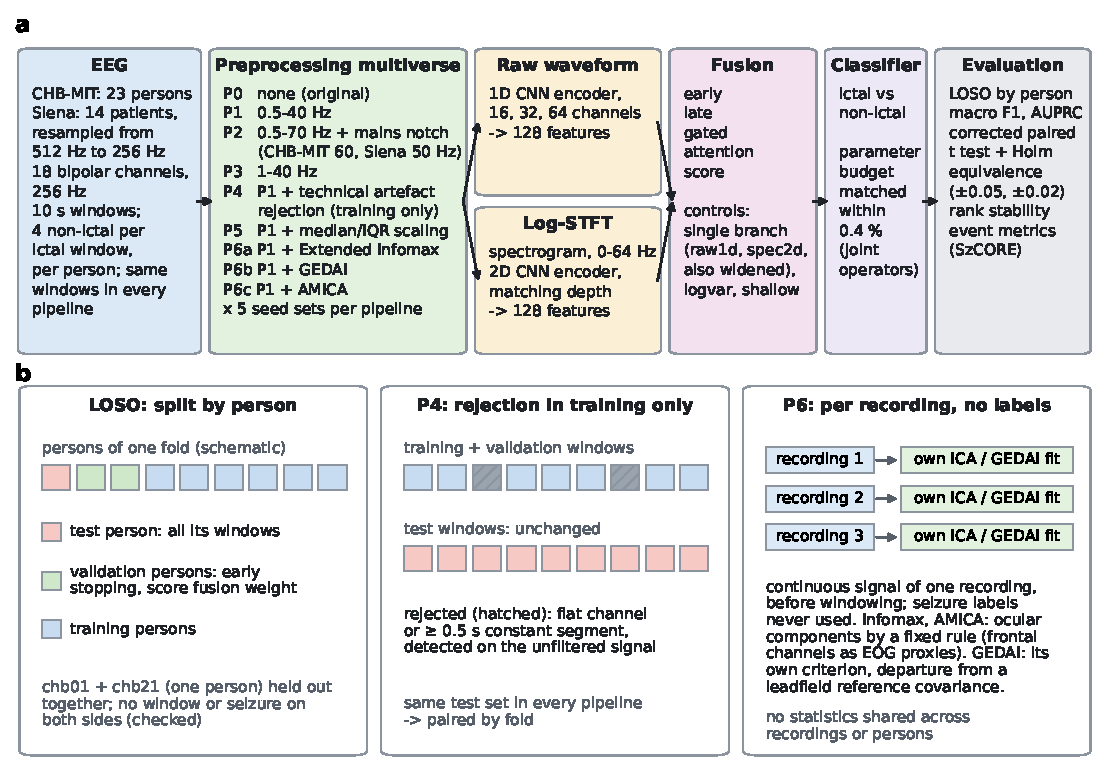
\includegraphics[width=1\linewidth,height=\textheight,keepaspectratio,alt={Study design. a, The multiverse: two datasets harmonised to 18 bipolar channels at 256 Hz and 10 s windows; nine preprocessing pipelines, each trained with five seed sets; a 1D CNN on the raw waveform and a 2D CNN on the log-STFT, combined by five fusion operators, four jointly trained under a matched parameter budget and score fusion as a decision-level ensemble of the two branches at their own size, with single-branch and classical controls; evaluation by leave-one-subject-out (LOSO) at the window and the seizure level. b, Where each step is applied and how leakage is prevented: whole persons are held out (chb01 and chb21 together), and validation persons serve only early stopping and the score fusion weight; P4 rejects windows from training and validation data only, so every pipeline is tested on the same windows; P6 cleans each recording on its own, without seizure labels.}]{figure1_design.pdf}
\caption{Study design. \textbf{a}, The multiverse: two datasets harmonised to 18 bipolar channels at 256 Hz and 10 s windows; nine preprocessing pipelines, each trained with five seed sets; a 1D CNN on the raw waveform and a 2D CNN on the log-STFT, combined by five fusion operators, four jointly trained under a matched parameter budget and score fusion as a decision-level ensemble of the two branches at their own size, with single-branch and classical controls; evaluation by leave-one-subject-out (LOSO) at the window and the seizure level. \textbf{b}, Where each step is applied and how leakage is prevented: whole persons are held out (chb01 and chb21 together), and validation persons serve only early stopping and the score fusion weight; P4 rejects windows from training and validation data only, so every pipeline is tested on the same windows; P6 cleans each recording on its own, without seizure labels.}\label{fig:1}
\end{figure}

\subsection{2.1 Datasets and EEG harmonisation}\label{datasets-and-eeg-harmonisation}

\textbf{CHB-MIT} (\citealp{Shoeb_2009}; \citealp{Goldberger_2000}) holds 686 scalp recordings, 982.9 h,
from 24 paediatric cases at 256 Hz in a bipolar montage. Two cases, chb01 and chb21,
are documented as the same person and are treated as one subject, which gives 23
subjects. We use the standard 18-channel bipolar (double banana) montage and keep the
683 recordings that contain all 18 channels, with 185 of the 198 annotated seizures in
the windowed corpus; the three dropped recordings belong to part of subject chb12's
data recorded in a different montage. Seizure annotations were parsed by order rather
than by their printed number, which corrects a labelling error in \nolinkurl{chb09_08.edf}
(\texttt{src/chbmit.py:\ parse\_summary}).

\textbf{Siena Scalp EEG} (\citealp{Detti_2020}) holds 41 recordings, 141.0 h by the EDF
headers, from 14 adult patients, with 47 annotated seizures, recorded at 512 Hz in a
referential 10-20 montage (older electrode names T3 to T6 are mapped to T7, T8, P7,
P8). Six problems in the published seizure lists (a seizure ending after its
recording, two conflicting onset or end times, two start times that disagree with the
EDF headers, an onset given only clinically) were resolved before any analysis, each
as either a correction verified against the recording or a stated decision rule;
Supplementary Table S4 lists every decision, how it was checked, its remaining
uncertainty, and how much the alternative would change the windows (\nolinkurl{docs/SIENA.md}).

\textbf{Harmonisation.} Siena is converted to the CHB-MIT form before anything else: the
18 bipolar channels are formed as electrode differences of the referential signals,
and the continuous recording is resampled from 512 to 256 Hz with a polyphase filter
(\nolinkurl{scipy.signal.resample_poly}, factor 1/2; \texttt{src/siena.py:\ read\_bipolar}). Both
corpora then pass through identical code. Seizure times are converted to seconds from
each recording's first sample using the EDF header start time (modulo 24 h for
recordings past midnight).

\textbf{Windows and labels.} Recordings are cut into non-overlapping 10 s windows. A window
is ictal if it overlaps an annotated seizure at all. Non-ictal windows are subsampled
per subject to four per ictal window of that subject, with a fixed seed, and every
subject's true recording duration is kept for the event metrics (Section 2.5). This
gives 6,380 windows (1,276 ictal) for CHB-MIT and 1,640 windows (328 ictal) for Siena,
exactly four non-ictal windows per ictal window in every subject. The CHB-MIT windows
come from 670 of the 683 recordings; no window was drawn from the other 13, all of them
without seizures. The same windows are used by every pipeline, which is checked
whenever a pipeline's corpus is built, so all comparisons between pipelines are paired
window by window.

\textbf{Class prevalence.} The fixed ratio gives every pipeline, operator and subject the
same class distribution, so that window-level results are comparable across them.
Consequently, the window-level evaluation reflects this controlled sampling
distribution, with 20 percent ictal windows, rather than the natural prevalence of
seizures in continuous EEG, which is far lower (0.4 percent of all 10 s windows of the
CHB-MIT recordings, 0.6 percent in Siena's recordings, which are cut around seizures). Window-level metrics, and macro F1 at a fixed threshold in particular, should
therefore be interpreted within this experimental setting and not as the performance
expected on continuous recordings. The seizure-level evaluation (Section 2.5) runs on
the original, complete recording timelines and complements it.

\textbf{Differences between the datasets.} The two corpora differ in age (mostly children
against adults), seizure types, recording length per patient (Siena's
recordings are cut around seizures for a seizure prediction study), centre,
equipment and mains frequency (60 Hz in Boston, 50 Hz in Italy). Results are
compared between them as an independent replication and a transfer test (RQ3), not
interpreted as an age or population effect: because the datasets differ in several of
these respects at once, no difference between them can be attributed to any single
one.

\subsection{2.2 Preprocessing multiverse}\label{preprocessing-multiverse}

Following the multiverse approach (\citealp{Steegen_2016}), nine defensible
preprocessing pipelines are crossed with every model, operator and seed instead of
choosing one. Each pipeline changes one hypothesis-driven aspect; windows, labels,
spectrogram settings, models, training and evaluation are fixed (\nolinkurl{src/preprocess.py}).

\begingroup\small

{\def\LTcaptype{none} % do not increment counter
\begin{longtable}[]{@{}
  >{\raggedright\arraybackslash}p{(\linewidth - 10\tabcolsep) * \real{0.1307}}
  >{\raggedright\arraybackslash}p{(\linewidth - 10\tabcolsep) * \real{0.1407}}
  >{\raggedright\arraybackslash}p{(\linewidth - 10\tabcolsep) * \real{0.1608}}
  >{\raggedright\arraybackslash}p{(\linewidth - 10\tabcolsep) * \real{0.1859}}
  >{\raggedright\arraybackslash}p{(\linewidth - 10\tabcolsep) * \real{0.1910}}
  >{\raggedright\arraybackslash}p{(\linewidth - 10\tabcolsep) * \real{0.1910}}@{}}
\toprule\noalign{}
\begin{minipage}[b]{\linewidth}\raggedright
Pipeline
\end{minipage} & \begin{minipage}[b]{\linewidth}\raggedright
Band-pass
\end{minipage} & \begin{minipage}[b]{\linewidth}\raggedright
Notch
\end{minipage} & \begin{minipage}[b]{\linewidth}\raggedright
Artefact handling
\end{minipage} & \begin{minipage}[b]{\linewidth}\raggedright
Normalisation
\end{minipage} & \begin{minipage}[b]{\linewidth}\raggedright
Question
\end{minipage} \\
\midrule\noalign{}
\endhead
\bottomrule\noalign{}
\endlastfoot
P0 & none & none & none & z-score & original benchmark \\
P1 & 0.5 to 40 Hz & none & none & z-score & standard EEG band \\
P2 & 0.5 to 70 Hz & mains (CHB-MIT 60 Hz, Siena 50 Hz) & none & z-score & information above 40 Hz \\
P3 & 1 to 40 Hz & none & none & z-score & low frequency content and drift \\
P4 & 0.5 to 40 Hz & none & technical artefact rejection (training only) & z-score & artefact rejection \\
P5 & 0.5 to 40 Hz & none & none & median and IQR & normalisation \\
P6a & 0.5 to 40 Hz & none & Extended Infomax ICA & z-score & artefact removal \\
P6b & 0.5 to 40 Hz & none & GEDAI & z-score & artefact removal \\
P6c & 0.5 to 40 Hz & none & AMICA & z-score & artefact removal \\
\end{longtable}
}

\endgroup

\textbf{Order of operations.} Each continuous recording is band-pass filtered, notch
filtered (P2) and cleaned (P6), in that order; it is then cut into the fixed windows,
P4's rejection rule is applied, and each window is normalised. The spectrogram is
computed from the normalised window.

\textbf{Filters.} Zero-phase Butterworth filters (order 4, forward and backward) are
applied to each continuous recording before it is windowed, so that no filter
transient falls at a window edge. P2's notch removes each dataset's own mains
frequency and its first harmonic; with a fixed 60 Hz notch Siena's P2 windows kept a
50 Hz line 318 times stronger than the 40 to 48 Hz background, so P2 was defined per
dataset and its Siena runs were repeated.

\textbf{Normalisation.} Each channel of each window is standardised on its own: z-score
(P0 to P4, P6) or median and interquartile range (P5). No statistic is computed across
windows, recordings or persons, so normalisation cannot carry information from test to
training data.

\textbf{P4, technical artefact rejection.} Amplitude was measured before a criterion was
chosen: every amplitude threshold removes seizures selectively (500~\(\mu\)V rejects 72
percent of CHB-MIT's ictal and 48 percent of its non-ictal windows), because ictal
windows have larger amplitudes. P4 therefore rejects only technical artefacts: a flat
channel (standard deviation below 1~\(\mu\)V in the window) or a constant run of at least
0.5 s on any channel (a signal dropout), detected on the unfiltered signal. In CHB-MIT
this rejects 42 of 1,276 ictal (3.3 percent) and 39 of 5,104 non-ictal windows (0.8
percent); the difference reflects which recordings have dropouts, not physiology
(Supplementary Table S3). In Siena it rejects one window. Rejected windows are removed
from training and validation only; the test windows are those of every other
pipeline.

\textbf{P6, three artefact removal algorithms.} P6 applies Extended Infomax ICA (\citealp{Lee_1999}; MNE-Python, \citealp{Gramfort_2013}), GEDAI (\citealp{Ros_2025}) or AMICA (\citealp{Palmer_2008}; \nolinkurl{jamica}) to the same 0.5 to 40 Hz signal, recording by recording.
Infomax and AMICA share every setting and one component rejection rule: 16 components
(the 18-channel bipolar montage has rank 16, because it contains two closed electrode
loops per hemisphere), fitted on every 8th sample, with components removed when their
correlation with any of the four frontopolar channels, used as EOG proxies since
neither dataset has an EOG channel, has \(|z| > 3\) (MNE \nolinkurl{find_bads_eog}). Muscle
components are not removed, because the gamma band carries the strongest ictal signal
in CHB-MIT. GEDAI is not an ICA: it removes what departs from a leadfield-based
reference covariance, by its own criterion, so the shared rule cannot apply. Its
reference covariance C, defined for a referential layout, is mapped onto the bipolar
montage as \(D\,C\,D^{\top}\) (D the electrode difference matrix), and the channel mean is removed
before and restored after cleaning. GEDAI's threshold preset was fixed before any
classification run, on signal preservation alone: on six CHB-MIT subjects the default
removed more than half of the power of 39 percent of recordings, the conservative
preset of 17 percent; the conservative preset removed no more from ictal than from
non-ictal windows, whereas the default kept a lower median share of the ictal power
(0.78 against 1.00; Supplementary Table S2); P6b uses the conservative preset. The comparison among P6a,
P6b and P6c is therefore a comparison of whole cleaning procedures: for Infomax and
AMICA it isolates the decomposition algorithm, while GEDAI differs also in how it
decides what to remove. Signal retention and compute are in Supplementary Table S1, and the power removed by band
and class in Supplementary Table S5.

\textbf{No leakage through P6.} Each recording is decomposed and cleaned on its own, from
its own unlabelled signal; seizure annotations are never used, and no decomposition,
threshold or statistic is shared between recordings or persons. A test person's
recordings are therefore cleaned exactly as they would be without any training data.

\textbf{Offline processing.} Filtering and artefact cleaning are applied to complete
recordings before windows are extracted, so a window's cleaned signal depends on data
recorded after it. These experiments therefore evaluate the robustness of offline
preprocessing and do not represent a causal, real-time seizure detection pipeline, in
which only past signal is available.

\subsection{2.3 EEG representations and fusion strategies}\label{eeg-representations-and-fusion-strategies}

\textbf{Representations.} Each 10 s window enters the network twice: as the 18-channel
waveform (2,560 samples per channel) and as its log-magnitude short-time Fourier
transform, log(1 + \textbar STFT\textbar), computed per channel with a 1 s Hann window, 0.5 s hop and
256-point FFT and cropped at 64 Hz (65 frequency bins by 19 frames;
\nolinkurl{src/chbmit_prep.py}). The 64 Hz ceiling is kept in every pipeline, so input shapes and
parameter counts never change.

\textbf{Architecture.} A 1D convolutional encoder (channel widths 16, 32, 64) processes the
waveform and a 2D convolutional encoder of matching depth the spectrogram; each yields
a 128-dimensional pooled feature vector. Five interchangeable fusion operators combine
them:

\begin{itemize}
\tightlist
\item
  \textbf{Early:} the waveform passes a small strided 1D encoder, is broadcast along the
  spectrogram's time axis and concatenated to it as an extra channel before the 2D
  backbone (architecturally an intermediate fusion, since the two inputs share no
  tensor shape).
\item
  \textbf{Late:} the two feature vectors are concatenated and classified by a small MLP.
\item
  \textbf{Gated:} a learned scalar gate per branch reweights the concatenated features.
\item
  \textbf{Attention:} a learned attention module weights the branches from both feature
  vectors jointly.
\item
  \textbf{Score:} the two branches are trained as independent classifiers and their
  probabilities blended, p = w p\_waveform + (1 - w) p\_spectrogram, with the weight w
  chosen on the validation subjects only, by minimising their log loss over a 41-point
  grid from 0 to 1.
\end{itemize}

\textbf{Parameter matching.} Every jointly trained model (the four joint operators and two
widened single-branch controls) is sized to a common budget by solving the fusion
head's hidden width numerically (\nolinkurl{src/models.py}): with 18 input channels the models
have 102,236 to 103,712 parameters, the four joint operators within 0.36 percent of
each other. Score fusion, an ensemble of two independently sized classifiers, keeps
its natural size: it blends the probabilities of the two default-width single-branch
controls below (28,850 and 34,546 parameters, 63,396 together, about 62 percent of the
budget). Score fusion is retained as a complementary decision-level strategy: because
its architecture and training differ from those of the jointly trained models, it is
part of the broader practical comparison of operators but not of the strictly
parameter-matched architectural comparison, which concerns early, late, gated and
attention fusion (102,547; 102,768; 102,921 and 102,767 parameters).

\textbf{Controls.} The two single-branch networks at their default width (raw1d, spec2d)
and widened to the fusion budget (raw1d\_wide, spec2d\_wide), which asks whether fusion
beats a unimodal model of the same size; and two classical baselines without
representation learning, a logistic regression on log variance (logvar) and on seven
hand-crafted features (log variance, line length and relative power in five bands;
shallow), 19 and 127 parameters with the intercept. The networks see the same windows
and preprocessing as the operators. The logistic regressions (standardised features,
class-balanced weights, C = 1, no tuning) need no early stopping, so they are fitted
on all training subjects, including the four (Siena: three) that the networks set aside
for validation; this favours the classical baselines, if anything.

\subsection{2.4 Experimental protocol}\label{experimental-protocol}

\textbf{Leave one subject out.} All evaluation is subject-independent. Each subject is held
out once as the test set (23 folds on CHB-MIT, 14 on Siena), and all recordings of one
individual are assigned to the same partition (chb01 and chb21 are held out together).
Within each outer fold, validation subjects are selected exclusively from the remaining
training subjects, and the held-out subject is excluded from all training, early
stopping and model selection. The selection is deterministic and does not look at
any result: the remaining subjects are ordered by their number of ictal windows, and
round(0.2 n) of them (4 of 22 on CHB-MIT, 3 of 13 on Siena) are taken at evenly spaced
positions of that order, so the validation set spans the range of seizure burdens and
always contains ictal windows. It serves early stopping and the score fusion weight
only. No subject's windows and no seizure's windows ever appear in two of the
training, validation and test partitions; an automatic check of every fold confirms
this for both datasets and that every stored run held out the same subjects in the
same folds (\nolinkurl{src/audit_methods.py}), and the leakage checker was itself validated on a
deliberately leaky split (\nolinkurl{src/chbmit_corpus.py}).

\textbf{Training.} AdamW (\citealp{Loshchilov_2019}), learning rate 1e-3, weight decay
1e-4, batch size 32, class-weighted cross-entropy; early stopping on validation macro
F1 with patience 12 after a minimum of 20 epochs, at most 60 epochs. The minimum guards
against a model stopping in a trivial single-class solution, found in an early audit.
These settings, and the architectures, were fixed before the multiverse runs and not
tuned: there was no hyperparameter search or optimisation, the same values were used
for every model, pipeline and dataset, and the validation subjects served only early
stopping and the score fusion weight. The reported performance is therefore that of a
fixed, untuned configuration rather than the best each operator could reach.

\textbf{Seeds.} Every pipeline is run with five seed sets. A run's seed for each fold and
model is derived from the seed set, fold and model (\texttt{src/config.py:\ fold\_seed}), so it
does not depend on execution order. It sets the weight initialisation, the order of
the mini-batches and the dropout masks. It does not change the data: the window
sampling (one fixed seed), the validation subjects (deterministic) and the artefact
cleaning (a seed per recording) are the same in every seed set, so differences between
seed sets reflect stochastic training alone. The ranking of the operators was unstable across
three seed sets (Kendall's W below 0.5 in seven of nine CHB-MIT pipelines); after these
three-seed results, the extension to five seed sets was decided,
to estimate the seed variance more reliably. It was not a rule fixed beforehand.

\textbf{Cross-dataset experiment (RQ3).} Each model is trained once on all CHB-MIT subjects
(with the same inner validation rule) and tested on every Siena window and recording,
for every pipeline and seed set (\nolinkurl{src/cross_dataset.py}). The pipeline is applied to
each dataset as defined, including each dataset's own mains notch in P2. Siena is
used for testing only: the validation subjects are drawn from CHB-MIT, and no Siena
window enters training, early stopping, the score fusion weight or any other choice.
Results are reported per Siena patient. The experiment asks whether the relative
performance of the operators persists when the dataset changes. Because the datasets
differ in population, acquisition and recording protocol (Section 2.1), it measures
their combined distribution shift and does not isolate any single source of it.

\subsection{2.5 Evaluation metrics}\label{evaluation-metrics}

\textbf{Window level (primary).} Macro F1 and the area under the precision-recall curve
(AUPRC) are primary; balanced accuracy (the mean of sensitivity and specificity) is
reported alongside, with AUROC and the Brier score as secondary. A window is
predicted ictal when its ictal probability exceeds 0.5, for every model and control
alike. AUPRC is computed as average precision (scikit-learn) from the predicted ictal
probability, with the ictal class as the positive class; it assesses how well the
probabilities rank ictal above non-ictal windows across all thresholds, complementing
the threshold-dependent macro F1. Metrics are computed per fold on the held-out
subject's windows and averaged over folds within a run, each fold with equal weight.
The subject is the unit of generalisation and of the statistical tests; pooling
windows instead would let the subjects with the most seizures dominate the average.

Window-level classification and seizure-level detection are evaluated separately
because they address different aspects of performance: macro F1 and AUPRC describe
classification under the controlled window sampling (Section 2.1), whereas
seizure-level sensitivity and false alarms per hour are assessed on the original
recording timelines with event-scoring rules fixed in advance. A model can classify
windows well and still miss seizures or raise many false alarms.

\textbf{Seizure level (secondary, clinical).} Every model saved for a fold is applied to
every 10 s window of every recording of the held-out subject, not only the subsampled
test windows, after the pipeline's own preprocessing; a window is positive when its
probability exceeds 0.5, with no further post-processing. Detections are scored
against the annotated seizures with SzCORE's event scoring (\citealp{Dan_2024};
\nolinkurl{timescoring} 0.0.7, defaults: 30 s tolerance before onset and 60 s after offset, any
overlap counts, events closer than 90 s merged, events longer than 5 min split).
Seizure-level sensitivity is the share of seizures detected; the false alarm rate is
false-positive events per hour on the true recording time. The scored recordings hold
187 seizures in 979.9 h (CHB-MIT) and 47 seizures in 141.0 h (Siena). On CHB-MIT these
are the 185 annotated seizures of the 683 recordings in the target montage (of 198 in
the dataset, Section 2.1); one of them, in chb11\_99, lasts 752 s and is split by the
5 min rule into three reference events, and in no other recording does merging or
splitting change the count (\nolinkurl{results_v2/audit/methods_audit.md}). Scoring the
window labels themselves as predictions detects all of them without a false alarm,
which checks the reference, the windows and the scoring together. On Siena only
sensitivity is reported: its recordings are cut around seizures, so a false alarm
rate would not describe continuous monitoring. The criterion, the merging of
consecutive detections and the counting of false alarms were fixed, and committed,
before any multiverse run (\nolinkurl{docs/EVENTS.md}), and are the same for every operator and
pipeline.

\subsection{2.6 Statistical analysis}\label{statistical-analysis}

\textbf{Pairwise comparisons.} Leave-one-subject-out folds share training data, so the
standard paired test overstates significance; in a simulation of two equivalent
classifiers the naive paired Wilcoxon test rejected in 37.6 percent of cases at a
nominal 5 percent (\nolinkurl{src/sim_cv_correlation.py}). On the Bonn corpus, studied in an
earlier stage of this project, the naive test found 13 to 22 significant pairs among
55 per task and the corrected test none among the deep models (Supplementary Note 1).
Because LOSO training sets overlap substantially, pairs of operators are compared with
the resampling-corrected paired t test (\citealp{Nadeau_2003}) rather than treating
the held-out folds as independent observations. The test inflates the variance of the
mean fold difference from var(d)/k to (1/k + n\_test/n\_train) var(d), on k - 1 degrees
of freedom. We count subjects: n\_test/n\_train = 1/22 on CHB-MIT and 1/13 on Siena, the
held-out subject against the subjects outside it. Since 4 (Siena: 3) of these serve as
validation subjects, the networks are fitted on 18 (10); with that conservative ratio,
1/18 and 1/10, no operator pair becomes significant and the pairs equivalent within
0.05 fall from 73 to 70 of 90 on CHB-MIT and from 21 to 19 on Siena
(\nolinkurl{results_v2/audit/methods_audit.md}). Subjects contribute different numbers of
windows, but each fold enters the test as one observation (Section 2.5). Seed sets are
averaged within each fold before testing, so the five seed sets and nine pipelines
never inflate the number of independent observations, which is always the number of
subjects.

Multiplicity is addressed with Holm correction within predefined families: the ten
operator pairs of one pipeline, for one dataset and metric, form one family (nine
families per dataset); the 30 comparisons of the six controls with the five operators
in one pipeline form another.

\textbf{Practical equivalence.} For each pair the two one-sided test with the same
corrected variance gives the smallest margin within which the pair is equivalent at
alpha = 0.05; a pair is equivalent if that margin is at most 0.05 macro F1 (main
analysis) and, as a stricter sensitivity analysis, 0.02. Both margins were fixed and
committed before any multiverse result existed. A pair is robustly equivalent if it is
equivalent in every pipeline. Statistical significance and practical equivalence are
assessed separately: failure to reject equal performance is not interpreted as
evidence of equivalence. The corrected test, the equivalence bound, the Holm
adjustment and Kendall's W were checked against independent re-implementations
(\nolinkurl{src/audit_methods.py}).

\textbf{Ranking stability.} In every run (pipeline and seed set) the five operators are
ranked by mean macro F1. We report each operator's full rank distribution (counts per
rank, median, best and worst rank, share of runs won and lost), Kendall's W across
seed sets within each pipeline, and Kendall's tau between the seed-averaged rankings of
every pair of pipelines. Whether preprocessing changes the ranking more than the seed
does is tested by comparing the mean tau between seed sets of the same pipeline with
the mean tau between pipelines, against a null distribution from 10,000 permutations
of the pipeline labels within each seed set; the same test is run among P6a, P6b and
P6c alone.

\textbf{Fusion x Preprocessing.} A repeated-measures ANOVA on macro F1 (seed means) treats
the held-out subjects as the repeated units and pipeline and operator as within-subject
factors; each effect is tested against its interaction with subject, with
Greenhouse-Geisser correction. Effect sizes are reported as partial eta squared.

\textbf{Variance components.} For macro F1, AUPRC and balanced accuracy, the fully crossed
subject x pipeline x operator x seed design is decomposed as y = mu + subject +
pipeline + operator + seed + every interaction, all treated as random effects
(generalizability theory) and estimated by the method of moments from the expected
mean squares. With one observation per cell the four-way interaction is the residual.
Every component is reported unrounded, as an estimated variance, as a standard
deviation in the metric's own units (a practical size) and as a share of the total;
negative estimates, which arise when an effect's mean square is smaller than its error
term, are reported as such and set to zero in the shares. The components are
descriptive estimates of the variability associated with the held-out subject, the
pipeline, the operator and stochastic training. A share of zero is therefore not proof
that an effect is absent, and the subject component is read as subject-associated
variability: it collects everything that differs between held-out subjects, of which
individual physiology is only one part, together with seizure count and type, recording
length and recording conditions.

\textbf{Prediction stability.} The agreement (Cohen's kappa) of window-level predictions
between pipelines at the same seed set is compared with the agreement between seed
sets in the same pipeline.

Statistical significance is reported from the corrected tests and the ANOVA, practical
size from the equivalence margins and the variance components in metric units, and
ranking stability from the rank analyses; a result in one of these three is never
used as evidence for another. All analyses are implemented in \nolinkurl{src/multiverse.py} and
were validated on synthetic runs with known effects (39 checks).

\subsection{2.7 Reproducibility and computational cost}\label{reproducibility-and-computational-cost}

\textbf{Software and hardware.} Two environments were used (Table 2); artefact removal
needs a newer numpy than the training code and runs in its own environment
(\nolinkurl{requirements.txt}, \nolinkurl{requirements-ica.txt}). The software versions and the hardware of
every run are recorded in its \nolinkurl{meta.json}.

\begingroup\small

\begin{longtable}[]{@{}
  >{\raggedright\arraybackslash}p{(\linewidth - 4\tabcolsep) * \real{0.1759}}
  >{\raggedright\arraybackslash}p{(\linewidth - 4\tabcolsep) * \real{0.3668}}
  >{\raggedright\arraybackslash}p{(\linewidth - 4\tabcolsep) * \real{0.4573}}@{}}
\caption{Computational environments.}\tabularnewline
\toprule\noalign{}
\begin{minipage}[b]{\linewidth}\raggedright
\end{minipage} & \begin{minipage}[b]{\linewidth}\raggedright
Training and window-level evaluation
\end{minipage} & \begin{minipage}[b]{\linewidth}\raggedright
Artefact removal (P6) and seizure-level evaluation
\end{minipage} \\
\midrule\noalign{}
\endfirsthead
\toprule\noalign{}
\begin{minipage}[b]{\linewidth}\raggedright
\end{minipage} & \begin{minipage}[b]{\linewidth}\raggedright
Training and window-level evaluation
\end{minipage} & \begin{minipage}[b]{\linewidth}\raggedright
Artefact removal (P6) and seizure-level evaluation
\end{minipage} \\
\midrule\noalign{}
\endhead
\bottomrule\noalign{}
\endlastfoot
Used for & all LOSO and cross-dataset runs (135 runs) & the P6 corpora; applying the saved models to every window of every recording \\
Machine & lab PC: 2 x Intel Xeon (Skylake-SP), 64 logical CPUs; NVIDIA GeForce RTX 5070 & laptop: Intel Core Ultra 7 155U, 14 logical CPUs; no CUDA GPU \\
Operating system & Windows 10 (build 19045) & Windows 11 (build 26300) \\
Python & 3.12.10 & 3.12.7 \\
Numerical libraries & PyTorch 2.8.0 (CUDA 12.8 build), numpy 1.26.4, scipy 1.16.1, scikit-learn 1.7.2 & PyTorch 2.8.0 (CPU build), numpy 2.5.3 (OpenBLAS), scipy 1.16.1, scikit-learn 1.7.2, MNE 1.13.2, GEDAI 0.60, jamica 0.3.0, timescoring 0.0.7 \\
Threads & 16 CPU threads & 14 (BLAS) \\
Seeds & per seed set, fold and model (\nolinkurl{fold_seed}) & per recording, from its file name (crc32) \\
Determinism & PyTorch deterministic algorithms on the GPU & CPU only \\
\end{longtable}

\endgroup

\textbf{Determinism and device.} All training runs of one analysis use one machine, one device and
16 CPU threads, and CPU and GPU runs are never mixed in one analysis. On the CPU a run
was reproduced bit for bit, also with two runs sharing the machine. The multiverse ran
on the GPU with PyTorch's deterministic algorithms; adaptive average pooling has no
deterministic CUDA backward, yet two GPU runs of the same fold were identical. Before
switching to the GPU, its agreement with the CPU was tested at identical seeds: over
five folds the mean absolute macro F1 difference between CPU and GPU was 0.074,
slightly larger than the 0.066 between two CPU seed sets (\texttt{python\ -m\ src.compare\_runs};
\nolinkurl{docs/PIPELINE.md}). The criterion fixed beforehand, a CPU-GPU difference no larger than
the difference between seed sets, was therefore narrowly missed. The CPU-GPU difference
is comparable in size to the variation between stochastic training runs; this similarity
does not establish that hardware-related numerical differences and seed effects arise
from the same mechanism, and we make no claim about the cause.

\textbf{Reproducibility conditions.} Reproducibility was examined at the level of the
preprocessing and of the downstream predictions (Table 3). Identical preprocessing
configurations were run in different computational environments, and the differences
in the cleaned signals were followed into the classification and seizure-level
metrics.

\begingroup\small

\begin{longtable}[]{@{}
  >{\raggedright\arraybackslash}p{(\linewidth - 6\tabcolsep) * \real{0.2000}}
  >{\raggedright\arraybackslash}p{(\linewidth - 6\tabcolsep) * \real{0.2650}}
  >{\raggedright\arraybackslash}p{(\linewidth - 6\tabcolsep) * \real{0.2600}}
  >{\raggedright\arraybackslash}p{(\linewidth - 6\tabcolsep) * \real{0.2750}}@{}}
\caption{What was held fixed and what varied in each reproducibility comparison.}\tabularnewline
\toprule\noalign{}
\begin{minipage}[b]{\linewidth}\raggedright
Comparison
\end{minipage} & \begin{minipage}[b]{\linewidth}\raggedright
Held fixed
\end{minipage} & \begin{minipage}[b]{\linewidth}\raggedright
Varied
\end{minipage} & \begin{minipage}[b]{\linewidth}\raggedright
Measured
\end{minipage} \\
\midrule\noalign{}
\endfirsthead
\toprule\noalign{}
\begin{minipage}[b]{\linewidth}\raggedright
Comparison
\end{minipage} & \begin{minipage}[b]{\linewidth}\raggedright
Held fixed
\end{minipage} & \begin{minipage}[b]{\linewidth}\raggedright
Varied
\end{minipage} & \begin{minipage}[b]{\linewidth}\raggedright
Measured
\end{minipage} \\
\midrule\noalign{}
\endhead
\bottomrule\noalign{}
\endlastfoot
Training, repeat on CPU & code, data, seeds, machine, threads & nothing (also two runs sharing the machine) & fold metrics: bit-identical \\
Training, repeat on GPU & code, data, seeds, machine, GPU, deterministic mode & nothing & fold metrics: identical \\
Training, CPU against GPU & code, data, seeds, machine & device (CPU or GPU) & macro F1 difference, against that between seed sets \\
Artefact removal, two machines & code, input recordings, package versions, seeds, BLAS kernel & machine (laptop, lab PC), thread count & components removed, power kept, per recording; 670 CHB-MIT recordings \\
Artefact removal, same machine & code, input, versions, seeds, machine & process parallelism (run alone or in parallel workers) & as above \\
Artefact removal, third machine & code, input, versions, seeds & architecture (ARM, macOS) & as above, on a subset of recordings \\
Rounding perturbation & everything & input multiplied by 1 + 1e-7 N(0, 1) & as above \\
Effect on outcomes & trained models, test recordings & cleaned signals (training-time against event-time cleaning) & seizure-level sensitivity, false alarms, rankings \\
\end{longtable}

\endgroup

\textbf{Reproducibility of artefact removal.} Fixing seeds and package versions did not
make P6 reproducible across machines and execution contexts (\nolinkurl{docs/ICA_REPRO.md}).
AMICA removed the same components in every recording on every machine and in every
execution context; the power it kept differed by at most 0.003 between machines and
0.0007 between two runs on the same machine. Extended Infomax removed different components in
recordings whose component lay near the \textbar z\textbar{} = 3 rule: 2.5 percent of recordings between
two machines and 1.2 percent between two runs on the same machine with different
process parallelism. GEDAI was deterministic on each machine but gave a different
result on the second machine in 27 percent of recordings, often by a large amount.
A third machine of another architecture (ARM) agreed with the other two on recordings
where they agreed, and often with neither where they differed. Multiplying the input by
(1 + 1e-7 N(0, 1)), a rounding-level perturbation, changed GEDAI's result on exactly the
recordings that differed between machines, also on a full-rank montage, and Infomax's
component decision on recordings where it had differed; AMICA was unchanged. This is
consistent with a sensitivity of the methods to rounding near a decision threshold on
particular recordings rather than with a fault of one machine or library, but it does
not identify the numerical mechanism, and the differences are reported as an empirical
reproducibility limitation. All three methods were compared on the same criteria: the
components removed and the share of signal power kept, per recording.
Window-level results are unaffected, because every P6 training and test window comes
from one set of signals, cleaned once. The event metrics, which need every recording
cleaned again, were computed on the machine that produced those signals; they then
reproduce the training-time cleaning exactly for GEDAI, within 1.4 percent of the
amplitude for AMICA, and differ for Infomax in 8 of 670 CHB-MIT recordings
(\nolinkurl{events/meta.json}, \nolinkurl{window_check}).

\textbf{Computational cost.} Artefact removal of the 670 CHB-MIT recordings with selected
windows took 4.7 (GEDAI), 8.5 (Infomax) and 73 (AMICA) CPU hours on a laptop CPU
(Supplementary Table S1). One CHB-MIT run (23 folds, nine models) took about 1.5 h on
the GPU, one Siena run about a quarter of an hour, and one cross-dataset run about
5 min; training one fold (all nine models) took 3.5 to 6 min on the GPU against 16 to
17 min on the CPU (\nolinkurl{perfold.csv}).

\textbf{Availability.} Code, the per-fold results of every run, and all analyses are in the
public repository, whose README lists the commands that regenerate each table and figure.
Following our own recommendation (Section 4.5), the repository also holds, per recording
and artefact removal method, the outcome of the cleaning the models were trained and
tested on (components removed, GEDAI's threshold, power kept;
\nolinkurl{results_v2/qc/p6_recording_logs.csv}) and of the recleaning used for the event metrics
(\nolinkurl{p6_recording_logs_events.csv}), so that a reader can check a reproduction recording
by recording.

\section{3. Results}\label{results}

The evaluation comprised nine preprocessing pipelines, five seed sets and five fusion
operators, together with single-branch neural-network and classical controls. Each
pipeline-seed configuration was evaluated with leave-one-subject-out (LOSO)
cross-validation on CHB-MIT (23 subjects) and Siena (14 subjects), giving 45 runs per
dataset; 45 further runs evaluated transfer from CHB-MIT to Siena
(\nolinkurl{results_v2/multiverse/chbmit_cuda}, \nolinkurl{results_v2/multiverse/siena_cuda},
\nolinkurl{results_v2/cross}). Means over runs are given with the standard deviation over runs.

The results are presented in seven stages. We first examine whether fusion operators
offer a meaningful performance advantage and whether it justifies their architectural
complexity. We then distinguish statistical significance from practical equivalence,
assess the stability of the operators' ranking across pipelines and seeds, and identify
the principal sources of performance variability. Finally, we examine the effects and
the reproducibility of artefact removal, the seizure-level detection, and whether the
performance patterns generalise across datasets.

\subsection{3.1 Fusion complexity does not consistently translate into superior performance}\label{fusion-complexity-does-not-consistently-translate-into-superior-performance}

The five fusion operators reached broadly comparable window-level performance across
the preprocessing multiverse, although their relative behaviour differed between
datasets (Table 4, Figure 2).

On CHB-MIT, mean macro F1 over the 45 runs ranged from 0.673 \(\pm 0.017\) for score fusion to
0.686 \(\pm 0.016\) for gated fusion; early, late and attention fusion reached 0.677 \(\pm 0.013\),
0.681 \(\pm 0.015\) and 0.683 \(\pm 0.014.\) Within a pipeline, the best and the worst operator
differed by 0.013 to 0.035 macro F1 (median 0.021), and each operator's mean varied
little across pipelines (SD 0.007 to 0.008).

On Siena, the operators differed more. Score fusion reached the highest mean macro F1
(0.670 \(\pm 0.024\)), followed by late (0.640 \(\pm 0.025\)), gated (0.631 \(\pm 0.031\)), attention
(0.625 \(\pm 0.023\)) and early fusion (0.617 \(\pm 0.021\)). Within a pipeline the best and the worst
operator differed by 0.042 to 0.070 (median 0.053), and the variation across pipelines
was larger than on CHB-MIT (SD 0.011 to 0.024). The separation between operators was
therefore dataset-dependent, and its size has to be weighed against its uncertainty
(Section 3.2) rather than read as superiority from mean performance alone.

Increasing architectural complexity did not consistently improve performance. The
spectrogram network widened to the fusion budget reached a mean macro F1 of 0.683 on
CHB-MIT, within the range of the jointly trained operators (0.677 to 0.686), and 0.663
on Siena, above every jointly trained operator (0.617 to 0.640) and below only score
fusion (0.670); it exceeded the best operator of a run in 9 (CHB-MIT) and 16 (Siena) of
45 runs. The waveform network was weaker (0.662 and 0.612 at the fusion budget, 0.663 and
0.609 at default width), and widening either branch to the fusion budget changed little
(Supplementary Table S7). The shallow classifier, a logistic regression with 127
parameters on seven hand-crafted features per channel, was equally competitive: its
mean macro F1 was 0.690 on CHB-MIT, above the best operator of a run in 12 of 45 runs,
and 0.720 on Siena, above the best operator in 43 of 45 runs and in all nine pipelines.
This advantage depends on the decision threshold on CHB-MIT, where the shallow
classifier's macro F1 is the lowest of all models at 0.3 (0.642) and the highest at 0.7
(0.715), but not on Siena, where it is the highest at 0.3, 0.5 and 0.7
(\nolinkurl{results_v2/sensitivity_preds/summary.md}).

These descriptive advantages did not amount to statistically significant superiority.
Tested like the operator pairs (corrected test, Holm across the 30 control-operator
comparisons of a pipeline; \nolinkurl{src/controls_stats.py}), no control differed significantly
from any operator in any pipeline of either dataset, in macro F1 or AUPRC; the smallest
corrected p was 0.12 (shallow against early fusion on Siena), and equivalence within
0.05 macro F1 could be shown in 34 of 270 comparisons on CHB-MIT and 13 of 270 on Siena
(Figure 2c, f). The controls therefore stood to the operators as the operators stood to
each other, and the additional complexity of multimodal fusion was not accompanied by a
reliable improvement in macro F1 under the conditions evaluated.

Classification at a threshold and the ranking of windows by probability behaved
differently. On CHB-MIT gated fusion had the highest mean AUPRC (0.666 \(\pm 0.018\)) and early
fusion the lowest (0.613 \(\pm 0.024\)); on Siena early fusion reached 0.496 \(\pm 0.035\) against
0.631 \(\pm 0.033\) for score fusion. Early fusion had the lowest AUPRC in all nine pipelines
of both datasets (0.564 to 0.632 on CHB-MIT against at least 0.631 for every other
operator, 0.453 to 0.540 on Siena against at least 0.522), although its macro F1 at the
0.5 threshold differed much less. On CHB-MIT the fused models ranked windows better on
average than a single branch (late, gated, attention and score fusion 0.655 to 0.666
against at most 0.618); on Siena the difference from the best single branch (0.581) was
inconsistent, from -0.085 (early fusion) to +0.050 (score fusion). Score fusion, which
blends the two default-width single-branch networks, had the lowest Brier score of all
models (0.265 and 0.304), and early fusion the highest among the operators on CHB-MIT
(0.330 against 0.294 to 0.300). Fusion complexity, thresholded classification and
probability ranking are therefore distinct properties: an operator can reach a
competitive macro F1 without discriminating equally well across thresholds.

\begingroup\small

\begin{longtable}[]{@{}
  >{\raggedright\arraybackslash}p{(\linewidth - 12\tabcolsep) * \real{0.1700}}
  >{\raggedright\arraybackslash}p{(\linewidth - 12\tabcolsep) * \real{0.1400}}
  >{\raggedright\arraybackslash}p{(\linewidth - 12\tabcolsep) * \real{0.1350}}
  >{\raggedright\arraybackslash}p{(\linewidth - 12\tabcolsep) * \real{0.1450}}
  >{\raggedright\arraybackslash}p{(\linewidth - 12\tabcolsep) * \real{0.1350}}
  >{\raggedright\arraybackslash}p{(\linewidth - 12\tabcolsep) * \real{0.1350}}
  >{\raggedright\arraybackslash}p{(\linewidth - 12\tabcolsep) * \real{0.1400}}@{}}
\caption{\textbf{Window-level performance of the fusion operators and the main controls}, mean and SD over the 45 runs of each dataset (fold means within a run). Per pipeline: Figure 2 and Supplementary Table S6; all six controls with their parameter counts: Supplementary Table S7.}\tabularnewline
\toprule\noalign{}
\begin{minipage}[b]{\linewidth}\raggedright
Model
\end{minipage} & \begin{minipage}[b]{\linewidth}\raggedright
CHB-MIT macro F1
\end{minipage} & \begin{minipage}[b]{\linewidth}\raggedright
CHB-MIT AUPRC
\end{minipage} & \begin{minipage}[b]{\linewidth}\raggedright
CHB-MIT bal. acc.
\end{minipage} & \begin{minipage}[b]{\linewidth}\raggedright
Siena macro F1
\end{minipage} & \begin{minipage}[b]{\linewidth}\raggedright
Siena AUPRC
\end{minipage} & \begin{minipage}[b]{\linewidth}\raggedright
Siena bal. acc.
\end{minipage} \\
\midrule\noalign{}
\endfirsthead
\toprule\noalign{}
\begin{minipage}[b]{\linewidth}\raggedright
Model
\end{minipage} & \begin{minipage}[b]{\linewidth}\raggedright
CHB-MIT macro F1
\end{minipage} & \begin{minipage}[b]{\linewidth}\raggedright
CHB-MIT AUPRC
\end{minipage} & \begin{minipage}[b]{\linewidth}\raggedright
CHB-MIT bal. acc.
\end{minipage} & \begin{minipage}[b]{\linewidth}\raggedright
Siena macro F1
\end{minipage} & \begin{minipage}[b]{\linewidth}\raggedright
Siena AUPRC
\end{minipage} & \begin{minipage}[b]{\linewidth}\raggedright
Siena bal. acc.
\end{minipage} \\
\midrule\noalign{}
\endhead
\bottomrule\noalign{}
\endlastfoot
early & 0.677~\(\pm 0.013\) & 0.613~\(\pm 0.024\) & 0.682~\(\pm 0.011\) & 0.617~\(\pm 0.021\) & 0.496~\(\pm 0.035\) & 0.642~\(\pm 0.022\) \\
late & 0.681~\(\pm 0.015\) & 0.656~\(\pm 0.019\) & 0.679~\(\pm 0.012\) & 0.640~\(\pm 0.025\) & 0.599~\(\pm 0.040\) & 0.679~\(\pm 0.018\) \\
gated & 0.686~\(\pm 0.016\) & 0.666~\(\pm 0.018\) & 0.683~\(\pm 0.013\) & 0.631~\(\pm 0.031\) & 0.591~\(\pm 0.034\) & 0.674~\(\pm 0.022\) \\
attention & 0.683~\(\pm 0.014\) & 0.655~\(\pm 0.020\) & 0.682~\(\pm 0.013\) & 0.625~\(\pm 0.023\) & 0.580~\(\pm 0.034\) & 0.667~\(\pm 0.020\) \\
score & 0.673~\(\pm 0.017\) & 0.655~\(\pm 0.017\) & 0.678~\(\pm 0.015\) & 0.670~\(\pm 0.024\) & 0.631~\(\pm 0.033\) & 0.689~\(\pm 0.022\) \\
raw1d\_wide (control) & 0.662~\(\pm 0.012\) & 0.605~\(\pm 0.017\) & 0.673~\(\pm 0.010\) & 0.612~\(\pm 0.028\) & 0.577~\(\pm 0.033\) & 0.657~\(\pm 0.019\) \\
spec2d\_wide (control) & 0.683~\(\pm 0.014\) & 0.618~\(\pm 0.016\) & 0.680~\(\pm 0.013\) & 0.663~\(\pm 0.026\) & 0.581~\(\pm 0.027\) & 0.681~\(\pm 0.021\) \\
shallow (control) & 0.690~\(\pm 0.008\) & 0.640~\(\pm 0.008\) & 0.739~\(\pm 0.007\) & 0.720~\(\pm 0.019\) & 0.667~\(\pm 0.015\) & 0.770~\(\pm 0.017\) \\
\end{longtable}

\endgroup

\begin{figure}
\centering
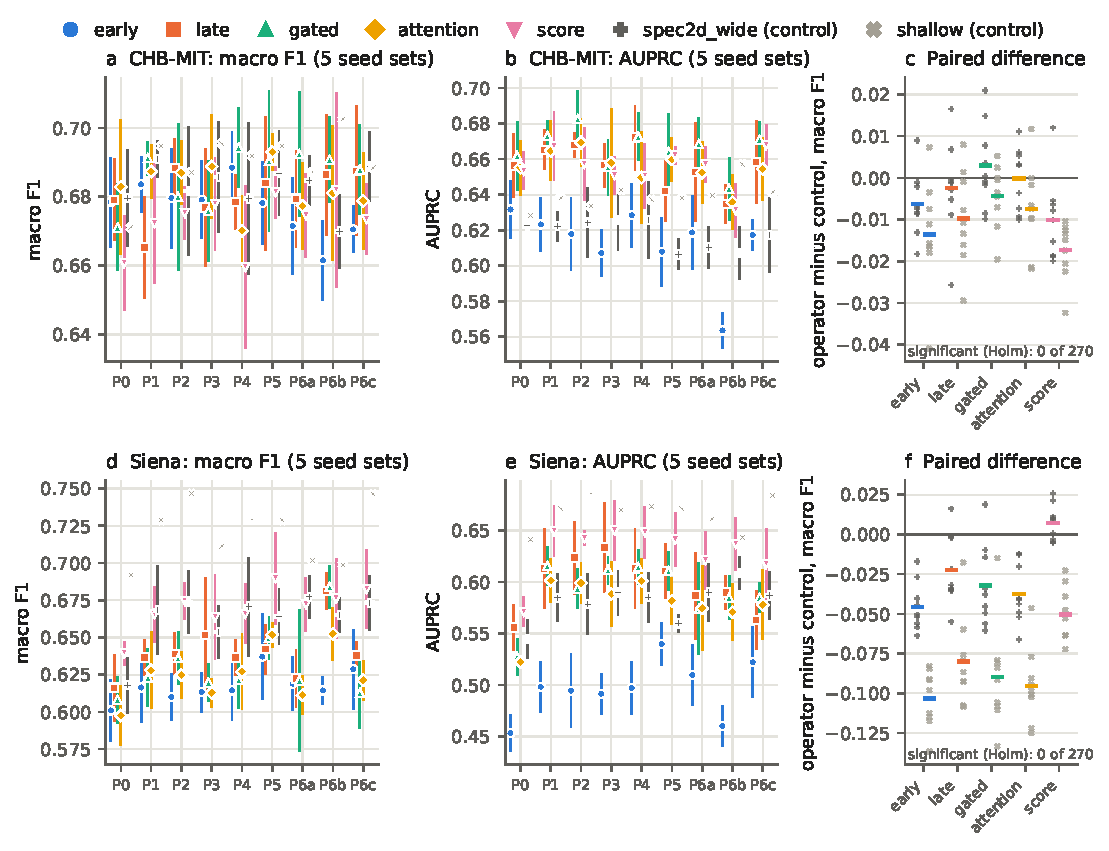
\includegraphics[width=1\linewidth,height=\textheight,keepaspectratio,alt={Fusion operators against the controls. a, b, d, e, Macro F1 and AUPRC of each operator and of two controls (the spectrogram network of the fusion budget, spec2d\_wide, and the shallow logistic regression) in each preprocessing pipeline, on CHB-MIT (a, b; 23 LOSO folds) and Siena (d, e; 14 folds); mean and SD over five seed sets, each run averaged over its folds. c, f, Paired difference in macro F1 between each operator and each control, one point per pipeline (fold values averaged over seed sets), with the mean as a bar; none of the 270 control-operator comparisons per dataset was significant after Holm correction.}]{figure2_performance.pdf}
\caption{Fusion operators against the controls. \textbf{a, b, d, e}, Macro F1 and AUPRC of each operator and of two controls (the spectrogram network of the fusion budget, spec2d\_wide, and the shallow logistic regression) in each preprocessing pipeline, on CHB-MIT (a, b; 23 LOSO folds) and Siena (d, e; 14 folds); mean and SD over five seed sets, each run averaged over its folds. \textbf{c, f}, Paired difference in macro F1 between each operator and each control, one point per pipeline (fold values averaged over seed sets), with the mean as a bar; none of the 270 control-operator comparisons per dataset was significant after Holm correction.}\label{fig:2}
\end{figure}

\subsection{3.2 Small performance differences do not establish practical equivalence}\label{small-performance-differences-do-not-establish-practical-equivalence}

The narrow differences between operators called for a formal distinction between
statistical significance and practical equivalence (Figure 3).

In both datasets, none of the 90 pairwise operator comparisons (10 pairs in each of nine
pipelines) was significant after Holm correction; the smallest corrected p was 0.19 on
CHB-MIT and 0.095 on Siena. The absence of a significant difference, however, did not
mean that the operators were practically equivalent.

At the margin of \(\pm 0.05\) macro F1 fixed in advance, 73 of the 90 comparisons on CHB-MIT
were equivalent, and two pairs, late-attention and gated-attention, were equivalent in
all nine pipelines. At the stricter margin of \(\pm 0.02\) only one comparison was. On Siena the
evidence for equivalence was much weaker: 21 of 90 comparisons were equivalent within
\(\pm 0.05\), no pair in every pipeline, and none within \(\pm 0.02.\) The smallest margin at which
equivalence could be shown had a median of 0.040 on CHB-MIT (0.020 to 0.066) and 0.081
on Siena (0.021 to 0.148).

The two datasets therefore supported different inferences. CHB-MIT showed that many
operators differ by less than a moderate margin, whereas Siena often lacked the precision
to establish either a difference or equivalence. The results thus fall into three kinds:
statistically detectable differences (none here), demonstrated practical equivalence,
and inconclusive comparisons; treating every non-significant result as equivalence would
have hidden this distinction. Supplementary Table S8 gives every paired difference with
its confidence interval, corrected p and equivalence margin.

\begin{figure}
\centering
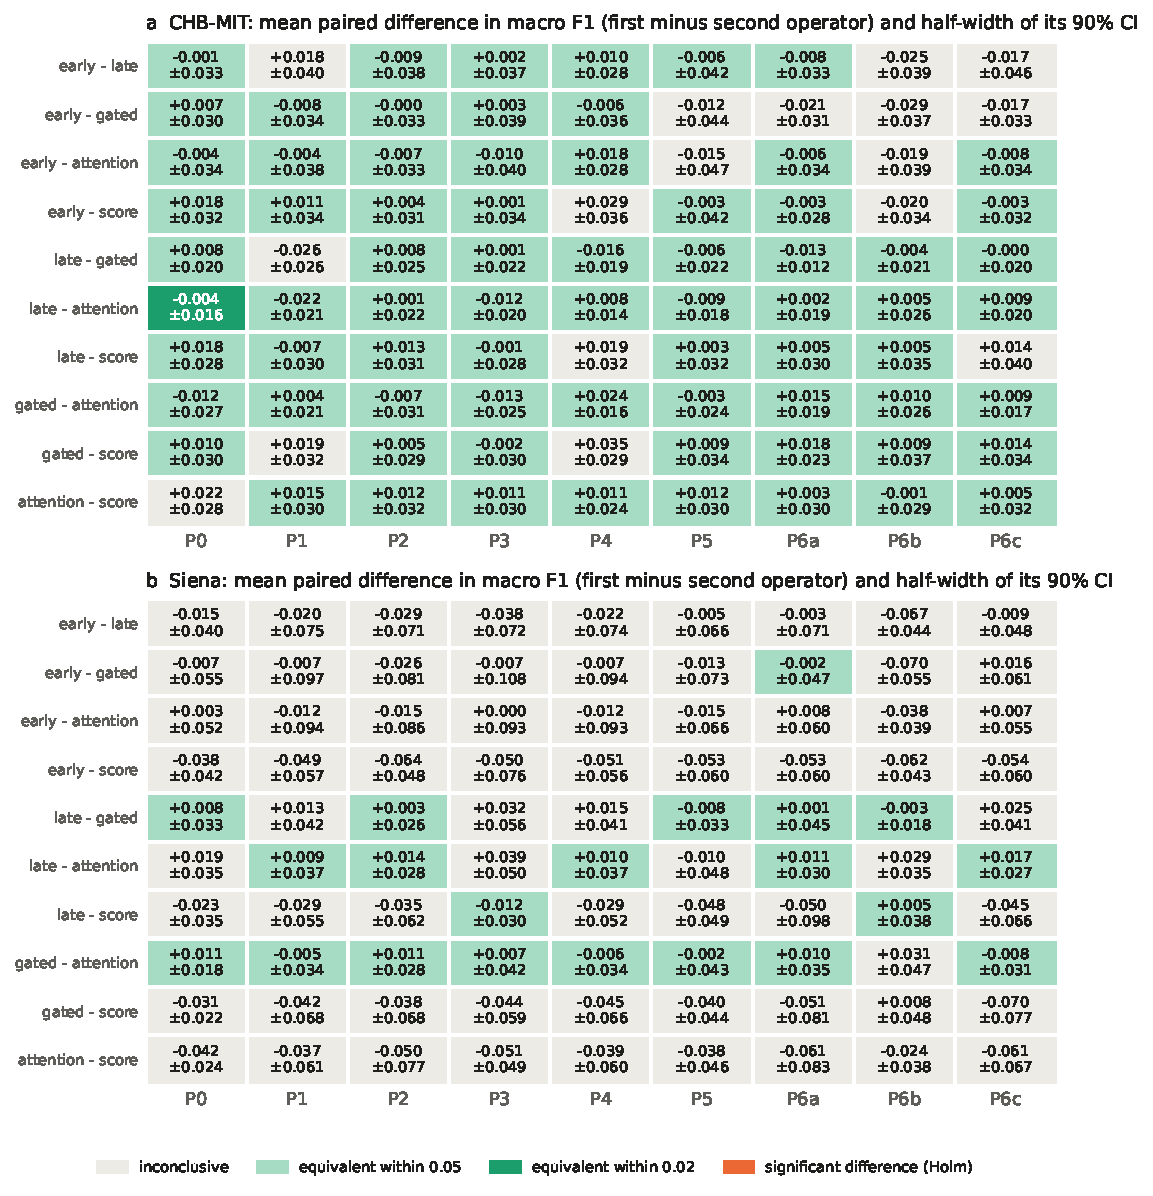
\includegraphics[width=1\linewidth,height=\textheight,keepaspectratio,alt={Equivalence matrix. For every operator pair (rows) in every preprocessing pipeline (columns): the mean paired difference in macro F1 (first minus second operator, fold values averaged over five seed sets) and the half-width of its 90 percent confidence interval with the corrected variance; the colour gives the outcome of the two one-sided tests at the margins of \textbackslash pm 0.05 and \textbackslash pm 0.02 and of the Holm-corrected test of a difference. a, CHB-MIT. b, Siena.}]{figure3_equivalence.pdf}
\caption{Equivalence matrix. For every operator pair (rows) in every preprocessing pipeline (columns): the mean paired difference in macro F1 (first minus second operator, fold values averaged over five seed sets) and the half-width of its 90 percent confidence interval with the corrected variance; the colour gives the outcome of the two one-sided tests at the margins of \(\pm 0.05\) and \(\pm 0.02\) and of the Holm-corrected test of a difference. \textbf{a}, CHB-MIT. \textbf{b}, Siena.}\label{fig:3}
\end{figure}

\subsection{3.3 Operator rankings are sensitive to the seed and to preprocessing decisions}\label{operator-rankings-are-sensitive-to-the-seed-and-to-preprocessing-decisions}

Although the mean differences were modest, which operator ranked first varied
substantially between runs (Figure 4).

On CHB-MIT gated fusion ranked first in 38 percent of runs, followed by attention (24),
late (20), early (11) and score fusion (7), and every operator ranked last in at least 13
percent of runs; no operator kept a consistently superior position. Changing only the
seed reordered the operators almost completely: Kendall's W across the five seed sets of
one pipeline had a median of 0.22 (0.14 to 0.62 over pipelines), and rankings from
different seeds of the same pipeline agreed with a mean Kendall tau of 0.10. Rankings
from different pipelines agreed with a mean tau of 0.03; the difference did not exceed
what permuting the pipeline labels produces (p = 0.073), and among the three artefact
removal pipelines alone there was no indication that changing the algorithm reordered
the operators more than changing the seed (difference -0.07, p = 0.88). The window-level
predictions changed about as much between pipelines as between seeds (Cohen's kappa
0.56 and 0.58).

On Siena the rankings were more consistent. Score fusion ranked first in 82 percent of
runs and never last (mean rank 1.29); Kendall's W had a median of 0.58 (0.40 to 0.78),
and rankings agreed with a mean tau of 0.37 between seeds and 0.34 between pipelines
(p = 0.074). This consistency did not establish significant superiority: score fusion's
advantage over the next operator, 0.030 macro F1 on average, lies within the range that
fourteen subjects can neither confirm nor exclude, and the operator main effect was
F = 2.87 (uncorrected p = 0.032, Greenhouse-Geisser p = 0.092, partial eta squared
0.18). An exception emerged among the three artefact removal pipelines: on Siena,
changing the cleaning algorithm reordered the operators more than changing the seed
(difference in mean Kendall tau 0.18, p = 0.029). The relative importance of
preprocessing and of stochastic training therefore depends on the dataset and on the
preprocessing decision compared.

The sensitivity of statistical inference to the number of seeds is illustrated by the
Fusion × Preprocessing interaction on CHB-MIT. With three seed sets the
Greenhouse-Geisser-corrected test gave p = 0.034; with five it gave p = 0.069
(F = 1.73, uncorrected p = 0.008, epsilon 0.34; partial eta squared 0.073). This change
should not be read as an interaction that disappeared, but as a demonstration that
conclusions drawn from a few training runs can depend on which seeds were included. On
Siena there was no interaction with either number of seed sets (p = 0.36 and 0.39).

\begin{figure}
\centering
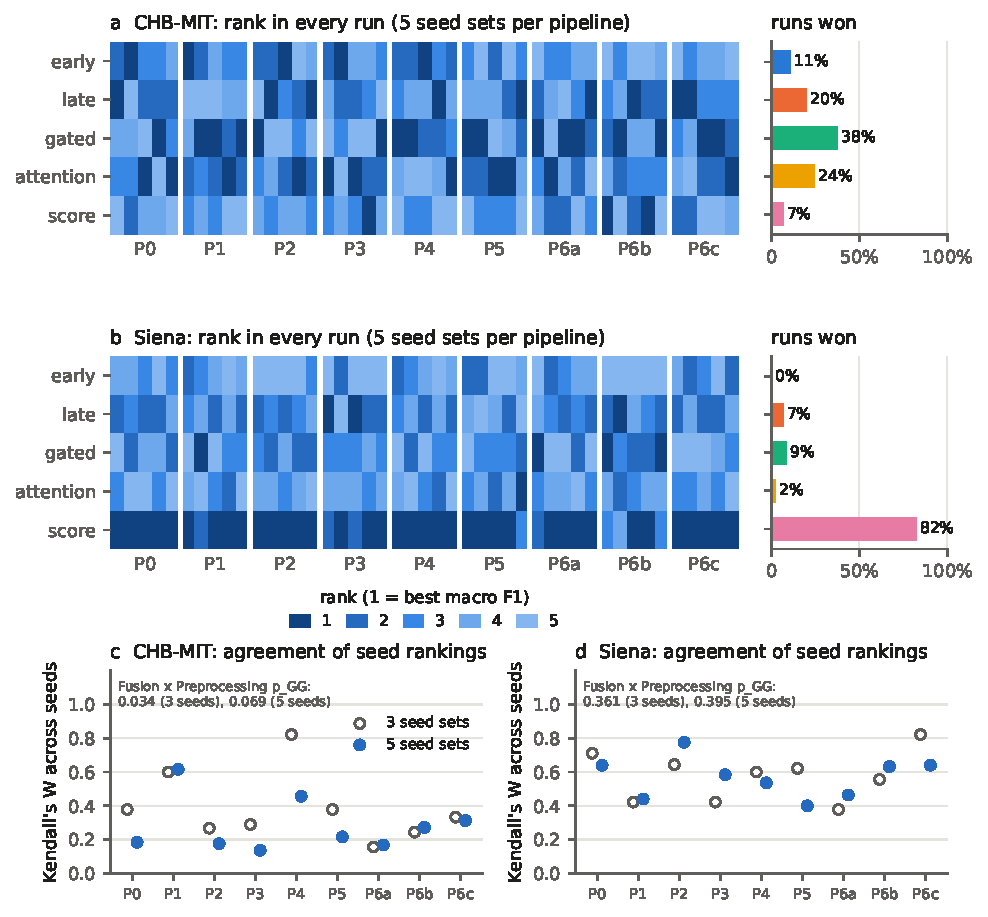
\includegraphics[width=1\linewidth,height=\textheight,keepaspectratio,alt={Ranking stability. a, b, Rank of each operator by macro F1 in every run (within each pipeline, one column per seed set; darker is better), and the share of the 45 runs of each dataset in which the operator ranked first. c, d, Agreement of the operator rankings across seed sets within each pipeline (Kendall's W) with three and with five seed sets, and the Greenhouse-Geisser-corrected p of the Fusion × Preprocessing interaction with each.}]{figure4_rank_stability.pdf}
\caption{Ranking stability. \textbf{a, b}, Rank of each operator by macro F1 in every run (within each pipeline, one column per seed set; darker is better), and the share of the 45 runs of each dataset in which the operator ranked first. \textbf{c, d}, Agreement of the operator rankings across seed sets within each pipeline (Kendall's W) with three and with five seed sets, and the Greenhouse-Geisser-corrected p of the Fusion × Preprocessing interaction with each.}\label{fig:4}
\end{figure}

\subsection{3.4 Subject heterogeneity dominates the variability due to model and preprocessing choices}\label{subject-heterogeneity-dominates-the-variability-due-to-model-and-preprocessing-choices}

To identify the factors behind the variability, each metric was decomposed into
subject, operator, preprocessing, seed and interaction components (Figure 5a, b).

On CHB-MIT the held-out subject accounted for 74.2 percent of the variance of macro F1
(SD 0.126), its interactions with pipeline and operator for 7.2 percent and the residual
for 17.3 percent. All seed terms together accounted for 1.1 percent (SD 0.015), more
than the operator and preprocessing, whose estimates were below zero (-2.4e-5 and
-2.7e-5), that is, below their error terms (a zero share means that these effects
could not be separated from their error terms, not that they are absent); the Fusion × Preprocessing component was
0.09 percent, consistent with the small practical size of the interaction despite its
sensitivity to the number of seeds. AUPRC (subject 76.8 percent, operator 0.8, seed 1.5)
and balanced accuracy (72.9, 0, 1.4) showed the same structure. Preprocessing had no
detectable main effect in the repeated-measures ANOVA either (F = 0.29, Greenhouse-Geisser
p = 0.83, partial eta squared 0.013).

On Siena the variability was more distributed. The subject accounted for 32.5 percent and
its interactions with pipeline and operator for a further 26.9 percent; the operator
held 1.5 percent of the variance of macro F1 (SD 0.016) and 5.5 percent of AUPRC, the seed
4.2 percent and preprocessing 0.06 percent (main effect F = 1.09, p = 0.36).

The effects of fusion and preprocessing therefore cannot be characterised by their
dataset-level averages alone. Mean macro F1 per held-out subject ranged from 0.46
(chb05) to 0.87 (chb22) on CHB-MIT and from 0.51 (PN07) to 0.78 (PN00) on Siena
(Figure 5c, d). Within a subject the operators differed by a median of 0.063 macro F1 on
CHB-MIT and 0.10 on Siena, three and two times the median difference within a pipeline,
and the best operator changed from subject to subject: on CHB-MIT each of the five
operators was the best for at least two subjects. An operator that suits one subject
often does not suit another. This heterogeneity also explains why small differences in
mean macro F1 were difficult to establish statistically: with 23 subjects on CHB-MIT and
14 on Siena, the uncertainty of every comparison is dominated by the variation between
held-out subjects. The variance decomposition thus identifies subject heterogeneity as a
central feature of the benchmark rather than as residual noise.

\begin{figure}
\centering
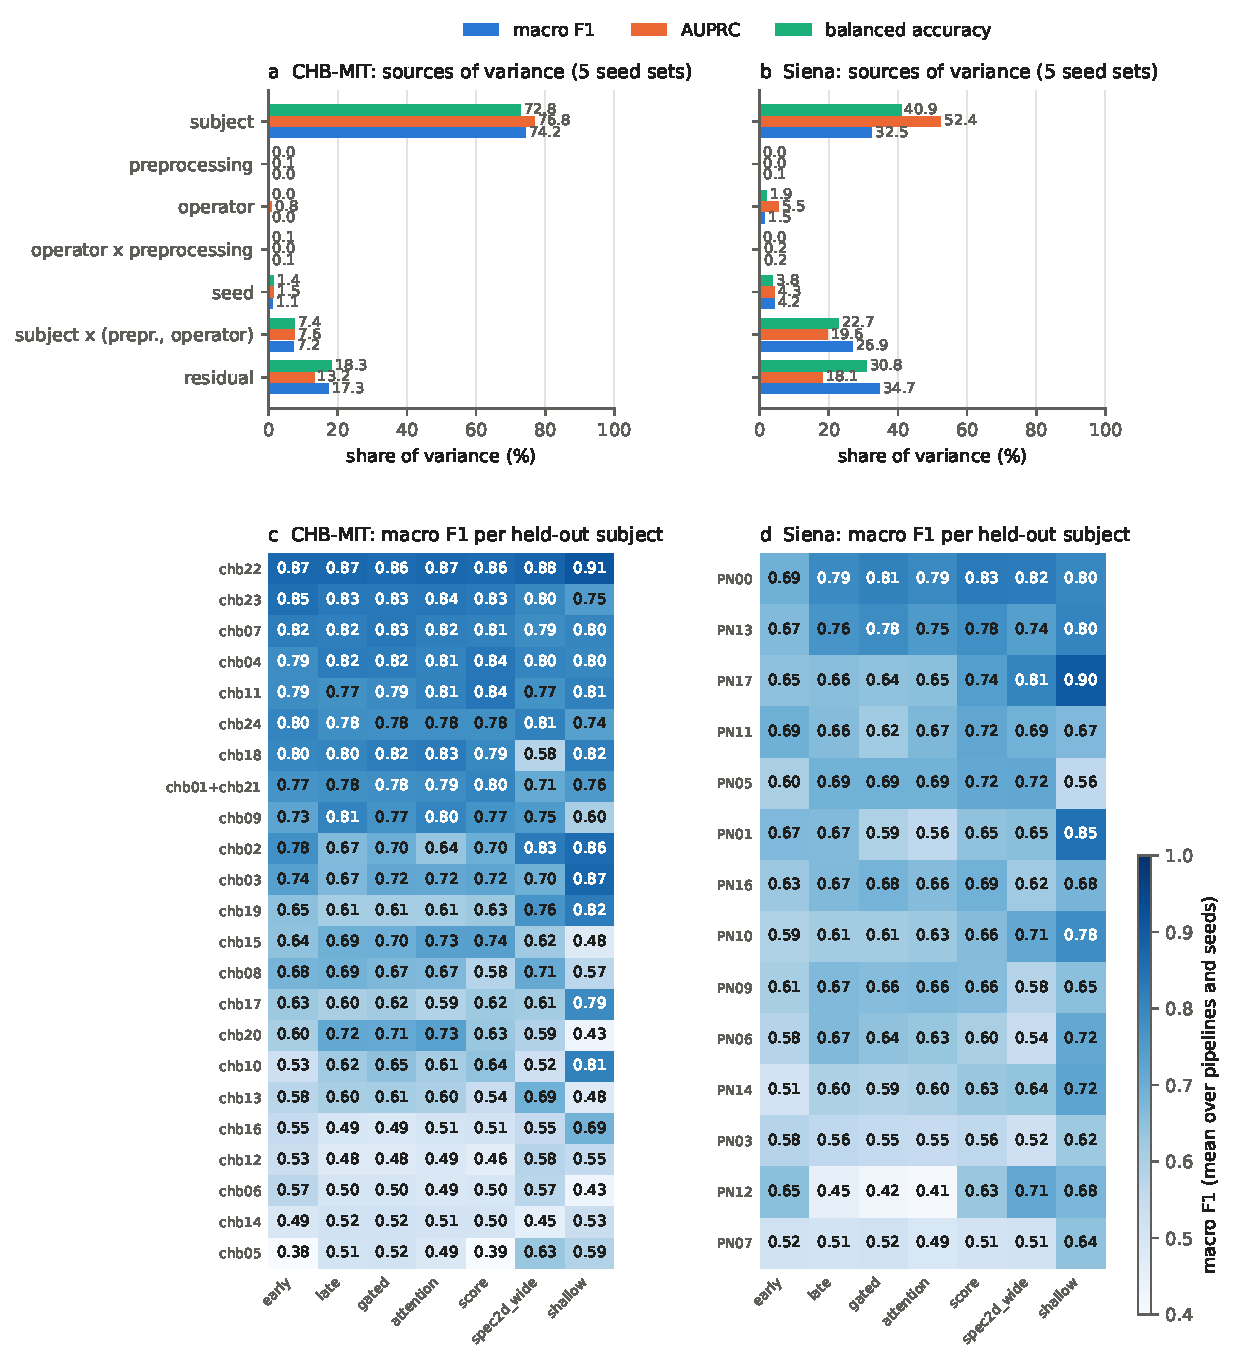
\includegraphics[width=1\linewidth,height=\textheight,keepaspectratio,alt={Sources of variability. a, b, Shares of the variance of macro F1, AUPRC and balanced accuracy (method-of-moments estimates for a fully crossed random-effects model of subject, preprocessing, operator and seed; negative estimates shown as 0; seed: all seed terms together). c, d, Macro F1 per held-out subject and model, mean over the nine pipelines and five seed sets; subjects sorted by their mean over the models.}]{figure5_variance.pdf}
\caption{Sources of variability. \textbf{a, b}, Shares of the variance of macro F1, AUPRC and balanced accuracy (method-of-moments estimates for a fully crossed random-effects model of subject, preprocessing, operator and seed; negative estimates shown as 0; seed: all seed terms together). \textbf{c, d}, Macro F1 per held-out subject and model, mean over the nine pipelines and five seed sets; subjects sorted by their mean over the models.}\label{fig:5}
\end{figure}

\subsection{3.5 Artefact removal involves trade-offs between signal preservation, performance, cost and reproducibility}\label{artefact-removal-involves-trade-offs-between-signal-preservation-performance-cost-and-reproducibility}

The three artefact removal procedures (Extended Infomax, GEDAI and AMICA) were evaluated
for their effect on classification and also for signal preservation, computational cost
and reproducibility (Figure 6).

Infomax and AMICA removed a median of one component per recording and kept a median of
78 percent of the signal's power; GEDAI kept 99.9 percent in most recordings but removed
more than half of the power in 21 percent of them. They differed strongly in cost:
cleaning the 670 CHB-MIT recordings took 8.5 CPU hours with Infomax, 4.7 with GEDAI and
73 with AMICA. Infomax and AMICA removed mostly delta power and, within a recording,
slightly less from ictal than from non-ictal windows (a median difference of 0.010 and
0.017 of the power kept, Wilcoxon p \textless{} 0.001). Over the whole corpus, GEDAI's default
preset kept a median of 63 percent of the power of CHB-MIT's ictal windows against 93
percent of the non-ictal ones, because the recordings it cleaned heavily held many of the
seizures; within recordings it showed no difference (Supplementary Table S5).

The effect on classification was not uniform across operators or datasets. Against P1,
the same signal without artefact removal, late fusion gained 0.014 to 0.022 macro F1 on
CHB-MIT under all three algorithms and early fusion lost 0.012 to 0.022; on Siena GEDAI
raised late and gated fusion by 0.045 and 0.061. AUPRC fell under every algorithm for most
operators, by up to 0.060 (early fusion under GEDAI, CHB-MIT). No algorithm was better
than the others for every operator and setting.

A separate analysis showed that the procedures differed in reproducibility (Section 2.7).
With the same code, package versions and seeds, GEDAI cleaned about 27 percent of
recordings differently on a second machine. Extended Infomax removed different
components in about 2.5 percent of recordings between machines and in about 1.2 percent
between two runs on the same machine with different process parallelism. AMICA removed
the same components in every recording on both machines, and its retained power differed
by at most 0.003. Experiments with a third machine of another architecture and with
rounding-level perturbations of the input suggest that some cleaning decisions are
sensitive to floating-point variation near the algorithms' decision thresholds.

These differences were not confined to intermediate signals. Scoring the same trained
models on recordings cleaned on two machines changed seizure-level sensitivity by up to
0.054 under GEDAI and changed the order of the operators by sensitivity (Kendall tau 0.60
to 1.00); the change was at most 0.005 under Infomax and absent under AMICA.
Reproducibility at the level of code, package versions and seeds therefore did not
guarantee reproducible cleaned signals or downstream predictions. The results identify a
trade-off: an inexpensive cleaning method can introduce more variation between machines,
whereas a costlier one can give more stable outputs, and the reproducibility of
preprocessing can affect the conclusions of a model comparison.

\begin{figure}
\centering
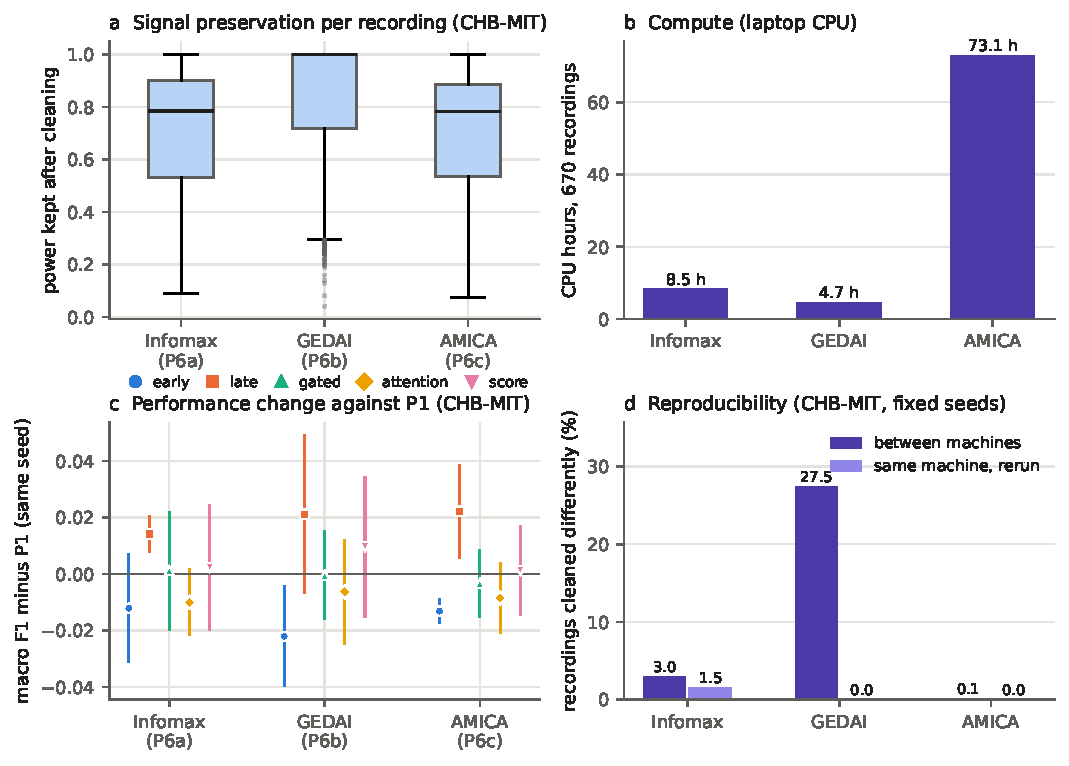
\includegraphics[width=1\linewidth,height=\textheight,keepaspectratio,alt={Artefact removal in P6 (CHB-MIT). a, Share of each recording's power kept after cleaning (670 recordings). b, CPU hours for the 670 recordings on a laptop CPU. c, Change in macro F1 against P1, the same 0.5 to 40 Hz signal without artefact removal, paired by seed set; mean and SD over five seed sets. d, Share of recordings cleaned differently (different components removed, or retained power differing by more than 0.001) on a second machine and in a second run on the same machine, with the same code, package versions and seeds.}]{figure6_artefact_removal.pdf}
\caption{Artefact removal in P6 (CHB-MIT). \textbf{a}, Share of each recording's power kept after cleaning (670 recordings). \textbf{b}, CPU hours for the 670 recordings on a laptop CPU. \textbf{c}, Change in macro F1 against P1, the same 0.5 to 40 Hz signal without artefact removal, paired by seed set; mean and SD over five seed sets. \textbf{d}, Share of recordings cleaned differently (different components removed, or retained power differing by more than 0.001) on a second machine and in a second run on the same machine, with the same code, package versions and seeds.}\label{fig:6}
\end{figure}

\subsection{3.6 Window-level differences translate into different seizure-level operating points}\label{window-level-differences-translate-into-different-seizure-level-operating-points}

The window-level analysis was complemented by seizure-level evaluation on the complete
recordings, with the probability threshold of 0.5 fixed in advance and without
post-processing (Figure 7).

On CHB-MIT the operators detected 68 to 79 percent of the annotated seizures, with 5.2 to
7.7 false alarms per hour (\nolinkurl{results_v2/results/events_chbmit.csv}). Early fusion had a
distinct operating point: it reached the highest mean seizure-level sensitivity (0.79)
and ranked first in sensitivity in 82 percent of runs, but it also raised the most false
alarms in every run (7.7 per hour against 5.2 to 5.7 for the other operators). Taken
together with the window-level results, in which early fusion had the lowest AUPRC in
every pipeline of both datasets, this shows that a higher sensitivity at a given
threshold does not imply better discrimination: early fusion labels more windows ictal,
which detects more seizures at the price of more false alarms.

Artefact removal did not remove this trade-off. Under Infomax and AMICA the operators
detected 66 to 76 percent of seizures with 4.8 to 7.2 false alarms per hour; under GEDAI,
71 to 80 percent with 5.5 to 8.7. On Siena the operators detected 84 to 87 percent of
seizures, without a consistent order; false alarms per hour are not reported for Siena
because its recordings are cut around the seizures and do not represent continuous
monitoring.

Small differences in window-level macro F1 can therefore coexist with clearly different
balances between seizure sensitivity and false-alarm burden, and window-level
classification metrics alone do not characterise how a seizure detector would operate.

\begin{figure}
\centering
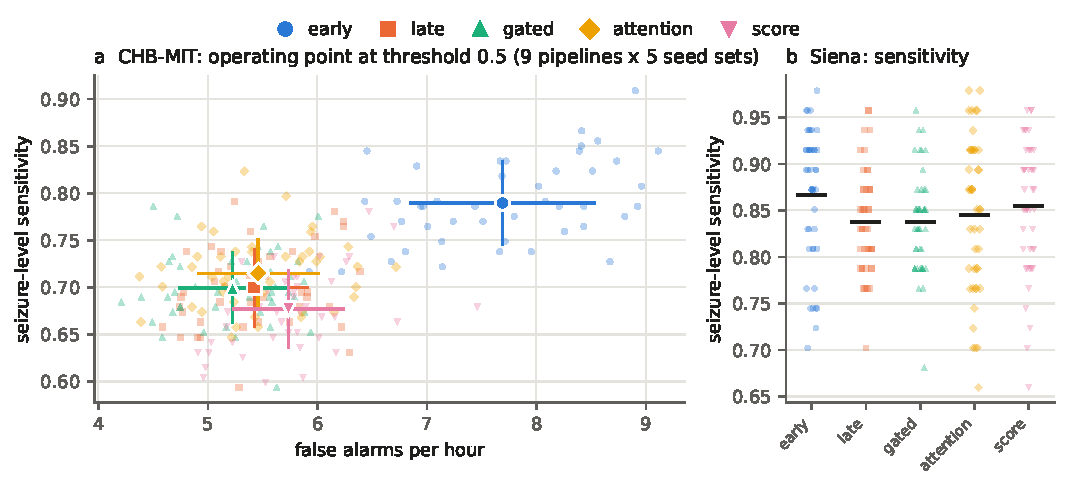
\includegraphics[width=1\linewidth,height=\textheight,keepaspectratio,alt={Seizure-level detection at the fixed threshold of 0.5 without post-processing. a, CHB-MIT: sensitivity against false alarms per hour, one point per run (nine pipelines × five seed sets) and the operator's mean and SD. b, Siena: seizure-level sensitivity per operator, one point per run, with the mean as a bar; false alarms per hour are not reported for Siena.}]{figure7_seizure_level.pdf}
\caption{Seizure-level detection at the fixed threshold of 0.5 without post-processing. \textbf{a}, CHB-MIT: sensitivity against false alarms per hour, one point per run (nine pipelines × five seed sets) and the operator's mean and SD. \textbf{b}, Siena: seizure-level sensitivity per operator, one point per run, with the mean as a bar; false alarms per hour are not reported for Siena.}\label{fig:7}
\end{figure}

\subsection{3.7 Predictive performance transfers across datasets, but operator rankings do not}\label{predictive-performance-transfers-across-datasets-but-operator-rankings-do-not}

Finally, we examined whether the patterns observed in subject-independent evaluation
generalise across datasets (Figure 8).

Models trained on all of CHB-MIT and tested on Siena reached a mean macro F1 of 0.641
(attention) to 0.677 (late) over pipelines and seed sets. For early, late, gated and
attention fusion this was higher than the mean obtained by training and testing on Siena
(LOSO); score fusion was the exception, with 0.652 after transfer against 0.670 within
Siena.

Comparable aggregate performance did not mean that the order of the operators carried
over. Score fusion, first in 82 percent of Siena's own runs, was first in 11 percent of
the transfer runs; there, late fusion ranked first most often (38 percent) and attention
fusion was most often last (40 percent). Kendall tau between the seed-averaged operator
rankings of the same pipeline was -0.11 on average between CHB-MIT and Siena, 0.07
between CHB-MIT and the transfer, and -0.11 between Siena and the transfer.

These results distinguish two forms of generalisation: whether a trained model keeps
useful performance on an independent dataset, and whether the advantage of one fusion
operator over another is preserved. The former was observed at the level of aggregate
macro F1, the latter was not; an operator that ranked highly when trained and evaluated
on one dataset did not necessarily keep that position under external evaluation.

\begin{figure}
\centering
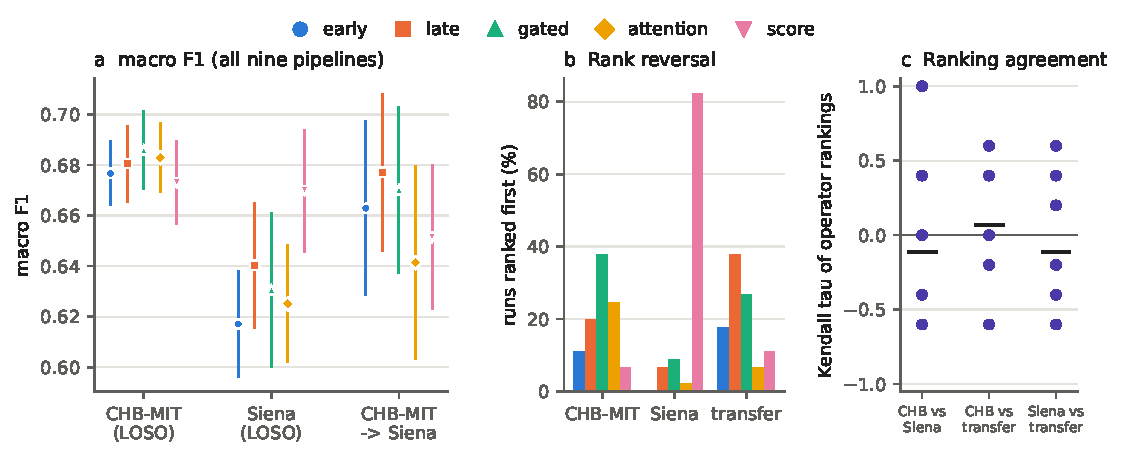
\includegraphics[width=1\linewidth,height=\textheight,keepaspectratio,alt={Cross-dataset generalisation. a, Macro F1 of each operator on CHB-MIT (LOSO), on Siena (LOSO), and trained on CHB-MIT and tested on Siena; mean and SD over the runs of all nine pipelines and five seed sets. b, Share of runs in which each operator ranks first in each setting. c, Kendall tau between the seed-averaged operator rankings of the same pipeline in two settings; one point per pipeline (points can overlap), bar: mean.}]{figure8_cross_dataset.pdf}
\caption{Cross-dataset generalisation. \textbf{a}, Macro F1 of each operator on CHB-MIT (LOSO), on Siena (LOSO), and trained on CHB-MIT and tested on Siena; mean and SD over the runs of all nine pipelines and five seed sets. \textbf{b}, Share of runs in which each operator ranks first in each setting. \textbf{c}, Kendall tau between the seed-averaged operator rankings of the same pipeline in two settings; one point per pipeline (points can overlap), bar: mean.}\label{fig:8}
\end{figure}

\section{4. Discussion}\label{discussion}

We asked whether conclusions about fusion operators for EEG seizure detection hold when
the preprocessing, the artefact removal algorithm, the training seed and the dataset
change. On both datasets the answer is largely no: the operators performed within a few
hundredths of macro F1 of each other, no difference between them was significant, and
their order changed with the seed, with the artefact removal algorithm on Siena, and
between datasets. We take the advisor's questions in turn.

\subsection{4.1 How large are the differences between fusion operators?}\label{how-large-are-the-differences-between-fusion-operators}

Small. Within a pipeline the best and worst operator differed by a median of 0.021
macro F1 on CHB-MIT and 0.053 on Siena, and no pairwise difference survived the
corrected test. The operator's share of the variance was estimated below zero on
CHB-MIT and at 1.5 percent on Siena. One operator did stand apart in one respect: early
fusion ranked windows by ictal probability worst in every pipeline of both datasets
(lowest AUPRC in 18 of 18 cases), while its thresholded macro F1 was unremarkable and
its seizure-level sensitivity, at the price of more false alarms, the highest. Early
fusion is the only operator that combines the two representations before either branch
has learned its own features, and its weaker ranking of windows is the one property of
an operator that the multiverse preserved. Whether two operators are \emph{equivalent} is a
separate question, and the answer depends on the dataset: on CHB-MIT most pairs were
equivalent within 0.05 macro F1 in most pipelines and two in all, but within 0.02 almost
none, and on Siena few were equivalent even within 0.05. The data therefore rule out
large differences between operators on CHB-MIT, but not differences of the size that
published comparisons typically report as improvements.

The controls put these differences in proportion (Section 3.1, Table 4, Figure 2). A
single-branch spectrogram network of the same size had a mean macro F1 similar to
that of the jointly trained operators on CHB-MIT and higher on Siena, and a logistic
regression on seven hand-crafted features had a mean macro F1 as high as or higher than
every network, though not a higher AUPRC on CHB-MIT. Under the corrected test none of these
differences was significant, nor was the higher mean AUPRC of the fused models on
CHB-MIT, and few were demonstrably equivalent: the controls stand to the operators as
the operators stand to each other. Fusing the two representations may help the ranking
of windows, by about as much as the operators differed from each other on CHB-MIT, but
neither the choice to fuse nor the choice of operator changed performance as much as
the subject did. This agrees with a broader evaluation of
multimodal models, available as a preprint, in which added fusion complexity often did
not pay off (\citealp{Rheude_2025}). An improvement of one fusion operator over
another says little without a parameter-matched unimodal control and a simple classical
baseline evaluated in the same way.

\subsection{4.2 Are the differences preserved when preprocessing changes?}\label{are-the-differences-preserved-when-preprocessing-changes}

Preprocessing had no detectable main effect on performance and did not reorder the
operators more than a change of seed did. The interaction between operator and
preprocessing, significant with three seed sets on CHB-MIT, was no longer significant
after correction with five (p = 0.069), and its variance component was 0.09 percent. The
one place where preprocessing mattered more than the seed was the choice among the three
artefact removal algorithms on Siena (p = 0.029), where GEDAI raised late and gated
fusion by about 0.05 macro F1. This agrees with the wider literature, where
preprocessing changes results but no pipeline is best throughout (Section 1.1), and it
adds that, for a comparison of operators, the pipeline mostly adds noise rather than a
systematic advantage for one operator.

\subsection{4.3 How much does the random seed change the rankings?}\label{how-much-does-the-random-seed-change-the-rankings}

More than preprocessing does. On CHB-MIT the rankings from five seeds of the same
pipeline agreed barely above chance (median Kendall's W 0.22), all seed terms together
explained more of the variance than preprocessing and the operator, and the
window-level predictions changed as much between seeds as between pipelines. A ranking
obtained from one training run is therefore close to a random draw on CHB-MIT. The
consequence for the literature is direct: a comparison of operators that reports one run
per operator, as most do, cannot distinguish a better operator from a lucky seed at the
differences observed here. Five seeds were enough to show this, and gave a more reliable
estimate of the Fusion x Preprocessing interaction than three: significant with three
seed sets, it was not with five (Section 3.3). That the seed explains more variance than
the pipeline, shown with five seed sets, is a direct caution for the many comparisons
that report a single run.

\subsection{4.4 Why does the subject dominate?}\label{why-does-the-subject-dominate}

Subject-associated variability made up 74 percent of the variance on CHB-MIT and,
together with its interactions with pipeline and operator, about 60 percent on Siena. Seizures differ
between people in morphology, location and duration, and the recordings in their
equipment, montage quality and artefacts; a model trained on the other subjects works
well or badly on a given person largely for reasons that no fusion operator or
preprocessing step changes. The interaction of subject with pipeline and operator, 7
percent on CHB-MIT and 27 percent on Siena, means that the operator that suits one
person is often not the one that suits another. Averaging over subjects hides this
heterogeneity, and with 23 and 14 subjects it also limits the precision of every
comparison between operators: the equivalence bounds of Section 3.2 are as wide as they
are because the subjects differ so much.

\subsection{4.5 Does the choice of artefact removal algorithm affect reliability?}\label{does-the-choice-of-artefact-removal-algorithm-affect-reliability}

In two ways. The three algorithms changed performance differently by operator
(Section 3.5), and on Siena they reordered the operators more than the seed did. Less
expected, they differed in reproducibility. With the same code, package versions and
seeds, GEDAI cleaned about a quarter of recordings differently on a second machine, and
Infomax changed its component decision in 2.5 percent of recordings between machines
and in about 1 percent between two runs on one machine; scoring the same trained models on the two cleanings changed seizure-level
sensitivity by up to 0.054 and the order of the operators. Fixed seeds and pinned
versions are the reproducibility measures a methods section usually reports; for
ICA-based cleaning they were not sufficient here, plausibly because decisions made at
a threshold (a component's \textbar z\textbar{} against an EOG proxy, GEDAI's noise threshold) amplify
rounding differences between machines. A perturbation of the input of one part in ten million
produced differences of the same kind, which suggests that no machine gives the
correct result and that choosing a different machine would not avoid them. The window-level results of this study rest on one
cleaning and are unaffected; but a study that cleans its training data on one machine
and its test data on another, or that compares its numbers with another group's, can
see differences of the size of the effect it studies. Neuroimaging pipelines, including ICA decompositions of fMRI
data, are known to give different results on different operating systems (\citealp{Glatard_2015}); we are not aware of a comparable report for EEG artefact removal, where
algorithms that take threshold decisions near floating-point precision can be
deterministic within a machine (GEDAI) or even within one execution context (Infomax)
and still not reproducible across machines. We recommend that studies using
artefact removal store the cleaned signals, or at least the decomposition and the
removed components, alongside the code.

\subsection{4.6 Do results from one dataset carry over to another?}\label{do-results-from-one-dataset-carry-over-to-another}

Performance did, rankings did not. Models trained on CHB-MIT reached on Siena the macro
F1 of models trained on Siena itself, but the order of the operators on CHB-MIT, on
Siena and after transfer were unrelated (mean Kendall tau between -0.11 and 0.07). Score
fusion is the clearest case: first in 82 percent of Siena's own runs, it was first in 11
percent of the transfer runs and among the weaker operators on CHB-MIT. Its advantage on
Siena is therefore a property of training and testing on Siena, not a property of the
operator. Part of it is inherited from its spectrogram branch: on Siena the
spectrogram network alone (0.660 macro F1) already had a higher mean than every
jointly trained operator, and score fusion averages it with the waveform network, with a weight chosen
on Siena's validation subjects. Whether end-to-end training of the joint operators
overfits Siena's 14 subjects, which training the branches independently would avoid,
we did not test. The two datasets differ in age, seizure types, recording protocol and mains
frequency (Section 2.1), so we do not attribute the difference to any one of these.

\subsection{4.7 Statistical significance, practical size and ranking stability}\label{statistical-significance-practical-size-and-ranking-stability}

The three properties we kept apart gave different answers, and reporting any one alone
would have misled. On Siena score fusion was first in four of five runs, a stable
ranking, yet its advantage was not significant and could not be shown to exceed or fall
below 0.05 macro F1. On CHB-MIT the interaction was significant before correction and
with three seeds, yet its practical size was 0.004 macro F1. And on CHB-MIT several pairs
of operators were practically equivalent while their order changed from seed to seed,
which is what equivalence implies: when two operators are equally good, their order is
decided by noise. A stable ranking is not evidence of a meaningful difference, a
significant effect is not evidence of a large one, and the absence of a significant
difference is not evidence of equivalence.

\subsection{4.8 What this means for comparisons of fusion operators}\label{what-this-means-for-comparisons-of-fusion-operators}

We did not find a fusion operator that is better than the others across preprocessing,
seeds and datasets, and our results do not support claims that one is. That is itself
the main finding: a claim of superiority based on one dataset, one pipeline and one
training run, the common design in this literature, would have reached a different
conclusion in different runs of our study. Comparisons of this kind should report
several seeds and, where feasible, several preprocessing choices; test differences with
corrected and equivalence tests rather than naive paired tests; report the rank
distribution rather than one ranking; include a parameter-matched unimodal control and
a simple classical baseline; and state the margin below which a difference is
considered irrelevant before looking at the results.

\subsection{4.9 What do the results mean clinically?}\label{what-do-the-results-mean-clinically}

\emph{(Draft. All nine pipelines on CHB-MIT, five seed sets each.)}

None of the systems studied here is close to clinical use, and the study was not
designed to produce one: the threshold was fixed at 0.5, there was no post-processing,
and the models were trained on other people's seizures only. At that operating point
the operators detected 68 to 79 percent of CHB-MIT's seizures with 5.2 to 7.7 false
alarms per hour, that is 125 to 185 false alarms per day of monitoring, and about 2
percent of all detections were seizures. Generic scalp EEG detectors evaluated for
clinical use have reported 0.1 to 5 false alarms per hour, most about 0.2 to 0.3, and
patient-specific detectors fewer, and a low false alarm rate is regarded as essential
for clinical acceptance, and validation standards require it to be reported
(\citealp{Baumgartner_2018}; \citealp{Beniczky_2018}); no person in CHB-MIT reached a mean below one false alarm per hour.
The detection threshold trades sensitivity against false alarms, and training or
adjusting the detector per patient lowers the false alarm rate (\citealp{Baumgartner_2018}): patient-specific classifiers detected 96 percent of the CHB-MIT seizures with a
median of two false detections per day (\citealp{Shoeb_2010}). We left per-patient
thresholds and post-processing of consecutive windows out on purpose, so that the operators are compared on their
raw output, and the absolute numbers should be read in that light. The criteria were
fixed before the runs; choosing a threshold or a post-processing rule after seeing the
results would select the criterion on the outcome.

Three results nevertheless bear on clinical use. First, the operators that differed by
a few hundredths of macro F1 at the window level differed by little more at the seizure
level, except early fusion, which detected the most seizures (0.79) at the most false
alarms (7.7 per hour); which of these is preferable is a clinical choice between missed
seizures and alarm fatigue (\citealp{Sendelbach_2013}), not a property that window-level
metrics reveal.
Second, the person mattered more than any modelling choice: mean sensitivity ranged
from 0.24 (chb06) to 1.00 across persons and the false alarm rate from 1.3 to 12.3 per
hour, while the operators' means spanned 0.68 to 0.79 and 5.2 to 7.7. For a patient,
whether the detector works depends far more on who they are than on the fusion
operator, which supports patient-specific adaptation over the search for a better
generic operator (\citealp{Shoeb_2010}; \citealp{Baumgartner_2018}). Third, an artefact removal step that does not reproduce across
machines (Section 4.5) is a clinical risk as much as a scientific one: the same model
could detect a different set of a patient's seizures depending on where the recording
is cleaned.

Siena cannot answer the clinical question of false alarms: its recordings are cut
around seizures, so we report only its sensitivity (84 to 87 percent), which is
consistent with CHB-MIT's and says nothing about specificity in continuous monitoring.
Neither dataset contains the long, artefact-rich ambulatory or intensive-care
recordings in which seizure detectors are used, and the persons are few (23 and 14).

\subsection{4.10 Limitations}\label{limitations}

\emph{(draft; to be completed with the results)}

\begin{itemize}
\tightlist
\item
  \textbf{Sample size.} Twenty-three CHB-MIT and fourteen Siena subjects make the corrected
  confidence intervals wide: differences between operators that are small can be neither
  shown nor excluded at the equivalence margins, so many pairs are neither different nor
  demonstrably equivalent.
\item
  \textbf{One design family.} All operators share one pair of representations (raw waveform
  and log-magnitude STFT), one backbone family and one parameter budget; other
  representations (wavelets, other time-frequency transforms) or larger models may
  behave differently. Widening a single branch to the fusion budget did not change its
  performance (Section 3.1), but deeper backbones were not tested.
\item
  \textbf{Windows, not sessions.} Window-level metrics use non-ictal windows subsampled to
  four per ictal window, so they do not reflect the true prevalence of seizures; the
  seizure-level metrics on the full recordings address this but are secondary. A window
  is labelled ictal if it overlaps a seizure at all; excluding partly ictal windows is
  implemented but was not run.
\item
  \textbf{Siena.} Its recordings are cut around seizures, so false alarms per hour cannot be
  interpreted and are not reported; the summed recording time (141.0 h by the EDF
  headers) differs from the dataset description (128.4 h) for reasons that remain
  unexplained for three patients. Six problems in its seizure lists were resolved by
  decisions documented in Supplementary Table S4.
\item
  \textbf{CHB-MIT.} Thirteen of its 198 seizures lie in recordings without the standard
  montage and are not used; chb24 is not listed in the subject information file and is
  treated as a distinct person.
\item
  \textbf{Artefact removal.} The settings (16 components, frontopolar channels as EOG proxies,
  no muscle rejection) and the projection of GEDAI's reference onto a bipolar montage are
  our choices for montages without EOG; GEDAI was designed for referential, high-density
  recordings. That Infomax's and GEDAI's results do not reproduce across machines is a
  finding of this study (Sections 2.7 and 4.5); for its own results, window-level
  metrics rest on one cleaning, but the seizure-level metrics of P6a
  differ from the training-time cleaning in 8 of 670 recordings.
\item
  \textbf{Device.} All multiverse runs used one GPU; GPU and CPU results at the same seeds
  differ by an amount comparable to the difference between seed sets, so absolute
  numbers are not interchangeable with the CPU results of earlier drafts.
\item
  \textbf{Offline processing.} Filters and artefact cleaning see the complete recording
  (Section 2.2), so the results describe offline preprocessing, not a causal, real-time
  detector.
\item
  \textbf{No tuning.} One fixed training configuration was used for every model; an operator
  might gain more than another from tuning, which this design does not test.
\item
  \textbf{Two datasets.} CHB-MIT and Siena differ in population, acquisition and recording
  protocol at once, so the transfer experiment measures their combined shift and cannot
  attribute a change in performance or ranking to any one of these differences.
\item
  \textbf{Seeds.} Five seed sets bound the seed variance only roughly; the rank analyses
  report it rather than average it away.
\item
  \textbf{Literature.} Title and abstract screening of the systematic search was done by an
  AI assistant (agreement with an independent AI pass, kappa 0.81); a human screening
  and the full texts of the remaining candidates are in progress, and claims marked
  {[}abstract{]} in Section 1 rest on abstracts.
\end{itemize}

\section{Use of AI assistance}\label{use-of-ai-assistance}

The authors acknowledge the use of AI-supported language editing, structuring and
coding assistance (Claude, Anthropic) during manuscript preparation. The authors remain
fully responsible for the data, analysis, interpretation, and final text.

\bibliographystyle{plainnat}
\bibliography{main}

\clearpage
\section*{Supplementary Material}
\setcounter{table}{0}
\renewcommand{\thetable}{S\arabic{table}}
\renewcommand{\theHtable}{S\arabic{table}}
\setcounter{figure}{0}
\renewcommand{\thefigure}{S\arabic{figure}}
\renewcommand{\theHfigure}{S\arabic{figure}}

\begingroup\footnotesize\setlength{\tabcolsep}{3pt}

\begin{longtable}[]{@{}
  >{\raggedright\arraybackslash}p{(\linewidth - 16\tabcolsep) * \real{0.1493}}
  >{\raggedright\arraybackslash}p{(\linewidth - 16\tabcolsep) * \real{0.1095}}
  >{\raggedright\arraybackslash}p{(\linewidth - 16\tabcolsep) * \real{0.1095}}
  >{\raggedright\arraybackslash}p{(\linewidth - 16\tabcolsep) * \real{0.1144}}
  >{\raggedright\arraybackslash}p{(\linewidth - 16\tabcolsep) * \real{0.0746}}
  >{\raggedright\arraybackslash}p{(\linewidth - 16\tabcolsep) * \real{0.0896}}
  >{\raggedright\arraybackslash}p{(\linewidth - 16\tabcolsep) * \real{0.1244}}
  >{\raggedright\arraybackslash}p{(\linewidth - 16\tabcolsep) * \real{0.1294}}
  >{\raggedright\arraybackslash}p{(\linewidth - 16\tabcolsep) * \real{0.0995}}@{}}
\caption{\textbf{Artefact removal in P6: signal retention and compute.} Per recording of CHB-MIT with selected windows (670), on the 0.5 to 40 Hz signal. Power kept = signal power after removal / before. Extended Infomax and AMICA share 16 components, fitting on every 8th sample and the same automatic ocular component rule; GEDAI selects what to remove by its own criterion. Compute on a laptop CPU (Intel Core Ultra 7 155U), six recordings in parallel.}\tabularnewline
\toprule\noalign{}
\begin{minipage}[b]{\linewidth}\raggedright
method
\end{minipage} & \begin{minipage}[b]{\linewidth}\raggedright
recordings
\end{minipage} & \begin{minipage}[b]{\linewidth}\raggedright
power kept, median
\end{minipage} & \begin{minipage}[b]{\linewidth}\raggedright
IQR
\end{minipage} & \begin{minipage}[b]{\linewidth}\raggedright
min
\end{minipage} & \begin{minipage}[b]{\linewidth}\raggedright
share \textless{} 0.5
\end{minipage} & \begin{minipage}[b]{\linewidth}\raggedright
components removed, mean
\end{minipage} & \begin{minipage}[b]{\linewidth}\raggedright
seconds per recording, median
\end{minipage} & \begin{minipage}[b]{\linewidth}\raggedright
CPU hours, total
\end{minipage} \\
\midrule\noalign{}
\endfirsthead
\toprule\noalign{}
\begin{minipage}[b]{\linewidth}\raggedright
method
\end{minipage} & \begin{minipage}[b]{\linewidth}\raggedright
recordings
\end{minipage} & \begin{minipage}[b]{\linewidth}\raggedright
power kept, median
\end{minipage} & \begin{minipage}[b]{\linewidth}\raggedright
IQR
\end{minipage} & \begin{minipage}[b]{\linewidth}\raggedright
min
\end{minipage} & \begin{minipage}[b]{\linewidth}\raggedright
share \textless{} 0.5
\end{minipage} & \begin{minipage}[b]{\linewidth}\raggedright
components removed, mean
\end{minipage} & \begin{minipage}[b]{\linewidth}\raggedright
seconds per recording, median
\end{minipage} & \begin{minipage}[b]{\linewidth}\raggedright
CPU hours, total
\end{minipage} \\
\midrule\noalign{}
\endhead
\bottomrule\noalign{}
\endlastfoot
P6a Extended Infomax & 670 & 0.784 & 0.531-0.899 & 0.090 & 0.222 & 1.491 & 33 & 8.5 \\
P6b GEDAI, conservative (used) & 670 & 0.999 & 0.717-0.999 & 0.041 & 0.206 & & 18 & 4.7 \\
P6c AMICA & 670 & 0.784 & 0.535-0.885 & 0.076 & 0.228 & 1.531 & 213 & 73.1 \\
GEDAI, default (not used) & 670 & 0.658 & 0.317-0.999 & 0.041 & 0.433 & & 22 & 5.6 \\
\end{longtable}

\endgroup

\begingroup\footnotesize

\begin{longtable}[]{@{}
  >{\raggedright\arraybackslash}p{(\linewidth - 16\tabcolsep) * \real{0.1759}}
  >{\raggedright\arraybackslash}p{(\linewidth - 16\tabcolsep) * \real{0.1407}}
  >{\raggedright\arraybackslash}p{(\linewidth - 16\tabcolsep) * \real{0.0905}}
  >{\raggedright\arraybackslash}p{(\linewidth - 16\tabcolsep) * \real{0.0905}}
  >{\raggedright\arraybackslash}p{(\linewidth - 16\tabcolsep) * \real{0.0905}}
  >{\raggedright\arraybackslash}p{(\linewidth - 16\tabcolsep) * \real{0.1005}}
  >{\raggedright\arraybackslash}p{(\linewidth - 16\tabcolsep) * \real{0.0905}}
  >{\raggedright\arraybackslash}p{(\linewidth - 16\tabcolsep) * \real{0.1106}}
  >{\raggedright\arraybackslash}p{(\linewidth - 16\tabcolsep) * \real{0.1106}}@{}}
\caption{\textbf{GEDAI preset, chosen on signal preservation only.} Six CHB-MIT subjects (chb01, chb03, chb05, chb08, chb12, chb15), the same windows under both presets. Power kept per recording and per window (relative to the same 0.5 to 40 Hz signal); no classification result was used for the choice (\nolinkurl{src/gedai_qc.py}).}\tabularnewline
\toprule\noalign{}
\begin{minipage}[b]{\linewidth}\raggedright
preset
\end{minipage} & \begin{minipage}[b]{\linewidth}\raggedright
unit
\end{minipage} & \begin{minipage}[b]{\linewidth}\raggedright
n
\end{minipage} & \begin{minipage}[b]{\linewidth}\raggedright
p5
\end{minipage} & \begin{minipage}[b]{\linewidth}\raggedright
p25
\end{minipage} & \begin{minipage}[b]{\linewidth}\raggedright
median
\end{minipage} & \begin{minipage}[b]{\linewidth}\raggedright
p75
\end{minipage} & \begin{minipage}[b]{\linewidth}\raggedright
share \textless{} 0.5
\end{minipage} & \begin{minipage}[b]{\linewidth}\raggedright
share \textless{} 0.1
\end{minipage} \\
\midrule\noalign{}
\endfirsthead
\toprule\noalign{}
\begin{minipage}[b]{\linewidth}\raggedright
preset
\end{minipage} & \begin{minipage}[b]{\linewidth}\raggedright
unit
\end{minipage} & \begin{minipage}[b]{\linewidth}\raggedright
n
\end{minipage} & \begin{minipage}[b]{\linewidth}\raggedright
p5
\end{minipage} & \begin{minipage}[b]{\linewidth}\raggedright
p25
\end{minipage} & \begin{minipage}[b]{\linewidth}\raggedright
median
\end{minipage} & \begin{minipage}[b]{\linewidth}\raggedright
p75
\end{minipage} & \begin{minipage}[b]{\linewidth}\raggedright
share \textless{} 0.5
\end{minipage} & \begin{minipage}[b]{\linewidth}\raggedright
share \textless{} 0.1
\end{minipage} \\
\midrule\noalign{}
\endhead
\bottomrule\noalign{}
\endlastfoot
default (auto) & recording & 199 & 0.197 & 0.324 & 0.843 & 0.999 & 0.387 & 0.000 \\
default (auto) & ictal window & 591 & 0.241 & 0.367 & 0.779 & 1.000 & 0.333 & 0.005 \\
default (auto) & non-ictal window & 2364 & 0.263 & 0.395 & 0.999 & 0.999 & 0.328 & 0.003 \\
conservative (auto-), used & recording & 199 & 0.263 & 0.957 & 0.999 & 0.999 & 0.166 & 0.000 \\
conservative (auto-), used & ictal window & 591 & 0.313 & 0.999 & 1.000 & 1.000 & 0.134 & 0.000 \\
conservative (auto-), used & non-ictal window & 2364 & 0.331 & 0.999 & 0.999 & 1.000 & 0.126 & 0.002 \\
\end{longtable}

\endgroup

\begingroup\footnotesize

\begin{longtable}[]{@{}
  >{\raggedright\arraybackslash}p{(\linewidth - 14\tabcolsep) * \real{0.1061}}
  >{\raggedright\arraybackslash}p{(\linewidth - 14\tabcolsep) * \real{0.1111}}
  >{\raggedright\arraybackslash}p{(\linewidth - 14\tabcolsep) * \real{0.1061}}
  >{\raggedright\arraybackslash}p{(\linewidth - 14\tabcolsep) * \real{0.1212}}
  >{\raggedright\arraybackslash}p{(\linewidth - 14\tabcolsep) * \real{0.1313}}
  >{\raggedright\arraybackslash}p{(\linewidth - 14\tabcolsep) * \real{0.1364}}
  >{\raggedright\arraybackslash}p{(\linewidth - 14\tabcolsep) * \real{0.1364}}
  >{\raggedright\arraybackslash}p{(\linewidth - 14\tabcolsep) * \real{0.1515}}@{}}
\caption{\textbf{P4: technical artefact rejection per person.} A window is rejected if a channel is flat (standard deviation below 1~\(\mu\)V) or holds one constant value for at least 0.5 s, on the unfiltered signal. Rejected windows are removed from training and validation only; test windows are unchanged. Rejection rates are given for ictal and non-ictal windows separately. chb01 includes chb21, the same person.}\tabularnewline
\toprule\noalign{}
\begin{minipage}[b]{\linewidth}\raggedright
person
\end{minipage} & \begin{minipage}[b]{\linewidth}\raggedright
windows
\end{minipage} & \begin{minipage}[b]{\linewidth}\raggedright
ictal
\end{minipage} & \begin{minipage}[b]{\linewidth}\raggedright
ictal rejected
\end{minipage} & \begin{minipage}[b]{\linewidth}\raggedright
non-ictal
\end{minipage} & \begin{minipage}[b]{\linewidth}\raggedright
non-ictal rejected
\end{minipage} & \begin{minipage}[b]{\linewidth}\raggedright
ictal rejected \%
\end{minipage} & \begin{minipage}[b]{\linewidth}\raggedright
non-ictal rejected \%
\end{minipage} \\
\midrule\noalign{}
\endfirsthead
\toprule\noalign{}
\begin{minipage}[b]{\linewidth}\raggedright
person
\end{minipage} & \begin{minipage}[b]{\linewidth}\raggedright
windows
\end{minipage} & \begin{minipage}[b]{\linewidth}\raggedright
ictal
\end{minipage} & \begin{minipage}[b]{\linewidth}\raggedright
ictal rejected
\end{minipage} & \begin{minipage}[b]{\linewidth}\raggedright
non-ictal
\end{minipage} & \begin{minipage}[b]{\linewidth}\raggedright
non-ictal rejected
\end{minipage} & \begin{minipage}[b]{\linewidth}\raggedright
ictal rejected \%
\end{minipage} & \begin{minipage}[b]{\linewidth}\raggedright
non-ictal rejected \%
\end{minipage} \\
\midrule\noalign{}
\endhead
\bottomrule\noalign{}
\endlastfoot
chb01 & 370 & 74 & 0 & 296 & 1 & 0.0 & 0.3 \\
chb02 & 100 & 20 & 2 & 80 & 2 & 10.0 & 2.5 \\
chb03 & 225 & 45 & 7 & 180 & 1 & 15.6 & 0.6 \\
chb04 & 210 & 42 & 5 & 168 & 5 & 11.9 & 3.0 \\
chb05 & 310 & 62 & 0 & 248 & 0 & 0.0 & 0.0 \\
chb06 & 120 & 24 & 1 & 96 & 0 & 4.2 & 0.0 \\
chb07 & 180 & 36 & 2 & 144 & 1 & 5.6 & 0.7 \\
chb08 & 485 & 97 & 4 & 388 & 3 & 4.1 & 0.8 \\
chb09 & 155 & 31 & 3 & 124 & 0 & 9.7 & 0.0 \\
chb10 & 245 & 49 & 11 & 196 & 4 & 22.4 & 2.0 \\
chb11 & 415 & 83 & 1 & 332 & 0 & 1.2 & 0.0 \\
chb12 & 615 & 123 & 1 & 492 & 7 & 0.8 & 1.4 \\
chb13 & 335 & 67 & 0 & 268 & 5 & 0.0 & 1.9 \\
chb14 & 120 & 24 & 0 & 96 & 0 & 0.0 & 0.0 \\
chb15 & 1070 & 214 & 0 & 856 & 1 & 0.0 & 0.1 \\
chb16 & 70 & 14 & 0 & 56 & 1 & 0.0 & 1.8 \\
chb17 & 160 & 32 & 0 & 128 & 6 & 0.0 & 4.7 \\
chb18 & 190 & 38 & 1 & 152 & 0 & 2.6 & 0.0 \\
chb19 & 135 & 27 & 3 & 108 & 0 & 11.1 & 0.0 \\
chb20 & 180 & 36 & 1 & 144 & 2 & 2.8 & 1.4 \\
chb22 & 120 & 24 & 0 & 96 & 0 & 0.0 & 0.0 \\
chb23 & 245 & 49 & 0 & 196 & 0 & 0.0 & 0.0 \\
chb24 & 325 & 65 & 0 & 260 & 0 & 0.0 & 0.0 \\
all & 6380 & 1276 & 42 & 5104 & 39 & 3.3 & 0.8 \\
\end{longtable}

\endgroup

\begingroup\small

\begin{longtable}[]{@{}
  >{\raggedright\arraybackslash}p{(\linewidth - 8\tabcolsep) * \real{0.0950}}
  >{\raggedright\arraybackslash}p{(\linewidth - 8\tabcolsep) * \real{0.1650}}
  >{\raggedright\arraybackslash}p{(\linewidth - 8\tabcolsep) * \real{0.2900}}
  >{\raggedright\arraybackslash}p{(\linewidth - 8\tabcolsep) * \real{0.2450}}
  >{\raggedright\arraybackslash}p{(\linewidth - 8\tabcolsep) * \real{0.2050}}@{}}
\caption{\textbf{Siena: metadata problems and the decisions taken.} Every departure from the published seizure lists, with the decision used in the main analysis, its kind (a correction verified against the recording, or a decision rule applied without such a check), how it was checked, and how much the alternative would change the windows. Other, purely textual fixes (a space inside a time in PN10's list, misspelt file names, PN12's missing registration times taken from the same file's first block, recordings past midnight read modulo 24 h) are listed in \nolinkurl{docs/SIENA.md}, Section 4. Recording time is taken from the EDF headers, 141.0 h; the dataset's description gives 128.4 h, a difference explained for PN14 (the start time above) but not for PN03, PN10 and PN12, whose files contain no padding (\nolinkurl{docs/SIENA.md}, Section 8).}\tabularnewline
\toprule\noalign{}
\begin{minipage}[b]{\linewidth}\raggedright
item
\end{minipage} & \begin{minipage}[b]{\linewidth}\raggedright
recording / seizure
\end{minipage} & \begin{minipage}[b]{\linewidth}\raggedright
problem in the metadata
\end{minipage} & \begin{minipage}[b]{\linewidth}\raggedright
used
\end{minipage} & \begin{minipage}[b]{\linewidth}\raggedright
type
\end{minipage} \\
\midrule\noalign{}
\endfirsthead
\toprule\noalign{}
\begin{minipage}[b]{\linewidth}\raggedright
item
\end{minipage} & \begin{minipage}[b]{\linewidth}\raggedright
recording / seizure
\end{minipage} & \begin{minipage}[b]{\linewidth}\raggedright
problem in the metadata
\end{minipage} & \begin{minipage}[b]{\linewidth}\raggedright
used
\end{minipage} & \begin{minipage}[b]{\linewidth}\raggedright
type
\end{minipage} \\
\midrule\noalign{}
\endhead
\bottomrule\noalign{}
\endlastfoot
1 & PN00-3, seizure 3 & listed end 19.29.29 lies 1916 s after the recording ends (18.57.33) & end read as 18.29.29 (a 60 s seizure) & verified correction \\
2 & PN05-3, seizure 3 & registration start: list 06.01.23, EDF header 06.01.13 & EDF header start time, as for every recording & decision rule (not a verified correction) \\
3 & PN10-3, seizure 3 & two onsets: 15.43.53 (clinical), 15.43.59 (electrical) & electrical onset (advisor) & decision \\
4 & PN10-4.5.6, seizure 6 & only a clinical onset (15.18.26) & used as listed, flagged in the corpus's seizure notes & decision \\
5 & PN10-2, seizure 2 & end ``11.41.04 opure 11.40.43'' (Italian ``or'') & first value, 11.41.04 & decision rule \\
6 & PN14-3 & registration start: list 16.17.45, EDF header 19.17.45 & EDF header start time & verified correction \\
\end{longtable}

\endgroup

How each decision was checked, and its effect:

\begingroup\small

{\def\LTcaptype{none} % do not increment counter
\begin{longtable}[]{@{}
  >{\raggedright\arraybackslash}p{(\linewidth - 6\tabcolsep) * \real{0.0800}}
  >{\raggedright\arraybackslash}p{(\linewidth - 6\tabcolsep) * \real{0.3950}}
  >{\raggedright\arraybackslash}p{(\linewidth - 6\tabcolsep) * \real{0.2350}}
  >{\raggedright\arraybackslash}p{(\linewidth - 6\tabcolsep) * \real{0.2900}}@{}}
\toprule\noalign{}
\begin{minipage}[b]{\linewidth}\raggedright
item
\end{minipage} & \begin{minipage}[b]{\linewidth}\raggedright
how it was checked
\end{minipage} & \begin{minipage}[b]{\linewidth}\raggedright
remaining uncertainty
\end{minipage} & \begin{minipage}[b]{\linewidth}\raggedright
effect on the windows
\end{minipage} \\
\midrule\noalign{}
\endhead
\bottomrule\noalign{}
\endlastfoot
1 & signal: the right frontotemporal 3-20 Hz ictal rhythm (FP2-F8, F8-T8) falls below a quarter of its peak 14 s after 18.29.29; the patient's other four seizures end 0 to 13 s after their listed ends by the same rule & offset from an automatic rule on one channel pair & alternative (exclude the seizure and the rest of the recording): 30 instead of 37 ictal windows for PN00 \\
2 & none possible: the header defines the first sample and 39 of 41 recordings agree with their list; the list's value fits the 20 s end offset of 18 other recordings, the header's does not & 10 s in the seizure's position & 4 ictal windows either way, shifted by one: 2 window labels differ \\
3 & CHB-MIT annotates electrographic onsets; the electrical onset keeps the two corpora consistent & none (both listed) & clinical onset instead: 48 instead of 47 ictal windows for PN10 (1 label) \\
4 & - & electrical onset unknown; in seizure 3 it followed the clinical one by 6 s & at most about one window, by analogy with seizure 3 \\
5 & - & 21 s in the seizure's end & second value instead: 45 instead of 47 ictal windows for PN10 \\
6 & header start + duration (41,995 s) gives the listed end time 06.57.40 exactly; the list's start would make the recording three hours longer than the file & none & seizure at 1 h 52 min into the recording, not 4 h 52 min \\
\end{longtable}
}

\endgroup

\begingroup\footnotesize\setlength{\tabcolsep}{3pt}

\begin{longtable}[]{@{}
  >{\raggedright\arraybackslash}p{(\linewidth - 20\tabcolsep) * \real{0.0842}}
  >{\raggedright\arraybackslash}p{(\linewidth - 20\tabcolsep) * \real{0.1436}}
  >{\raggedright\arraybackslash}p{(\linewidth - 20\tabcolsep) * \real{0.0941}}
  >{\raggedright\arraybackslash}p{(\linewidth - 20\tabcolsep) * \real{0.0792}}
  >{\raggedright\arraybackslash}p{(\linewidth - 20\tabcolsep) * \real{0.1089}}
  >{\raggedright\arraybackslash}p{(\linewidth - 20\tabcolsep) * \real{0.0891}}
  >{\raggedright\arraybackslash}p{(\linewidth - 20\tabcolsep) * \real{0.0792}}
  >{\raggedright\arraybackslash}p{(\linewidth - 20\tabcolsep) * \real{0.0792}}
  >{\raggedright\arraybackslash}p{(\linewidth - 20\tabcolsep) * \real{0.0792}}
  >{\raggedright\arraybackslash}p{(\linewidth - 20\tabcolsep) * \real{0.0792}}
  >{\raggedright\arraybackslash}p{(\linewidth - 20\tabcolsep) * \real{0.0842}}@{}}
\caption{\textbf{Artefact removal: power kept per window, by band and class.} What each method removes from the 0.5 to 40 Hz signal, per 10 s window (cleaned power divided by the power of the same window before cleaning, summed over channels), for ictal and non-ictal windows, overall and in five bands (delta 0.5-4, theta 4-8, alpha 8-13, beta 13-30, low gamma 30-40 Hz; medians). The second part compares the classes within recordings: per recording the median of each class, their difference, and a Wilcoxon signed-rank test over the recordings that hold both. A difference between the classes over the whole corpus that is absent within recordings reflects which recordings a method cleans heavily, not a preference for one class (\nolinkurl{src/p6_signal_effects.py}). GEDAI's default preset was applied to CHB-MIT only.}\tabularnewline
\toprule\noalign{}
\begin{minipage}[b]{\linewidth}\raggedright
dataset
\end{minipage} & \begin{minipage}[b]{\linewidth}\raggedright
method
\end{minipage} & \begin{minipage}[b]{\linewidth}\raggedright
windows
\end{minipage} & \begin{minipage}[b]{\linewidth}\raggedright
n
\end{minipage} & \begin{minipage}[b]{\linewidth}\raggedright
power kept, median
\end{minipage} & \begin{minipage}[b]{\linewidth}\raggedright
share \textless{} 0.5
\end{minipage} & \begin{minipage}[b]{\linewidth}\raggedright
delta
\end{minipage} & \begin{minipage}[b]{\linewidth}\raggedright
theta
\end{minipage} & \begin{minipage}[b]{\linewidth}\raggedright
alpha
\end{minipage} & \begin{minipage}[b]{\linewidth}\raggedright
beta
\end{minipage} & \begin{minipage}[b]{\linewidth}\raggedright
low gamma
\end{minipage} \\
\midrule\noalign{}
\endfirsthead
\toprule\noalign{}
\begin{minipage}[b]{\linewidth}\raggedright
dataset
\end{minipage} & \begin{minipage}[b]{\linewidth}\raggedright
method
\end{minipage} & \begin{minipage}[b]{\linewidth}\raggedright
windows
\end{minipage} & \begin{minipage}[b]{\linewidth}\raggedright
n
\end{minipage} & \begin{minipage}[b]{\linewidth}\raggedright
power kept, median
\end{minipage} & \begin{minipage}[b]{\linewidth}\raggedright
share \textless{} 0.5
\end{minipage} & \begin{minipage}[b]{\linewidth}\raggedright
delta
\end{minipage} & \begin{minipage}[b]{\linewidth}\raggedright
theta
\end{minipage} & \begin{minipage}[b]{\linewidth}\raggedright
alpha
\end{minipage} & \begin{minipage}[b]{\linewidth}\raggedright
beta
\end{minipage} & \begin{minipage}[b]{\linewidth}\raggedright
low gamma
\end{minipage} \\
\midrule\noalign{}
\endhead
\bottomrule\noalign{}
\endlastfoot
chbmit & Extended Infomax & ictal & 1276 & 0.872 & 0.092 & 0.855 & 0.905 & 0.929 & 0.933 & 0.935 \\
chbmit & Extended Infomax & non-ictal & 5104 & 0.854 & 0.187 & 0.835 & 0.893 & 0.911 & 0.927 & 0.933 \\
chbmit & GEDAI conservative (used) & ictal & 1276 & 1.000 & 0.134 & 0.999 & 1.000 & 1.000 & 1.000 & 1.000 \\
chbmit & GEDAI conservative (used) & non-ictal & 5104 & 0.999 & 0.167 & 0.999 & 1.000 & 1.000 & 1.000 & 1.000 \\
chbmit & GEDAI default (not used) & ictal & 1276 & 0.625 & 0.448 & 0.583 & 0.739 & 0.836 & 0.882 & 0.909 \\
chbmit & GEDAI default (not used) & non-ictal & 5104 & 0.925 & 0.372 & 0.920 & 0.966 & 0.983 & 0.991 & 0.994 \\
chbmit & AMICA & ictal & 1276 & 0.873 & 0.093 & 0.851 & 0.909 & 0.922 & 0.929 & 0.933 \\
chbmit & AMICA & non-ictal & 5104 & 0.839 & 0.191 & 0.821 & 0.882 & 0.901 & 0.921 & 0.930 \\
siena & Extended Infomax & ictal & 328 & 0.682 & 0.271 & 0.609 & 0.759 & 0.847 & 0.900 & 0.941 \\
siena & Extended Infomax & non-ictal & 1312 & 0.657 & 0.370 & 0.520 & 0.714 & 0.862 & 0.906 & 0.914 \\
siena & GEDAI conservative (used) & ictal & 328 & 0.679 & 0.427 & 0.694 & 0.745 & 0.850 & 0.833 & 0.944 \\
siena & GEDAI conservative (used) & non-ictal & 1312 & 0.997 & 0.383 & 0.997 & 1.000 & 1.000 & 1.000 & 1.000 \\
siena & AMICA & ictal & 328 & 0.723 & 0.232 & 0.660 & 0.823 & 0.887 & 0.929 & 0.959 \\
siena & AMICA & non-ictal & 1312 & 0.719 & 0.334 & 0.627 & 0.800 & 0.915 & 0.936 & 0.939 \\
\end{longtable}

\endgroup

Within recordings:

\begingroup\small

{\def\LTcaptype{none} % do not increment counter
\begin{longtable}[]{@{}
  >{\raggedright\arraybackslash}p{(\linewidth - 10\tabcolsep) * \real{0.1194}}
  >{\raggedright\arraybackslash}p{(\linewidth - 10\tabcolsep) * \real{0.2139}}
  >{\raggedright\arraybackslash}p{(\linewidth - 10\tabcolsep) * \real{0.1542}}
  >{\raggedright\arraybackslash}p{(\linewidth - 10\tabcolsep) * \real{0.1940}}
  >{\raggedright\arraybackslash}p{(\linewidth - 10\tabcolsep) * \real{0.1841}}
  >{\raggedright\arraybackslash}p{(\linewidth - 10\tabcolsep) * \real{0.1343}}@{}}
\toprule\noalign{}
\begin{minipage}[b]{\linewidth}\raggedright
dataset
\end{minipage} & \begin{minipage}[b]{\linewidth}\raggedright
method
\end{minipage} & \begin{minipage}[b]{\linewidth}\raggedright
recordings
\end{minipage} & \begin{minipage}[b]{\linewidth}\raggedright
ictal - non-ictal, median
\end{minipage} & \begin{minipage}[b]{\linewidth}\raggedright
share with ictal lower
\end{minipage} & \begin{minipage}[b]{\linewidth}\raggedright
Wilcoxon p
\end{minipage} \\
\midrule\noalign{}
\endhead
\bottomrule\noalign{}
\endlastfoot
chbmit & Extended Infomax & 137 & 0.0098 & 0.2847 & 0.0001 \\
chbmit & GEDAI conservative (used) & 137 & 0.0001 & 0.3212 & 0.0016 \\
chbmit & GEDAI default (not used) & 137 & -0.0000 & 0.5036 & 0.0363 \\
chbmit & AMICA & 137 & 0.0170 & 0.2847 & 0.0000 \\
siena & Extended Infomax & 41 & -0.0050 & 0.5122 & 0.6769 \\
siena & GEDAI conservative (used) & 41 & -0.0000 & 0.5610 & 0.6815 \\
siena & AMICA & 41 & 0.0000 & 0.4390 & 0.8790 \\
\end{longtable}
}

\endgroup

\begingroup\small

\begin{longtable}[]{@{}
  >{\raggedright\arraybackslash}p{(\linewidth - 10\tabcolsep) * \real{0.1294}}
  >{\raggedright\arraybackslash}p{(\linewidth - 10\tabcolsep) * \real{0.1741}}
  >{\raggedright\arraybackslash}p{(\linewidth - 10\tabcolsep) * \real{0.1741}}
  >{\raggedright\arraybackslash}p{(\linewidth - 10\tabcolsep) * \real{0.1741}}
  >{\raggedright\arraybackslash}p{(\linewidth - 10\tabcolsep) * \real{0.1741}}
  >{\raggedright\arraybackslash}p{(\linewidth - 10\tabcolsep) * \real{0.1741}}@{}}
\caption{\textbf{Window-level performance per pipeline and operator.} Mean and SD over the five seed sets of each run's fold mean, for every pipeline and fusion operator (\protect\texttt{python\ -m\ src.make\_results}, \nolinkurl{results_v2/results/main_*.csv}). \textbf{CHB-MIT, macro F1} (5 seed sets; best operator of each pipeline in bold)}\tabularnewline
\toprule\noalign{}
\begin{minipage}[b]{\linewidth}\raggedright
pipeline
\end{minipage} & \begin{minipage}[b]{\linewidth}\raggedright
early
\end{minipage} & \begin{minipage}[b]{\linewidth}\raggedright
late
\end{minipage} & \begin{minipage}[b]{\linewidth}\raggedright
gated
\end{minipage} & \begin{minipage}[b]{\linewidth}\raggedright
attention
\end{minipage} & \begin{minipage}[b]{\linewidth}\raggedright
score
\end{minipage} \\
\midrule\noalign{}
\endfirsthead
\toprule\noalign{}
\begin{minipage}[b]{\linewidth}\raggedright
pipeline
\end{minipage} & \begin{minipage}[b]{\linewidth}\raggedright
early
\end{minipage} & \begin{minipage}[b]{\linewidth}\raggedright
late
\end{minipage} & \begin{minipage}[b]{\linewidth}\raggedright
gated
\end{minipage} & \begin{minipage}[b]{\linewidth}\raggedright
attention
\end{minipage} & \begin{minipage}[b]{\linewidth}\raggedright
score
\end{minipage} \\
\midrule\noalign{}
\endhead
\bottomrule\noalign{}
\endlastfoot
P0 & 0.678~\(\pm 0.013\) & 0.679~\(\pm 0.012\) & 0.671~\(\pm 0.013\) & \textbf{0.683~\(\pm 0.020\)} & 0.661~\(\pm 0.014\) \\
P1 & 0.684~\(\pm 0.008\) & 0.665~\(\pm 0.015\) & \textbf{0.691~\(\pm 0.005\)} & 0.687~\(\pm 0.008\) & 0.672~\(\pm 0.017\) \\
P2 & 0.680~\(\pm 0.014\) & \textbf{0.688~\(\pm 0.009\)} & 0.680~\(\pm 0.021\) & 0.687~\(\pm 0.009\) & 0.675~\(\pm 0.008\) \\
P3 & 0.679~\(\pm 0.011\) & 0.677~\(\pm 0.017\) & 0.676~\(\pm 0.015\) & \textbf{0.689~\(\pm 0.015\)} & 0.678~\(\pm 0.014\) \\
P4 & 0.688~\(\pm 0.010\) & 0.678~\(\pm 0.008\) & \textbf{0.694~\(\pm 0.012\)} & 0.670~\(\pm 0.010\) & 0.660~\(\pm 0.024\) \\
P5 & 0.678~\(\pm 0.012\) & 0.684~\(\pm 0.019\) & 0.690~\(\pm 0.021\) & \textbf{0.693~\(\pm 0.005\)} & 0.681~\(\pm 0.008\) \\
P6a & 0.672~\(\pm 0.014\) & 0.679~\(\pm 0.014\) & \textbf{0.692~\(\pm 0.018\)} & 0.677~\(\pm 0.013\) & 0.675~\(\pm 0.012\) \\
P6b & 0.662~\(\pm 0.012\) & 0.686~\(\pm 0.018\) & \textbf{0.691~\(\pm 0.012\)} & 0.681~\(\pm 0.020\) & 0.682~\(\pm 0.028\) \\
P6c & 0.671~\(\pm 0.007\) & 0.688~\(\pm 0.019\) & \textbf{0.688~\(\pm 0.013\)} & 0.679~\(\pm 0.014\) & 0.674~\(\pm 0.010\) \\
\end{longtable}

\endgroup

\textbf{CHB-MIT, AUPRC} (5 seed sets; best operator of each pipeline in bold)

\begingroup\small

{\def\LTcaptype{none} % do not increment counter
\begin{longtable}[]{@{}
  >{\raggedright\arraybackslash}p{(\linewidth - 10\tabcolsep) * \real{0.1294}}
  >{\raggedright\arraybackslash}p{(\linewidth - 10\tabcolsep) * \real{0.1741}}
  >{\raggedright\arraybackslash}p{(\linewidth - 10\tabcolsep) * \real{0.1741}}
  >{\raggedright\arraybackslash}p{(\linewidth - 10\tabcolsep) * \real{0.1741}}
  >{\raggedright\arraybackslash}p{(\linewidth - 10\tabcolsep) * \real{0.1741}}
  >{\raggedright\arraybackslash}p{(\linewidth - 10\tabcolsep) * \real{0.1741}}@{}}
\toprule\noalign{}
\begin{minipage}[b]{\linewidth}\raggedright
pipeline
\end{minipage} & \begin{minipage}[b]{\linewidth}\raggedright
early
\end{minipage} & \begin{minipage}[b]{\linewidth}\raggedright
late
\end{minipage} & \begin{minipage}[b]{\linewidth}\raggedright
gated
\end{minipage} & \begin{minipage}[b]{\linewidth}\raggedright
attention
\end{minipage} & \begin{minipage}[b]{\linewidth}\raggedright
score
\end{minipage} \\
\midrule\noalign{}
\endhead
\bottomrule\noalign{}
\endlastfoot
P0 & 0.632~\(\pm 0.016\) & 0.656~\(\pm 0.018\) & \textbf{0.662~\(\pm 0.019\)} & 0.655~\(\pm 0.015\) & 0.654~\(\pm 0.011\) \\
P1 & 0.623~\(\pm 0.015\) & 0.665~\(\pm 0.011\) & \textbf{0.673~\(\pm 0.009\)} & 0.665~\(\pm 0.017\) & 0.667~\(\pm 0.019\) \\
P2 & 0.618~\(\pm 0.021\) & 0.668~\(\pm 0.007\) & \textbf{0.683~\(\pm 0.016\)} & 0.669~\(\pm 0.013\) & 0.657~\(\pm 0.021\) \\
P3 & 0.607~\(\pm 0.013\) & 0.657~\(\pm 0.012\) & 0.655~\(\pm 0.016\) & \textbf{0.658~\(\pm 0.031\)} & 0.651~\(\pm 0.011\) \\
P4 & 0.628~\(\pm 0.018\) & 0.672~\(\pm 0.018\) & \textbf{0.673~\(\pm 0.013\)} & 0.650~\(\pm 0.026\) & 0.651~\(\pm 0.018\) \\
P5 & 0.608~\(\pm 0.019\) & 0.642~\(\pm 0.017\) & \textbf{0.664~\(\pm 0.022\)} & 0.660~\(\pm 0.012\) & 0.662~\(\pm 0.005\) \\
P6a & 0.619~\(\pm 0.021\) & 0.653~\(\pm 0.028\) & \textbf{0.668~\(\pm 0.015\)} & 0.652~\(\pm 0.017\) & 0.657~\(\pm 0.010\) \\
P6b & 0.564~\(\pm 0.010\) & 0.635~\(\pm 0.011\) & \textbf{0.643~\(\pm 0.018\)} & 0.636~\(\pm 0.015\) & 0.631~\(\pm 0.015\) \\
P6c & 0.617~\(\pm 0.009\) & 0.658~\(\pm 0.023\) & \textbf{0.671~\(\pm 0.010\)} & 0.654~\(\pm 0.018\) & 0.668~\(\pm 0.012\) \\
\end{longtable}
}

\endgroup

\textbf{CHB-MIT, balanced accuracy} (5 seed sets; best operator of each pipeline in bold)

\begingroup\small

{\def\LTcaptype{none} % do not increment counter
\begin{longtable}[]{@{}
  >{\raggedright\arraybackslash}p{(\linewidth - 10\tabcolsep) * \real{0.1294}}
  >{\raggedright\arraybackslash}p{(\linewidth - 10\tabcolsep) * \real{0.1741}}
  >{\raggedright\arraybackslash}p{(\linewidth - 10\tabcolsep) * \real{0.1741}}
  >{\raggedright\arraybackslash}p{(\linewidth - 10\tabcolsep) * \real{0.1741}}
  >{\raggedright\arraybackslash}p{(\linewidth - 10\tabcolsep) * \real{0.1741}}
  >{\raggedright\arraybackslash}p{(\linewidth - 10\tabcolsep) * \real{0.1741}}@{}}
\toprule\noalign{}
\begin{minipage}[b]{\linewidth}\raggedright
pipeline
\end{minipage} & \begin{minipage}[b]{\linewidth}\raggedright
early
\end{minipage} & \begin{minipage}[b]{\linewidth}\raggedright
late
\end{minipage} & \begin{minipage}[b]{\linewidth}\raggedright
gated
\end{minipage} & \begin{minipage}[b]{\linewidth}\raggedright
attention
\end{minipage} & \begin{minipage}[b]{\linewidth}\raggedright
score
\end{minipage} \\
\midrule\noalign{}
\endhead
\bottomrule\noalign{}
\endlastfoot
P0 & \textbf{0.684~\(\pm 0.009\)} & 0.681~\(\pm 0.010\) & 0.674~\(\pm 0.010\) & 0.684~\(\pm 0.016\) & 0.667~\(\pm 0.014\) \\
P1 & 0.684~\(\pm 0.006\) & 0.669~\(\pm 0.010\) & \textbf{0.685~\(\pm 0.008\)} & 0.684~\(\pm 0.008\) & 0.680~\(\pm 0.015\) \\
P2 & 0.684~\(\pm 0.010\) & 0.682~\(\pm 0.006\) & 0.679~\(\pm 0.022\) & \textbf{0.685~\(\pm 0.009\)} & 0.678~\(\pm 0.010\) \\
P3 & \textbf{0.687~\(\pm 0.010\)} & 0.676~\(\pm 0.015\) & 0.676~\(\pm 0.012\) & 0.687~\(\pm 0.013\) & 0.683~\(\pm 0.011\) \\
P4 & \textbf{0.690~\(\pm 0.008\)} & 0.677~\(\pm 0.006\) & 0.687~\(\pm 0.008\) & 0.667~\(\pm 0.011\) & 0.663~\(\pm 0.020\) \\
P5 & 0.686~\(\pm 0.015\) & 0.683~\(\pm 0.014\) & 0.684~\(\pm 0.019\) & \textbf{0.694~\(\pm 0.008\)} & 0.687~\(\pm 0.008\) \\
P6a & 0.676~\(\pm 0.014\) & 0.675~\(\pm 0.014\) & \textbf{0.688~\(\pm 0.017\)} & 0.680~\(\pm 0.006\) & 0.679~\(\pm 0.014\) \\
P6b & 0.670~\(\pm 0.009\) & 0.682~\(\pm 0.017\) & \textbf{0.688~\(\pm 0.012\)} & 0.680~\(\pm 0.016\) & 0.686~\(\pm 0.017\) \\
P6c & 0.677~\(\pm 0.008\) & 0.682~\(\pm 0.017\) & \textbf{0.686~\(\pm 0.009\)} & 0.680~\(\pm 0.015\) & 0.681~\(\pm 0.010\) \\
\end{longtable}
}

\endgroup

\textbf{Siena, macro F1} (5 seed sets; best operator of each pipeline in bold)

\begingroup\small

{\def\LTcaptype{none} % do not increment counter
\begin{longtable}[]{@{}
  >{\raggedright\arraybackslash}p{(\linewidth - 10\tabcolsep) * \real{0.1294}}
  >{\raggedright\arraybackslash}p{(\linewidth - 10\tabcolsep) * \real{0.1741}}
  >{\raggedright\arraybackslash}p{(\linewidth - 10\tabcolsep) * \real{0.1741}}
  >{\raggedright\arraybackslash}p{(\linewidth - 10\tabcolsep) * \real{0.1741}}
  >{\raggedright\arraybackslash}p{(\linewidth - 10\tabcolsep) * \real{0.1741}}
  >{\raggedright\arraybackslash}p{(\linewidth - 10\tabcolsep) * \real{0.1741}}@{}}
\toprule\noalign{}
\begin{minipage}[b]{\linewidth}\raggedright
pipeline
\end{minipage} & \begin{minipage}[b]{\linewidth}\raggedright
early
\end{minipage} & \begin{minipage}[b]{\linewidth}\raggedright
late
\end{minipage} & \begin{minipage}[b]{\linewidth}\raggedright
gated
\end{minipage} & \begin{minipage}[b]{\linewidth}\raggedright
attention
\end{minipage} & \begin{minipage}[b]{\linewidth}\raggedright
score
\end{minipage} \\
\midrule\noalign{}
\endhead
\bottomrule\noalign{}
\endlastfoot
P0 & 0.601~\(\pm 0.021\) & 0.616~\(\pm 0.023\) & 0.608~\(\pm 0.016\) & 0.598~\(\pm 0.020\) & \textbf{0.639~\(\pm 0.008\)} \\
P1 & 0.616~\(\pm 0.024\) & 0.637~\(\pm 0.012\) & 0.623~\(\pm 0.020\) & 0.628~\(\pm 0.026\) & \textbf{0.665~\(\pm 0.019\)} \\
P2 & 0.610~\(\pm 0.016\) & 0.639~\(\pm 0.014\) & 0.636~\(\pm 0.018\) & 0.625~\(\pm 0.016\) & \textbf{0.674~\(\pm 0.012\)} \\
P3 & 0.613~\(\pm 0.014\) & 0.652~\(\pm 0.039\) & 0.620~\(\pm 0.013\) & 0.613~\(\pm 0.010\) & \textbf{0.664~\(\pm 0.029\)} \\
P4 & 0.614~\(\pm 0.020\) & 0.637~\(\pm 0.012\) & 0.621~\(\pm 0.019\) & 0.627~\(\pm 0.025\) & \textbf{0.666~\(\pm 0.020\)} \\
P5 & 0.637~\(\pm 0.029\) & 0.642~\(\pm 0.017\) & 0.650~\(\pm 0.015\) & 0.652~\(\pm 0.008\) & \textbf{0.690~\(\pm 0.031\)} \\
P6a & 0.619~\(\pm 0.018\) & 0.622~\(\pm 0.019\) & 0.621~\(\pm 0.048\) & 0.611~\(\pm 0.013\) & \textbf{0.672~\(\pm 0.018\)} \\
P6b & 0.614~\(\pm 0.010\) & 0.681~\(\pm 0.012\) & \textbf{0.684~\(\pm 0.015\)} & 0.652~\(\pm 0.018\) & 0.676~\(\pm 0.027\) \\
P6c & 0.629~\(\pm 0.027\) & 0.638~\(\pm 0.010\) & 0.613~\(\pm 0.024\) & 0.621~\(\pm 0.013\) & \textbf{0.683~\(\pm 0.026\)} \\
\end{longtable}
}

\endgroup

\textbf{Siena, AUPRC} (5 seed sets; best operator of each pipeline in bold)

\begingroup\small

{\def\LTcaptype{none} % do not increment counter
\begin{longtable}[]{@{}
  >{\raggedright\arraybackslash}p{(\linewidth - 10\tabcolsep) * \real{0.1294}}
  >{\raggedright\arraybackslash}p{(\linewidth - 10\tabcolsep) * \real{0.1741}}
  >{\raggedright\arraybackslash}p{(\linewidth - 10\tabcolsep) * \real{0.1741}}
  >{\raggedright\arraybackslash}p{(\linewidth - 10\tabcolsep) * \real{0.1741}}
  >{\raggedright\arraybackslash}p{(\linewidth - 10\tabcolsep) * \real{0.1741}}
  >{\raggedright\arraybackslash}p{(\linewidth - 10\tabcolsep) * \real{0.1741}}@{}}
\toprule\noalign{}
\begin{minipage}[b]{\linewidth}\raggedright
pipeline
\end{minipage} & \begin{minipage}[b]{\linewidth}\raggedright
early
\end{minipage} & \begin{minipage}[b]{\linewidth}\raggedright
late
\end{minipage} & \begin{minipage}[b]{\linewidth}\raggedright
gated
\end{minipage} & \begin{minipage}[b]{\linewidth}\raggedright
attention
\end{minipage} & \begin{minipage}[b]{\linewidth}\raggedright
score
\end{minipage} \\
\midrule\noalign{}
\endhead
\bottomrule\noalign{}
\endlastfoot
P0 & 0.453~\(\pm 0.018\) & 0.556~\(\pm 0.023\) & 0.527~\(\pm 0.018\) & 0.522~\(\pm 0.003\) & \textbf{0.571~\(\pm 0.014\)} \\
P1 & 0.498~\(\pm 0.025\) & 0.613~\(\pm 0.039\) & 0.615~\(\pm 0.019\) & 0.601~\(\pm 0.021\) & \textbf{0.649~\(\pm 0.024\)} \\
P2 & 0.494~\(\pm 0.036\) & 0.624~\(\pm 0.035\) & 0.594~\(\pm 0.019\) & 0.599~\(\pm 0.020\) & \textbf{0.642~\(\pm 0.007\)} \\
P3 & 0.492~\(\pm 0.020\) & 0.633~\(\pm 0.043\) & 0.611~\(\pm 0.013\) & 0.588~\(\pm 0.032\) & \textbf{0.650~\(\pm 0.029\)} \\
P4 & 0.497~\(\pm 0.026\) & 0.613~\(\pm 0.039\) & 0.614~\(\pm 0.017\) & 0.601~\(\pm 0.022\) & \textbf{0.648~\(\pm 0.025\)} \\
P5 & 0.540~\(\pm 0.021\) & 0.611~\(\pm 0.027\) & 0.610~\(\pm 0.019\) & 0.582~\(\pm 0.023\) & \textbf{0.641~\(\pm 0.027\)} \\
P6a & 0.510~\(\pm 0.030\) & 0.587~\(\pm 0.042\) & 0.574~\(\pm 0.045\) & 0.575~\(\pm 0.041\) & \textbf{0.621~\(\pm 0.028\)} \\
P6b & 0.460~\(\pm 0.020\) & 0.590~\(\pm 0.017\) & 0.585~\(\pm 0.022\) & 0.571~\(\pm 0.028\) & \textbf{0.637~\(\pm 0.026\)} \\
P6c & 0.522~\(\pm 0.034\) & 0.563~\(\pm 0.028\) & 0.585~\(\pm 0.015\) & 0.578~\(\pm 0.034\) & \textbf{0.618~\(\pm 0.034\)} \\
\end{longtable}
}

\endgroup

\textbf{Siena, balanced accuracy} (5 seed sets; best operator of each pipeline in bold)

\begingroup\small

{\def\LTcaptype{none} % do not increment counter
\begin{longtable}[]{@{}
  >{\raggedright\arraybackslash}p{(\linewidth - 10\tabcolsep) * \real{0.1294}}
  >{\raggedright\arraybackslash}p{(\linewidth - 10\tabcolsep) * \real{0.1741}}
  >{\raggedright\arraybackslash}p{(\linewidth - 10\tabcolsep) * \real{0.1741}}
  >{\raggedright\arraybackslash}p{(\linewidth - 10\tabcolsep) * \real{0.1741}}
  >{\raggedright\arraybackslash}p{(\linewidth - 10\tabcolsep) * \real{0.1741}}
  >{\raggedright\arraybackslash}p{(\linewidth - 10\tabcolsep) * \real{0.1741}}@{}}
\toprule\noalign{}
\begin{minipage}[b]{\linewidth}\raggedright
pipeline
\end{minipage} & \begin{minipage}[b]{\linewidth}\raggedright
early
\end{minipage} & \begin{minipage}[b]{\linewidth}\raggedright
late
\end{minipage} & \begin{minipage}[b]{\linewidth}\raggedright
gated
\end{minipage} & \begin{minipage}[b]{\linewidth}\raggedright
attention
\end{minipage} & \begin{minipage}[b]{\linewidth}\raggedright
score
\end{minipage} \\
\midrule\noalign{}
\endhead
\bottomrule\noalign{}
\endlastfoot
P0 & 0.621~\(\pm 0.021\) & 0.663~\(\pm 0.018\) & 0.652~\(\pm 0.011\) & 0.639~\(\pm 0.013\) & \textbf{0.665~\(\pm 0.007\)} \\
P1 & 0.643~\(\pm 0.022\) & 0.676~\(\pm 0.014\) & 0.673~\(\pm 0.018\) & 0.673~\(\pm 0.024\) & \textbf{0.689~\(\pm 0.022\)} \\
P2 & 0.645~\(\pm 0.024\) & 0.680~\(\pm 0.008\) & 0.684~\(\pm 0.012\) & 0.674~\(\pm 0.014\) & \textbf{0.696~\(\pm 0.010\)} \\
P3 & 0.641~\(\pm 0.018\) & \textbf{0.693~\(\pm 0.031\)} & 0.671~\(\pm 0.010\) & 0.660~\(\pm 0.009\) & 0.684~\(\pm 0.021\) \\
P4 & 0.643~\(\pm 0.022\) & 0.676~\(\pm 0.014\) & 0.673~\(\pm 0.018\) & 0.673~\(\pm 0.025\) & \textbf{0.691~\(\pm 0.024\)} \\
P5 & 0.661~\(\pm 0.023\) & 0.688~\(\pm 0.015\) & 0.691~\(\pm 0.011\) & 0.687~\(\pm 0.010\) & \textbf{0.710~\(\pm 0.038\)} \\
P6a & 0.645~\(\pm 0.016\) & 0.668~\(\pm 0.016\) & 0.664~\(\pm 0.038\) & 0.658~\(\pm 0.015\) & \textbf{0.682~\(\pm 0.011\)} \\
P6b & 0.622~\(\pm 0.011\) & 0.688~\(\pm 0.017\) & \textbf{0.694~\(\pm 0.018\)} & 0.676~\(\pm 0.015\) & 0.691~\(\pm 0.022\) \\
P6c & 0.654~\(\pm 0.019\) & 0.676~\(\pm 0.006\) & 0.660~\(\pm 0.019\) & 0.663~\(\pm 0.020\) & \textbf{0.697~\(\pm 0.018\)} \\
\end{longtable}
}

\endgroup

\begin{landscape}\begingroup\footnotesize

\begin{longtable}[]{@{}
  >{\raggedright\arraybackslash}p{(\linewidth - 18\tabcolsep) * \real{0.0900}}
  >{\raggedright\arraybackslash}p{(\linewidth - 18\tabcolsep) * \real{0.0850}}
  >{\raggedright\arraybackslash}p{(\linewidth - 18\tabcolsep) * \real{0.1050}}
  >{\raggedright\arraybackslash}p{(\linewidth - 18\tabcolsep) * \real{0.1000}}
  >{\raggedright\arraybackslash}p{(\linewidth - 18\tabcolsep) * \real{0.1100}}
  >{\raggedright\arraybackslash}p{(\linewidth - 18\tabcolsep) * \real{0.1000}}
  >{\raggedright\arraybackslash}p{(\linewidth - 18\tabcolsep) * \real{0.1050}}
  >{\raggedright\arraybackslash}p{(\linewidth - 18\tabcolsep) * \real{0.1000}}
  >{\raggedright\arraybackslash}p{(\linewidth - 18\tabcolsep) * \real{0.1050}}
  >{\raggedright\arraybackslash}p{(\linewidth - 18\tabcolsep) * \real{0.1000}}@{}}
\caption{\textbf{All controls.} The six controls over the same complete runs as Table 4 (mean and SD over the 45 runs of each dataset, fold means within a run; Brier: lower is better). Parameters with 18 input channels; the classical models are logistic regressions on 18 log variances (logvar) and on seven features per channel (shallow), with an intercept (\nolinkurl{results_v2/results/controls_*.csv}).}\tabularnewline
\toprule\noalign{}
\begin{minipage}[b]{\linewidth}\raggedright
control
\end{minipage} & \begin{minipage}[b]{\linewidth}\raggedright
parameters
\end{minipage} & \begin{minipage}[b]{\linewidth}\raggedright
CHB-MIT macro F1
\end{minipage} & \begin{minipage}[b]{\linewidth}\raggedright
CHB-MIT AUPRC
\end{minipage} & \begin{minipage}[b]{\linewidth}\raggedright
CHB-MIT bal. acc.
\end{minipage} & \begin{minipage}[b]{\linewidth}\raggedright
CHB-MIT Brier
\end{minipage} & \begin{minipage}[b]{\linewidth}\raggedright
Siena macro F1
\end{minipage} & \begin{minipage}[b]{\linewidth}\raggedright
Siena AUPRC
\end{minipage} & \begin{minipage}[b]{\linewidth}\raggedright
Siena bal. acc.
\end{minipage} & \begin{minipage}[b]{\linewidth}\raggedright
Siena Brier
\end{minipage} \\
\midrule\noalign{}
\endfirsthead
\toprule\noalign{}
\begin{minipage}[b]{\linewidth}\raggedright
control
\end{minipage} & \begin{minipage}[b]{\linewidth}\raggedright
parameters
\end{minipage} & \begin{minipage}[b]{\linewidth}\raggedright
CHB-MIT macro F1
\end{minipage} & \begin{minipage}[b]{\linewidth}\raggedright
CHB-MIT AUPRC
\end{minipage} & \begin{minipage}[b]{\linewidth}\raggedright
CHB-MIT bal. acc.
\end{minipage} & \begin{minipage}[b]{\linewidth}\raggedright
CHB-MIT Brier
\end{minipage} & \begin{minipage}[b]{\linewidth}\raggedright
Siena macro F1
\end{minipage} & \begin{minipage}[b]{\linewidth}\raggedright
Siena AUPRC
\end{minipage} & \begin{minipage}[b]{\linewidth}\raggedright
Siena bal. acc.
\end{minipage} & \begin{minipage}[b]{\linewidth}\raggedright
Siena Brier
\end{minipage} \\
\midrule\noalign{}
\endhead
\bottomrule\noalign{}
\endlastfoot
raw1d & 28,850 & 0.663~\(\pm 0.014\) & 0.604~\(\pm 0.019\) & 0.678~\(\pm 0.013\) & 0.332~\(\pm 0.018\) & 0.609~\(\pm 0.034\) & 0.565~\(\pm 0.040\) & 0.659~\(\pm 0.024\) & 0.443~\(\pm 0.061\) \\
spec2d & 34,546 & 0.679~\(\pm 0.010\) & 0.598~\(\pm 0.017\) & 0.676~\(\pm 0.010\) & 0.309~\(\pm 0.011\) & 0.660~\(\pm 0.022\) & 0.576~\(\pm 0.031\) & 0.680~\(\pm 0.019\) & 0.350~\(\pm 0.030\) \\
raw1d\_wide & 103,712 & 0.662~\(\pm 0.012\) & 0.605~\(\pm 0.017\) & 0.673~\(\pm 0.010\) & 0.328~\(\pm 0.016\) & 0.612~\(\pm 0.028\) & 0.577~\(\pm 0.033\) & 0.657~\(\pm 0.019\) & 0.440~\(\pm 0.056\) \\
spec2d\_wide & 102,236 & 0.683~\(\pm 0.014\) & 0.618~\(\pm 0.016\) & 0.680~\(\pm 0.013\) & 0.302~\(\pm 0.014\) & 0.663~\(\pm 0.026\) & 0.581~\(\pm 0.027\) & 0.681~\(\pm 0.021\) & 0.352~\(\pm 0.038\) \\
logvar & 19 & 0.631~\(\pm 0.009\) & 0.577~\(\pm 0.016\) & 0.708~\(\pm 0.006\) & 0.402~\(\pm 0.009\) & 0.630~\(\pm 0.034\) & 0.572~\(\pm 0.036\) & 0.705~\(\pm 0.027\) & 0.455~\(\pm 0.036\) \\
shallow & 127 & 0.690~\(\pm 0.008\) & 0.640~\(\pm 0.008\) & 0.739~\(\pm 0.007\) & 0.339~\(\pm 0.014\) & 0.720~\(\pm 0.019\) & 0.667~\(\pm 0.015\) & 0.770~\(\pm 0.017\) & 0.338~\(\pm 0.020\) \\
\end{longtable}

\endgroup\end{landscape}

\begingroup\footnotesize\setlength{\tabcolsep}{3pt}

\begin{longtable}[]{@{}
  >{\raggedright\arraybackslash}p{(\linewidth - 16\tabcolsep) * \real{0.0854}}
  >{\raggedright\arraybackslash}p{(\linewidth - 16\tabcolsep) * \real{0.1558}}
  >{\raggedright\arraybackslash}p{(\linewidth - 16\tabcolsep) * \real{0.1055}}
  >{\raggedright\arraybackslash}p{(\linewidth - 16\tabcolsep) * \real{0.1709}}
  >{\raggedright\arraybackslash}p{(\linewidth - 16\tabcolsep) * \real{0.1005}}
  >{\raggedright\arraybackslash}p{(\linewidth - 16\tabcolsep) * \real{0.0854}}
  >{\raggedright\arraybackslash}p{(\linewidth - 16\tabcolsep) * \real{0.0854}}
  >{\raggedright\arraybackslash}p{(\linewidth - 16\tabcolsep) * \real{0.1055}}
  >{\raggedright\arraybackslash}p{(\linewidth - 16\tabcolsep) * \real{0.1055}}@{}}
\caption{\textbf{Paired differences between operators, with confidence intervals and equivalence.} For every operator pair in every pipeline: the mean paired difference in macro F1, its 90 percent confidence interval with the corrected variance (the interval used by the two one-sided tests), the corrected and the Holm-adjusted p of a difference, the smallest equivalence margin the data can establish (\(\delta_{\min}\)), and the outcome at the margins of \(\pm 0.05\) and \(\pm 0.02\) (\nolinkurl{results_v2/multiverse/*_cuda/equivalence*.csv}; Figure 3). \textbf{CHB-MIT} (difference: first minus second operator, macro F1; fold values averaged over the seed sets)}\tabularnewline
\toprule\noalign{}
\begin{minipage}[b]{\linewidth}\raggedright
pipeline
\end{minipage} & \begin{minipage}[b]{\linewidth}\raggedright
pair
\end{minipage} & \begin{minipage}[b]{\linewidth}\raggedright
difference
\end{minipage} & \begin{minipage}[b]{\linewidth}\raggedright
90\% CI
\end{minipage} & \begin{minipage}[b]{\linewidth}\raggedright
p corrected
\end{minipage} & \begin{minipage}[b]{\linewidth}\raggedright
p Holm
\end{minipage} & \begin{minipage}[b]{\linewidth}\raggedright
\(\delta_{\min}\)
\end{minipage} & \begin{minipage}[b]{\linewidth}\raggedright
equivalent \(\pm 0.05\)
\end{minipage} & \begin{minipage}[b]{\linewidth}\raggedright
equivalent \(\pm 0.02\)
\end{minipage} \\
\midrule\noalign{}
\endfirsthead
\toprule\noalign{}
\begin{minipage}[b]{\linewidth}\raggedright
pipeline
\end{minipage} & \begin{minipage}[b]{\linewidth}\raggedright
pair
\end{minipage} & \begin{minipage}[b]{\linewidth}\raggedright
difference
\end{minipage} & \begin{minipage}[b]{\linewidth}\raggedright
90\% CI
\end{minipage} & \begin{minipage}[b]{\linewidth}\raggedright
p corrected
\end{minipage} & \begin{minipage}[b]{\linewidth}\raggedright
p Holm
\end{minipage} & \begin{minipage}[b]{\linewidth}\raggedright
\(\delta_{\min}\)
\end{minipage} & \begin{minipage}[b]{\linewidth}\raggedright
equivalent \(\pm 0.05\)
\end{minipage} & \begin{minipage}[b]{\linewidth}\raggedright
equivalent \(\pm 0.02\)
\end{minipage} \\
\midrule\noalign{}
\endhead
\bottomrule\noalign{}
\endlastfoot
P0 & early-late & -0.001 & {[}-0.034,~+0.033{]} & 0.973 & 1.000 & 0.034 & yes & no \\
P0 & early-gated & +0.007 & {[}-0.023,~+0.037{]} & 0.678 & 1.000 & 0.037 & yes & no \\
P0 & early-attention & -0.004 & {[}-0.039,~+0.030{]} & 0.827 & 1.000 & 0.039 & yes & no \\
P0 & early-score & +0.018 & {[}-0.014,~+0.050{]} & 0.353 & 1.000 & 0.050 & yes & no \\
P0 & late-gated & +0.008 & {[}-0.012,~+0.028{]} & 0.491 & 1.000 & 0.028 & yes & no \\
P0 & late-attention & -0.004 & {[}-0.020,~+0.012{]} & 0.692 & 1.000 & 0.020 & yes & yes \\
P0 & late-score & +0.018 & {[}-0.009,~+0.046{]} & 0.266 & 1.000 & 0.046 & yes & no \\
P0 & gated-attention & -0.012 & {[}-0.038,~+0.015{]} & 0.458 & 1.000 & 0.038 & yes & no \\
P0 & gated-score & +0.010 & {[}-0.020,~+0.041{]} & 0.561 & 1.000 & 0.041 & yes & no \\
P0 & attention-score & +0.022 & {[}-0.006,~+0.050{]} & 0.194 & 1.000 & 0.050 & no & no \\
P1 & early-late & +0.018 & {[}-0.022,~+0.059{]} & 0.442 & 1.000 & 0.059 & no & no \\
P1 & early-gated & -0.008 & {[}-0.041,~+0.026{]} & 0.701 & 1.000 & 0.041 & yes & no \\
P1 & early-attention & -0.004 & {[}-0.041,~+0.034{]} & 0.866 & 1.000 & 0.041 & yes & no \\
P1 & early-score & +0.011 & {[}-0.023,~+0.046{]} & 0.577 & 1.000 & 0.046 & yes & no \\
P1 & late-gated & -0.026 & {[}-0.052,~-0.000{]} & 0.097 & 0.896 & 0.052 & no & no \\
P1 & late-attention & -0.022 & {[}-0.043,~-0.001{]} & 0.090 & 0.896 & 0.043 & yes & no \\
P1 & late-score & -0.007 & {[}-0.037,~+0.023{]} & 0.692 & 1.000 & 0.037 & yes & no \\
P1 & gated-attention & +0.004 & {[}-0.017,~+0.025{]} & 0.752 & 1.000 & 0.025 & yes & no \\
P1 & gated-score & +0.019 & {[}-0.013,~+0.051{]} & 0.326 & 1.000 & 0.051 & no & no \\
P1 & attention-score & +0.015 & {[}-0.015,~+0.045{]} & 0.398 & 1.000 & 0.045 & yes & no \\
P2 & early-late & -0.009 & {[}-0.046,~+0.029{]} & 0.689 & 1.000 & 0.046 & yes & no \\
P2 & early-gated & -0.000 & {[}-0.034,~+0.033{]} & 0.982 & 1.000 & 0.034 & yes & no \\
P2 & early-attention & -0.007 & {[}-0.041,~+0.026{]} & 0.705 & 1.000 & 0.041 & yes & no \\
P2 & early-score & +0.004 & {[}-0.027,~+0.035{]} & 0.813 & 1.000 & 0.035 & yes & no \\
P2 & late-gated & +0.008 & {[}-0.017,~+0.034{]} & 0.572 & 1.000 & 0.034 & yes & no \\
P2 & late-attention & +0.001 & {[}-0.020,~+0.023{]} & 0.911 & 1.000 & 0.023 & yes & no \\
P2 & late-score & +0.013 & {[}-0.018,~+0.045{]} & 0.478 & 1.000 & 0.045 & yes & no \\
P2 & gated-attention & -0.007 & {[}-0.038,~+0.024{]} & 0.702 & 1.000 & 0.038 & yes & no \\
P2 & gated-score & +0.005 & {[}-0.024,~+0.034{]} & 0.779 & 1.000 & 0.034 & yes & no \\
P2 & attention-score & +0.012 & {[}-0.020,~+0.044{]} & 0.532 & 1.000 & 0.044 & yes & no \\
P3 & early-late & +0.002 & {[}-0.035,~+0.039{]} & 0.919 & 1.000 & 0.039 & yes & no \\
P3 & early-gated & +0.003 & {[}-0.036,~+0.042{]} & 0.889 & 1.000 & 0.042 & yes & no \\
P3 & early-attention & -0.010 & {[}-0.050,~+0.031{]} & 0.684 & 1.000 & 0.050 & yes & no \\
P3 & early-score & +0.001 & {[}-0.032,~+0.035{]} & 0.954 & 1.000 & 0.035 & yes & no \\
P3 & late-gated & +0.001 & {[}-0.021,~+0.023{]} & 0.938 & 1.000 & 0.023 & yes & no \\
P3 & late-attention & -0.012 & {[}-0.032,~+0.008{]} & 0.326 & 1.000 & 0.032 & yes & no \\
P3 & late-score & -0.001 & {[}-0.029,~+0.027{]} & 0.948 & 1.000 & 0.029 & yes & no \\
P3 & gated-attention & -0.013 & {[}-0.038,~+0.012{]} & 0.387 & 1.000 & 0.038 & yes & no \\
P3 & gated-score & -0.002 & {[}-0.033,~+0.028{]} & 0.907 & 1.000 & 0.033 & yes & no \\
P3 & attention-score & +0.011 & {[}-0.019,~+0.041{]} & 0.546 & 1.000 & 0.041 & yes & no \\
P4 & early-late & +0.010 & {[}-0.018,~+0.038{]} & 0.554 & 1.000 & 0.038 & yes & no \\
P4 & early-gated & -0.006 & {[}-0.042,~+0.030{]} & 0.781 & 1.000 & 0.042 & yes & no \\
P4 & early-attention & +0.018 & {[}-0.010,~+0.046{]} & 0.277 & 1.000 & 0.046 & yes & no \\
P4 & early-score & +0.029 & {[}-0.007,~+0.065{]} & 0.182 & 1.000 & 0.065 & no & no \\
P4 & late-gated & -0.016 & {[}-0.035,~+0.003{]} & 0.160 & 1.000 & 0.035 & yes & no \\
P4 & late-attention & +0.008 & {[}-0.005,~+0.022{]} & 0.305 & 1.000 & 0.022 & yes & no \\
P4 & late-score & +0.019 & {[}-0.013,~+0.051{]} & 0.316 & 1.000 & 0.051 & no & no \\
P4 & gated-attention & +0.024 & {[}+0.008,~+0.041{]} & 0.019 & 0.192 & 0.041 & yes & no \\
P4 & gated-score & +0.035 & {[}+0.006,~+0.064{]} & 0.052 & 0.469 & 0.064 & no & no \\
P4 & attention-score & +0.011 & {[}-0.013,~+0.035{]} & 0.456 & 1.000 & 0.035 & yes & no \\
P5 & early-late & -0.006 & {[}-0.048,~+0.037{]} & 0.817 & 1.000 & 0.048 & yes & no \\
P5 & early-gated & -0.012 & {[}-0.056,~+0.032{]} & 0.640 & 1.000 & 0.056 & no & no \\
P5 & early-attention & -0.015 & {[}-0.062,~+0.032{]} & 0.595 & 1.000 & 0.062 & no & no \\
P5 & early-score & -0.003 & {[}-0.045,~+0.038{]} & 0.897 & 1.000 & 0.045 & yes & no \\
P5 & late-gated & -0.006 & {[}-0.028,~+0.016{]} & 0.623 & 1.000 & 0.028 & yes & no \\
P5 & late-attention & -0.009 & {[}-0.027,~+0.009{]} & 0.398 & 1.000 & 0.027 & yes & no \\
P5 & late-score & +0.003 & {[}-0.029,~+0.035{]} & 0.890 & 1.000 & 0.035 & yes & no \\
P5 & gated-attention & -0.003 & {[}-0.027,~+0.021{]} & 0.849 & 1.000 & 0.027 & yes & no \\
P5 & gated-score & +0.009 & {[}-0.025,~+0.043{]} & 0.655 & 1.000 & 0.043 & yes & no \\
P5 & attention-score & +0.012 & {[}-0.018,~+0.042{]} & 0.511 & 1.000 & 0.042 & yes & no \\
P6a & early-late & -0.008 & {[}-0.041,~+0.025{]} & 0.680 & 1.000 & 0.041 & yes & no \\
P6a & early-gated & -0.021 & {[}-0.052,~+0.010{]} & 0.254 & 1.000 & 0.052 & no & no \\
P6a & early-attention & -0.006 & {[}-0.040,~+0.029{]} & 0.775 & 1.000 & 0.040 & yes & no \\
P6a & early-score & -0.003 & {[}-0.032,~+0.025{]} & 0.856 & 1.000 & 0.032 & yes & no \\
P6a & late-gated & -0.013 & {[}-0.025,~-0.001{]} & 0.077 & 0.768 & 0.025 & yes & no \\
P6a & late-attention & +0.002 & {[}-0.017,~+0.021{]} & 0.851 & 1.000 & 0.021 & yes & no \\
P6a & late-score & +0.005 & {[}-0.025,~+0.035{]} & 0.782 & 1.000 & 0.035 & yes & no \\
P6a & gated-attention & +0.015 & {[}-0.004,~+0.034{]} & 0.191 & 1.000 & 0.034 & yes & no \\
P6a & gated-score & +0.018 & {[}-0.005,~+0.041{]} & 0.194 & 1.000 & 0.041 & yes & no \\
P6a & attention-score & +0.003 & {[}-0.027,~+0.032{]} & 0.875 & 1.000 & 0.032 & yes & no \\
P6b & early-late & -0.025 & {[}-0.064,~+0.015{]} & 0.291 & 1.000 & 0.064 & no & no \\
P6b & early-gated & -0.029 & {[}-0.066,~+0.008{]} & 0.187 & 1.000 & 0.066 & no & no \\
P6b & early-attention & -0.019 & {[}-0.059,~+0.020{]} & 0.403 & 1.000 & 0.059 & no & no \\
P6b & early-score & -0.020 & {[}-0.054,~+0.014{]} & 0.314 & 1.000 & 0.054 & no & no \\
P6b & late-gated & -0.004 & {[}-0.026,~+0.017{]} & 0.726 & 1.000 & 0.026 & yes & no \\
P6b & late-attention & +0.005 & {[}-0.021,~+0.032{]} & 0.730 & 1.000 & 0.032 & yes & no \\
P6b & late-score & +0.005 & {[}-0.030,~+0.039{]} & 0.826 & 1.000 & 0.039 & yes & no \\
P6b & gated-attention & +0.010 & {[}-0.017,~+0.036{]} & 0.531 & 1.000 & 0.036 & yes & no \\
P6b & gated-score & +0.009 & {[}-0.028,~+0.046{]} & 0.683 & 1.000 & 0.046 & yes & no \\
P6b & attention-score & -0.001 & {[}-0.030,~+0.028{]} & 0.960 & 1.000 & 0.030 & yes & no \\
P6c & early-late & -0.017 & {[}-0.063,~+0.029{]} & 0.532 & 1.000 & 0.063 & no & no \\
P6c & early-gated & -0.017 & {[}-0.051,~+0.016{]} & 0.378 & 1.000 & 0.051 & no & no \\
P6c & early-attention & -0.008 & {[}-0.042,~+0.025{]} & 0.676 & 1.000 & 0.042 & yes & no \\
P6c & early-score & -0.003 & {[}-0.035,~+0.029{]} & 0.872 & 1.000 & 0.035 & yes & no \\
P6c & late-gated & -0.000 & {[}-0.021,~+0.020{]} & 0.976 & 1.000 & 0.021 & yes & no \\
P6c & late-attention & +0.009 & {[}-0.012,~+0.029{]} & 0.470 & 1.000 & 0.029 & yes & no \\
P6c & late-score & +0.014 & {[}-0.026,~+0.054{]} & 0.555 & 1.000 & 0.054 & no & no \\
P6c & gated-attention & +0.009 & {[}-0.008,~+0.026{]} & 0.374 & 1.000 & 0.026 & yes & no \\
P6c & gated-score & +0.014 & {[}-0.019,~+0.048{]} & 0.469 & 1.000 & 0.048 & yes & no \\
P6c & attention-score & +0.005 & {[}-0.026,~+0.037{]} & 0.776 & 1.000 & 0.037 & yes & no \\
\end{longtable}

\endgroup

\textbf{Siena} (difference: first minus second operator, macro F1; fold values averaged over the seed sets)

\begingroup\footnotesize\setlength{\tabcolsep}{3pt}

{\def\LTcaptype{none} % do not increment counter
\begin{longtable}[]{@{}
  >{\raggedright\arraybackslash}p{(\linewidth - 16\tabcolsep) * \real{0.0859}}
  >{\raggedright\arraybackslash}p{(\linewidth - 16\tabcolsep) * \real{0.1566}}
  >{\raggedright\arraybackslash}p{(\linewidth - 16\tabcolsep) * \real{0.1061}}
  >{\raggedright\arraybackslash}p{(\linewidth - 16\tabcolsep) * \real{0.1667}}
  >{\raggedright\arraybackslash}p{(\linewidth - 16\tabcolsep) * \real{0.1010}}
  >{\raggedright\arraybackslash}p{(\linewidth - 16\tabcolsep) * \real{0.0859}}
  >{\raggedright\arraybackslash}p{(\linewidth - 16\tabcolsep) * \real{0.0859}}
  >{\raggedright\arraybackslash}p{(\linewidth - 16\tabcolsep) * \real{0.1061}}
  >{\raggedright\arraybackslash}p{(\linewidth - 16\tabcolsep) * \real{0.1061}}@{}}
\toprule\noalign{}
\begin{minipage}[b]{\linewidth}\raggedright
pipeline
\end{minipage} & \begin{minipage}[b]{\linewidth}\raggedright
pair
\end{minipage} & \begin{minipage}[b]{\linewidth}\raggedright
difference
\end{minipage} & \begin{minipage}[b]{\linewidth}\raggedright
90\% CI
\end{minipage} & \begin{minipage}[b]{\linewidth}\raggedright
p corrected
\end{minipage} & \begin{minipage}[b]{\linewidth}\raggedright
p Holm
\end{minipage} & \begin{minipage}[b]{\linewidth}\raggedright
\(\delta_{\min}\)
\end{minipage} & \begin{minipage}[b]{\linewidth}\raggedright
equivalent \(\pm 0.05\)
\end{minipage} & \begin{minipage}[b]{\linewidth}\raggedright
equivalent \(\pm 0.02\)
\end{minipage} \\
\midrule\noalign{}
\endhead
\bottomrule\noalign{}
\endlastfoot
P0 & early-late & -0.015 & {[}-0.056,~+0.025{]} & 0.513 & 1.000 & 0.056 & no & no \\
P0 & early-gated & -0.007 & {[}-0.062,~+0.048{]} & 0.820 & 1.000 & 0.062 & no & no \\
P0 & early-attention & +0.003 & {[}-0.048,~+0.055{]} & 0.910 & 1.000 & 0.055 & no & no \\
P0 & early-score & -0.038 & {[}-0.081,~+0.004{]} & 0.132 & 1.000 & 0.081 & no & no \\
P0 & late-gated & +0.008 & {[}-0.025,~+0.041{]} & 0.666 & 1.000 & 0.041 & yes & no \\
P0 & late-attention & +0.019 & {[}-0.016,~+0.053{]} & 0.355 & 1.000 & 0.053 & no & no \\
P0 & late-score & -0.023 & {[}-0.058,~+0.012{]} & 0.269 & 1.000 & 0.058 & no & no \\
P0 & gated-attention & +0.011 & {[}-0.007,~+0.028{]} & 0.316 & 1.000 & 0.028 & yes & no \\
P0 & gated-score & -0.031 & {[}-0.054,~-0.009{]} & 0.029 & 0.257 & 0.054 & no & no \\
P0 & attention-score & -0.042 & {[}-0.066,~-0.017{]} & 0.009 & 0.095 & 0.066 & no & no \\
P1 & early-late & -0.020 & {[}-0.095,~+0.055{]} & 0.643 & 1.000 & 0.095 & no & no \\
P1 & early-gated & -0.007 & {[}-0.104,~+0.091{]} & 0.905 & 1.000 & 0.104 & no & no \\
P1 & early-attention & -0.012 & {[}-0.106,~+0.083{]} & 0.833 & 1.000 & 0.106 & no & no \\
P1 & early-score & -0.049 & {[}-0.106,~+0.008{]} & 0.149 & 1.000 & 0.106 & no & no \\
P1 & late-gated & +0.013 & {[}-0.029,~+0.056{]} & 0.580 & 1.000 & 0.056 & no & no \\
P1 & late-attention & +0.009 & {[}-0.028,~+0.045{]} & 0.685 & 1.000 & 0.045 & yes & no \\
P1 & late-score & -0.029 & {[}-0.083,~+0.026{]} & 0.367 & 1.000 & 0.083 & no & no \\
P1 & gated-attention & -0.005 & {[}-0.039,~+0.030{]} & 0.806 & 1.000 & 0.039 & yes & no \\
P1 & gated-score & -0.042 & {[}-0.110,~+0.026{]} & 0.291 & 1.000 & 0.110 & no & no \\
P1 & attention-score & -0.037 & {[}-0.098,~+0.024{]} & 0.297 & 1.000 & 0.098 & no & no \\
P2 & early-late & -0.029 & {[}-0.100,~+0.042{]} & 0.485 & 1.000 & 0.100 & no & no \\
P2 & early-gated & -0.026 & {[}-0.107,~+0.055{]} & 0.581 & 1.000 & 0.107 & no & no \\
P2 & early-attention & -0.015 & {[}-0.100,~+0.071{]} & 0.766 & 1.000 & 0.100 & no & no \\
P2 & early-score & -0.064 & {[}-0.112,~-0.016{]} & 0.034 & 0.339 & 0.112 & no & no \\
P2 & late-gated & +0.003 & {[}-0.023,~+0.029{]} & 0.844 & 1.000 & 0.029 & yes & no \\
P2 & late-attention & +0.014 & {[}-0.013,~+0.042{]} & 0.379 & 1.000 & 0.042 & yes & no \\
P2 & late-score & -0.035 & {[}-0.097,~+0.026{]} & 0.327 & 1.000 & 0.097 & no & no \\
P2 & gated-attention & +0.011 & {[}-0.017,~+0.040{]} & 0.494 & 1.000 & 0.040 & yes & no \\
P2 & gated-score & -0.038 & {[}-0.106,~+0.029{]} & 0.335 & 1.000 & 0.106 & no & no \\
P2 & attention-score & -0.050 & {[}-0.127,~+0.027{]} & 0.274 & 1.000 & 0.127 & no & no \\
P3 & early-late & -0.038 & {[}-0.110,~+0.034{]} & 0.362 & 1.000 & 0.110 & no & no \\
P3 & early-gated & -0.007 & {[}-0.115,~+0.102{]} & 0.917 & 1.000 & 0.115 & no & no \\
P3 & early-attention & +0.000 & {[}-0.093,~+0.094{]} & 0.994 & 1.000 & 0.094 & no & no \\
P3 & early-score & -0.050 & {[}-0.127,~+0.026{]} & 0.261 & 1.000 & 0.127 & no & no \\
P3 & late-gated & +0.032 & {[}-0.024,~+0.088{]} & 0.331 & 1.000 & 0.088 & no & no \\
P3 & late-attention & +0.039 & {[}-0.011,~+0.088{]} & 0.189 & 1.000 & 0.088 & no & no \\
P3 & late-score & -0.012 & {[}-0.042,~+0.018{]} & 0.483 & 1.000 & 0.042 & yes & no \\
P3 & gated-attention & +0.007 & {[}-0.035,~+0.048{]} & 0.773 & 1.000 & 0.048 & yes & no \\
P3 & gated-score & -0.044 & {[}-0.103,~+0.015{]} & 0.207 & 1.000 & 0.103 & no & no \\
P3 & attention-score & -0.051 & {[}-0.100,~-0.002{]} & 0.089 & 0.893 & 0.100 & no & no \\
P4 & early-late & -0.022 & {[}-0.096,~+0.052{]} & 0.607 & 1.000 & 0.096 & no & no \\
P4 & early-gated & -0.007 & {[}-0.101,~+0.087{]} & 0.901 & 1.000 & 0.101 & no & no \\
P4 & early-attention & -0.012 & {[}-0.106,~+0.081{]} & 0.817 & 1.000 & 0.106 & no & no \\
P4 & early-score & -0.051 & {[}-0.108,~+0.005{]} & 0.130 & 1.000 & 0.108 & no & no \\
P4 & late-gated & +0.015 & {[}-0.026,~+0.056{]} & 0.521 & 1.000 & 0.056 & no & no \\
P4 & late-attention & +0.010 & {[}-0.027,~+0.046{]} & 0.650 & 1.000 & 0.046 & yes & no \\
P4 & late-score & -0.029 & {[}-0.082,~+0.023{]} & 0.341 & 1.000 & 0.082 & no & no \\
P4 & gated-attention & -0.006 & {[}-0.040,~+0.028{]} & 0.771 & 1.000 & 0.040 & yes & no \\
P4 & gated-score & -0.045 & {[}-0.111,~+0.022{]} & 0.254 & 1.000 & 0.111 & no & no \\
P4 & attention-score & -0.039 & {[}-0.099,~+0.021{]} & 0.269 & 1.000 & 0.099 & no & no \\
P5 & early-late & -0.005 & {[}-0.071,~+0.061{]} & 0.895 & 1.000 & 0.071 & no & no \\
P5 & early-gated & -0.013 & {[}-0.086,~+0.061{]} & 0.767 & 1.000 & 0.086 & no & no \\
P5 & early-attention & -0.015 & {[}-0.080,~+0.051{]} & 0.700 & 1.000 & 0.080 & no & no \\
P5 & early-score & -0.053 & {[}-0.112,~+0.007{]} & 0.142 & 1.000 & 0.112 & no & no \\
P5 & late-gated & -0.008 & {[}-0.040,~+0.025{]} & 0.691 & 1.000 & 0.040 & yes & no \\
P5 & late-attention & -0.010 & {[}-0.058,~+0.038{]} & 0.727 & 1.000 & 0.058 & no & no \\
P5 & late-score & -0.048 & {[}-0.097,~+0.002{]} & 0.111 & 1.000 & 0.097 & no & no \\
P5 & gated-attention & -0.002 & {[}-0.045,~+0.040{]} & 0.931 & 1.000 & 0.045 & yes & no \\
P5 & gated-score & -0.040 & {[}-0.084,~+0.004{]} & 0.132 & 1.000 & 0.084 & no & no \\
P5 & attention-score & -0.038 & {[}-0.084,~+0.008{]} & 0.167 & 1.000 & 0.084 & no & no \\
P6a & early-late & -0.003 & {[}-0.074,~+0.067{]} & 0.933 & 1.000 & 0.074 & no & no \\
P6a & early-gated & -0.002 & {[}-0.049,~+0.044{]} & 0.936 & 1.000 & 0.049 & yes & no \\
P6a & early-attention & +0.008 & {[}-0.052,~+0.067{]} & 0.824 & 1.000 & 0.067 & no & no \\
P6a & early-score & -0.053 & {[}-0.113,~+0.007{]} & 0.139 & 1.000 & 0.113 & no & no \\
P6a & late-gated & +0.001 & {[}-0.044,~+0.046{]} & 0.960 & 1.000 & 0.046 & yes & no \\
P6a & late-attention & +0.011 & {[}-0.019,~+0.041{]} & 0.524 & 1.000 & 0.041 & yes & no \\
P6a & late-score & -0.050 & {[}-0.148,~+0.048{]} & 0.385 & 1.000 & 0.148 & no & no \\
P6a & gated-attention & +0.010 & {[}-0.025,~+0.044{]} & 0.625 & 1.000 & 0.044 & yes & no \\
P6a & gated-score & -0.051 & {[}-0.132,~+0.030{]} & 0.282 & 1.000 & 0.132 & no & no \\
P6a & attention-score & -0.061 & {[}-0.144,~+0.022{]} & 0.218 & 1.000 & 0.144 & no & no \\
P6b & early-late & -0.067 & {[}-0.110,~-0.023{]} & 0.018 & 0.178 & 0.110 & no & no \\
P6b & early-gated & -0.070 & {[}-0.124,~-0.015{]} & 0.042 & 0.338 & 0.124 & no & no \\
P6b & early-attention & -0.038 & {[}-0.077,~+0.001{]} & 0.106 & 0.745 & 0.077 & no & no \\
P6b & early-score & -0.062 & {[}-0.105,~-0.019{]} & 0.024 & 0.219 & 0.105 & no & no \\
P6b & late-gated & -0.003 & {[}-0.021,~+0.015{]} & 0.786 & 1.000 & 0.021 & yes & no \\
P6b & late-attention & +0.029 & {[}-0.006,~+0.064{]} & 0.170 & 1.000 & 0.064 & no & no \\
P6b & late-score & +0.005 & {[}-0.033,~+0.043{]} & 0.819 & 1.000 & 0.043 & yes & no \\
P6b & gated-attention & +0.031 & {[}-0.015,~+0.078{]} & 0.255 & 1.000 & 0.078 & no & no \\
P6b & gated-score & +0.008 & {[}-0.040,~+0.056{]} & 0.779 & 1.000 & 0.056 & no & no \\
P6b & attention-score & -0.024 & {[}-0.062,~+0.015{]} & 0.293 & 1.000 & 0.062 & no & no \\
P6c & early-late & -0.009 & {[}-0.057,~+0.038{]} & 0.738 & 1.000 & 0.057 & no & no \\
P6c & early-gated & +0.016 & {[}-0.045,~+0.077{]} & 0.656 & 1.000 & 0.077 & no & no \\
P6c & early-attention & +0.007 & {[}-0.048,~+0.063{]} & 0.817 & 1.000 & 0.063 & no & no \\
P6c & early-score & -0.054 & {[}-0.114,~+0.006{]} & 0.133 & 1.000 & 0.114 & no & no \\
P6c & late-gated & +0.025 & {[}-0.016,~+0.066{]} & 0.304 & 1.000 & 0.066 & no & no \\
P6c & late-attention & +0.017 & {[}-0.010,~+0.044{]} & 0.297 & 1.000 & 0.044 & yes & no \\
P6c & late-score & -0.045 & {[}-0.111,~+0.022{]} & 0.254 & 1.000 & 0.111 & no & no \\
P6c & gated-attention & -0.008 & {[}-0.039,~+0.022{]} & 0.636 & 1.000 & 0.039 & yes & no \\
P6c & gated-score & -0.070 & {[}-0.146,~+0.007{]} & 0.131 & 1.000 & 0.146 & no & no \\
P6c & attention-score & -0.061 & {[}-0.129,~+0.006{]} & 0.131 & 1.000 & 0.129 & no & no \\
\end{longtable}
}

\endgroup

\section{Supplementary Note 1. The Bonn corpus (earlier stage)}\label{supplementary-note-1.-the-bonn-corpus-earlier-stage}

An earlier stage of this project compared the same operators and controls on the Bonn
corpus (\citealp{Andrzejak_2001}): five sets of 100 single-channel segments (23.6 s,
173.61 Hz); A and B scalp recordings of healthy volunteers, C and D interictal and E
ictal intracranial recordings. Three label groupings were used: T1, three classes
(A,B / C,D / E); T2, intracranial only (C,D vs E); T3, the common binary split
(A,B,C,D vs E). Evaluation was 5 x 5 repeated stratified cross-validation over
segments: Bonn has no subject identifiers, so a subject-wise split, as in the main
study, is not possible. One preprocessing pipeline, CPU, earlier code version; these
results are not part of the multiverse.

{\def\LTcaptype{none} % do not increment counter
\begin{longtable}[]{@{}llllllll@{}}
\toprule\noalign{}
Model & T1 F1 & T1 AUC & T2 F1 & T2 AUC & T3 F1 & T3 AUC & Params \\
\midrule\noalign{}
\endhead
\bottomrule\noalign{}
\endlastfoot
late & 0.974 & 0.999 & 0.987 & 1.000 & 0.986 & 1.000 & 98,571 \\
gated & 0.973 & 0.999 & 0.987 & 0.999 & 0.980 & 1.000 & 98,698 \\
attention & 0.969 & 0.997 & 0.985 & 0.999 & 0.977 & 0.998 & 98,544 \\
spec2d\_wide & 0.966 & 0.998 & 0.984 & 0.999 & 0.982 & 1.000 & 97,775 \\
score & 0.964 & 0.998 & 0.981 & 0.999 & 0.976 & 0.999 & 59,302 \\
raw1d\_wide & 0.963 & 0.997 & 0.973 & 0.998 & 0.976 & 0.992 & 99,795 \\
spec2d & 0.960 & 0.998 & 0.979 & 0.999 & 0.972 & 0.999 & 32,227 \\
shallow & 0.954 & 0.996 & 0.964 & 0.995 & 0.964 & 0.995 & 8 \\
raw1d & 0.951 & 0.996 & 0.964 & 0.997 & 0.969 & 0.995 & 27,075 \\
early & 0.896 & 0.977 & 0.923 & 0.981 & 0.899 & 0.965 & 97,507 \\
logvar & 0.646 & 0.755 & 0.933 & 0.986 & 0.954 & 0.992 & 1 \\
\end{longtable}
}

Macro F1 and AUC, mean over the 25 paired measurements (\nolinkurl{results_v2/T{1,2,3}_*/perfold.csv};
parameter counts of that code version, single-channel input).

Findings: (1) the naive paired Wilcoxon test found 22, 20 and 13 of 55 pairs significant
on T1, T2 and T3; the corrected test found 10, 0 and 0, all ten on T1 involving logvar
and none between two deep models (\nolinkurl{results_v2/phase0/summary.csv}); (2) late, gated,
attention and score fusion were equivalent to each other within about 0.02 to 0.03
macro F1 on T1; (3) early fusion was the one operator that separated, and only
downward; (4) T3 is close to saturation: a single-feature logistic regression (logvar)
reached 0.954 macro F1 against 0.986 for the best model.

\end{document}
